% RoboForge paper (MASTER_SPEC §11.1). Build: make paper (Tectonic, DECISIONS D-093).
% Every number in the prose is a generated macro \rf{key} (paper/generated/numbers.tex) and
% every table and figure is generated (paper/generated/, DECISIONS D-094).
\documentclass[10pt,a4paper]{article}
\usepackage{fontspec}
\usepackage[margin=2.2cm]{geometry}
\usepackage{amsmath,amssymb}
\usepackage{booktabs,array,graphicx,xcolor}
\usepackage[numbers,sort&compress]{natbib}
\usepackage[hidelinks]{hyperref}
\usepackage[font=small,labelfont=bf]{caption}
\usepackage{placeins}

% Generated results: \rf{key} expands a frozen value; an undefined key is an error.
% Generated by scripts/paper_assets.py (DECISIONS D-094). Do not edit.
% Sources (path sha256):
%   configs/models/diffusion_unet.yaml ca181c22a4af5499a67066fe2d78c06aeff5a889212ad3cceed7265fc8228bbf
%   configs/models/pointcloud/diffusion_dp3_lift.yaml b56f515dfd861568c27d5c89ebaa9878bb87452a634daebf776f58174bfe802a
%   reports/compute/cost_ledger.jsonl a4f92b9f1f4ae3708bacea7a34946b3a51705205b1fc4e4a2666096f3ba40578
%   reports/data_audit.json 1812ad718b506247ab10361d760652b6db1286f5758a05bfb847932695dbaa21
%   data/manifests/robomimic_v1.5_ph.json 34987db82f9a60a0da017ca5169eeae2214fd590505786063f59b85226f89188
%   docs/FINAL_TEST_FREEZE.md 6a3c6874c4bc1857efe46ccb05c0a1fa68247671fc9a96f5f54ce079aa9153e9
%   reports/session7/results/results.json b8b097c38765c588711615917e3cfd5be6847e63083ddebe92f0f1488672408c
%   reports/session7/robustness/analysis.json 8cca66a8a8a8cecf0b734355167936e81983c821c625a23456523365409c9451
%   reports/session9/level2_results/ERRATA.md 280974a994408a6f7d3683788561f0f6c05de90f4eccf8d7b1636dd90fabca31
%   docs/LEVEL2_EXPERIMENT_FREEZE.md ffe5a03e98714465acf8655c281dea653197835f4e218cfb97a1ba6173589d81
%   reports/session9/level2_results/results.json 1d33c975e49df907a6543b17e0cf36d047f7b5ce11aa69a355313e146c22571e
%   logs/session9/pc_train/launch_records/train_gpu_pc_20261109T130430.result.json 0ea097359ba49b375e3ce53199435b771e9c3253e1e039baa62f71a003e2a737
%   reports/session4/param_counts.json 0ec7b26a0a329737cc0b18a968f5276d7130a5f66614305985505a16532486cb
%   configs/experiments/level1_core_lift.yaml d3de6cbcb14bcda15023a6526c6e3ba8cafb0b37d8692c5f8b6fcba871cfad3f
%   configs/eval/platform.yaml a152eb41157f4b4dc6f9f1767c79d2e32c6df9b9a351430ca1dfe7af24eb2fd5
%   docs/RGB_EXPERIMENT_FREEZE.md 47e7cb8ee70743dbcc6a0295a92a7462a2309870aebb3eda19060ca0e0ac385f
%   reports/session8/rgb_results/results.json 57663b81aafc70e9c1d850322b6bb1b894f7dad0d082976b1f546475a601390e
%   configs/eval/robustness.yaml cfa933cac8719e329c8159d2ccfa18ba2fcd58cc412b9ef65707e3e918a11d1f
%   data/splits/can_ph.json 754967ce665fca0084d3657e8e2d511db43d35f218d517c0bd15c93c17e75115
%   data/splits/lift_ph.json e36d89afb6d0704aa8536e23696fe30f894243ed80030e568f9a0ba3fd3a5273
%   reports/session7/suite/level1_core_can.json 213bb2c00de1a6f6631d431cb6114d2c7776ba75fc47cbc59c963ebd9adb8629
%   reports/session6/suite/level1_core_lift.json 45c28837c1fd507946856f8acc3d9a376da4ce86de1d5222ea0a08b82c757faa
%   uv.lock 327eaa2ea05a4e8fa46d8ed717ae4c7f5bcfa9a4069edac31b778d6b42ac5ca9
% Plus 26 files hash-chained from the sources above, listed in index.json.
% Generated by scripts/paper_assets.py from frozen sources (DECISIONS D-094).
% Do not edit. Provenance: paper/generated/index.json.
\expandafter\def\csname rf@ver.mujoco\endcsname{3.2.7}
\expandafter\def\csname rf@ver.torch\endcsname{2.15.0}
\expandafter\def\csname rf@ver.diffusers\endcsname{0.11.1}
\expandafter\def\csname rf@ver.numpy\endcsname{2.4.6}
\expandafter\def\csname rf@ver.robosuite\endcsname{1.5.1}
\expandafter\def\csname rf@ver.robosuite.commit\endcsname{51cc017}
\expandafter\def\csname rf@ver.robomimic\endcsname{0.5.0}
\expandafter\def\csname rf@ver.robomimic.commit\endcsname{d309eae}
\expandafter\def\csname rf@ver.python\endcsname{3.11.18}
\expandafter\def\csname rf@plat.image\endcsname{1f685638f28c}
\expandafter\def\csname rf@data.hf.revision\endcsname{74fa018}
\expandafter\def\csname rf@data.lift.lowdim.sha\endcsname{2067777c}
\expandafter\def\csname rf@data.lift.demos\endcsname{200}
\expandafter\def\csname rf@data.lift.train\endcsname{180}
\expandafter\def\csname rf@data.lift.valid\endcsname{20}
\expandafter\def\csname rf@data.lift.samples\endcsname{9,666}
\expandafter\def\csname rf@data.can.lowdim.sha\endcsname{3f2eb92e}
\expandafter\def\csname rf@data.can.demos\endcsname{200}
\expandafter\def\csname rf@data.can.train\endcsname{180}
\expandafter\def\csname rf@data.can.valid\endcsname{20}
\expandafter\def\csname rf@data.can.samples\endcsname{23,207}
\expandafter\def\csname rf@data.lift.len.min\endcsname{36}
\expandafter\def\csname rf@data.lift.len.max\endcsname{64}
\expandafter\def\csname rf@data.lift.len.mean\endcsname{48.3}
\expandafter\def\csname rf@data.can.len.min\endcsname{82}
\expandafter\def\csname rf@data.can.len.max\endcsname{151}
\expandafter\def\csname rf@data.can.len.mean\endcsname{116.0}
\expandafter\def\csname rf@ctrl.hz\endcsname{20}
\expandafter\def\csname rf@proto.horizon\endcsname{400}
\expandafter\def\csname rf@proto.repeats\endcsname{1}
\expandafter\def\csname rf@proto.policyseed\endcsname{0}
\expandafter\def\csname rf@proto.B\endcsname{10,000}
\expandafter\def\csname rf@proto.bootseed\endcsname{20261106}
\expandafter\def\csname rf@proto.level\endcsname{95}
\expandafter\def\csname rf@proto.nstates\endcsname{50}
\expandafter\def\csname rf@proto.nseeds\endcsname{3}
\expandafter\def\csname rf@proto.ncomparisons\endcsname{8}
\expandafter\def\csname rf@train.steps\endcsname{100,000}
\expandafter\def\csname rf@train.ckpt\endcsname{5,000}
\expandafter\def\csname rf@train.K\endcsname{20}
\expandafter\def\csname rf@train.trials\endcsname{4}
\expandafter\def\csname rf@train.lr3\endcsname{\ensuremath{3\times 10^{-4}}}
\expandafter\def\csname rf@train.wd4\endcsname{0.1}
\expandafter\def\csname rf@train.lr\endcsname{\ensuremath{1\times 10^{-4}}}
\expandafter\def\csname rf@sel.lift.diff.chosen\endcsname{3}
\expandafter\def\csname rf@sel.lift.bcmlp.chosen\endcsname{4}
\expandafter\def\csname rf@sel.lift.chunk.chosen\endcsname{2}
\expandafter\def\csname rf@sel.lift.bcrnn.chosen\endcsname{4}
\expandafter\def\csname rf@sel.can.diff.chosen\endcsname{2}
\expandafter\def\csname rf@sel.can.bcmlp.chosen\endcsname{2}
\expandafter\def\csname rf@sel.can.chunk.chosen\endcsname{4}
\expandafter\def\csname rf@sel.can.bcrnn.chosen\endcsname{2}
\expandafter\def\csname rf@train.batch\endcsname{100}
\expandafter\def\csname rf@diff.T\endcsname{100}
\expandafter\def\csname rf@diff.ddim\endcsname{10}
\expandafter\def\csname rf@diff.ema\endcsname{0.75}
\expandafter\def\csname rf@diff.width1\endcsname{64}
\expandafter\def\csname rf@diff.width2\endcsname{128}
\expandafter\def\csname rf@hor.obs\endcsname{2}
\expandafter\def\csname rf@hor.pred\endcsname{16}
\expandafter\def\csname rf@hor.exec\endcsname{8}
\expandafter\def\csname rf@dim.obs\endcsname{19}
\expandafter\def\csname rf@dim.act\endcsname{7}
\expandafter\def\csname rf@params.bcmlp\endcsname{1,077,255}
\expandafter\def\csname rf@params.bcrnn\endcsname{1,080,703}
\expandafter\def\csname rf@params.chunk\endcsname{1,204,336}
\expandafter\def\csname rf@params.diff\endcsname{1,092,551}
\expandafter\def\csname rf@hor.rnn\endcsname{10}
\expandafter\def\csname rf@rnn.hidden\endcsname{296}
\expandafter\def\csname rf@mlp.hidden\endcsname{1024}
\expandafter\def\csname rf@vis.steps\endcsname{60,000}
\expandafter\def\csname rf@vis.batch\endcsname{64}
\expandafter\def\csname rf@vis.K\endcsname{12}
\expandafter\def\csname rf@vis.image\endcsname{84}
\expandafter\def\csname rf@pc.points\endcsname{512}
\expandafter\def\csname rf@pc.proprio\endcsname{9}
\expandafter\def\csname rf@pc.enc.w1\endcsname{64}
\expandafter\def\csname rf@pc.enc.w3\endcsname{256}
\expandafter\def\csname rf@pc.enc.out\endcsname{64}
\expandafter\def\csname rf@rob.seedbase\endcsname{300000}
\expandafter\def\csname rf@rob.cube.rmin\endcsname{5}
\expandafter\def\csname rf@rob.cube.rmax\endcsname{7}
\expandafter\def\csname rf@rob.cube.train\endcsname{3}
\expandafter\def\csname rf@rob.arm.rad\endcsname{0.10}
\expandafter\def\csname rf@rob.arm.sigma\endcsname{0.02}
\expandafter\def\csname rf@rob.arm.ratio\endcsname{5}
\expandafter\def\csname rf@l1.git\endcsname{bf0a0fa}
\expandafter\def\csname rf@l1.lift.bcmlp.succ\endcsname{90.7}
\expandafter\def\csname rf@l1.lift.bcmlp.lo\endcsname{83.3}
\expandafter\def\csname rf@l1.lift.bcmlp.hi\endcsname{96.7}
\expandafter\def\csname rf@l1.lift.bcmlp.s0\endcsname{88}
\expandafter\def\csname rf@l1.lift.bcmlp.s1\endcsname{92}
\expandafter\def\csname rf@l1.lift.bcmlp.s2\endcsname{92}
\expandafter\def\csname rf@l1.lift.bcmlp.k\endcsname{136}
\expandafter\def\csname rf@l1.lift.bcmlp.n\endcsname{150}
\expandafter\def\csname rf@l1.lift.bcmlp.len\endcsname{82.7}
\expandafter\def\csname rf@l1.lift.bcmlp.len.lo\endcsname{58.9}
\expandafter\def\csname rf@l1.lift.bcmlp.len.hi\endcsname{110.6}
\expandafter\def\csname rf@l1.lift.bcmlp.tax.success\endcsname{136}
\expandafter\def\csname rf@l1.lift.bcmlp.tax.engineering-error\endcsname{0}
\expandafter\def\csname rf@l1.lift.bcmlp.tax.gripper-never-closed\endcsname{0}
\expandafter\def\csname rf@l1.lift.bcmlp.tax.no-grasp-drift\endcsname{12}
\expandafter\def\csname rf@l1.lift.bcmlp.tax.no-grasp-near\endcsname{0}
\expandafter\def\csname rf@l1.lift.bcmlp.tax.timeout-holding\endcsname{0}
\expandafter\def\csname rf@l1.lift.bcmlp.tax.in-goal-bin-not-success\endcsname{0}
\expandafter\def\csname rf@l1.lift.bcmlp.tax.dropped\endcsname{2}
\expandafter\def\csname rf@l1.lift.bcrnn.succ\endcsname{100.0}
\expandafter\def\csname rf@l1.lift.bcrnn.lo\endcsname{100.0}
\expandafter\def\csname rf@l1.lift.bcrnn.hi\endcsname{100.0}
\expandafter\def\csname rf@l1.lift.bcrnn.s0\endcsname{100}
\expandafter\def\csname rf@l1.lift.bcrnn.s1\endcsname{100}
\expandafter\def\csname rf@l1.lift.bcrnn.s2\endcsname{100}
\expandafter\def\csname rf@l1.lift.bcrnn.k\endcsname{150}
\expandafter\def\csname rf@l1.lift.bcrnn.n\endcsname{150}
\expandafter\def\csname rf@l1.lift.bcrnn.len\endcsname{42.7}
\expandafter\def\csname rf@l1.lift.bcrnn.len.lo\endcsname{41.7}
\expandafter\def\csname rf@l1.lift.bcrnn.len.hi\endcsname{44.3}
\expandafter\def\csname rf@l1.lift.bcrnn.tax.success\endcsname{150}
\expandafter\def\csname rf@l1.lift.bcrnn.tax.engineering-error\endcsname{0}
\expandafter\def\csname rf@l1.lift.bcrnn.tax.gripper-never-closed\endcsname{0}
\expandafter\def\csname rf@l1.lift.bcrnn.tax.no-grasp-drift\endcsname{0}
\expandafter\def\csname rf@l1.lift.bcrnn.tax.no-grasp-near\endcsname{0}
\expandafter\def\csname rf@l1.lift.bcrnn.tax.timeout-holding\endcsname{0}
\expandafter\def\csname rf@l1.lift.bcrnn.tax.in-goal-bin-not-success\endcsname{0}
\expandafter\def\csname rf@l1.lift.bcrnn.tax.dropped\endcsname{0}
\expandafter\def\csname rf@l1.lift.chunk.succ\endcsname{98.0}
\expandafter\def\csname rf@l1.lift.chunk.lo\endcsname{94.0}
\expandafter\def\csname rf@l1.lift.chunk.hi\endcsname{100.0}
\expandafter\def\csname rf@l1.lift.chunk.s0\endcsname{98}
\expandafter\def\csname rf@l1.lift.chunk.s1\endcsname{100}
\expandafter\def\csname rf@l1.lift.chunk.s2\endcsname{96}
\expandafter\def\csname rf@l1.lift.chunk.k\endcsname{147}
\expandafter\def\csname rf@l1.lift.chunk.n\endcsname{150}
\expandafter\def\csname rf@l1.lift.chunk.len\endcsname{51.0}
\expandafter\def\csname rf@l1.lift.chunk.len.lo\endcsname{43.0}
\expandafter\def\csname rf@l1.lift.chunk.len.hi\endcsname{66.2}
\expandafter\def\csname rf@l1.lift.chunk.tax.success\endcsname{147}
\expandafter\def\csname rf@l1.lift.chunk.tax.engineering-error\endcsname{0}
\expandafter\def\csname rf@l1.lift.chunk.tax.gripper-never-closed\endcsname{0}
\expandafter\def\csname rf@l1.lift.chunk.tax.no-grasp-drift\endcsname{3}
\expandafter\def\csname rf@l1.lift.chunk.tax.no-grasp-near\endcsname{0}
\expandafter\def\csname rf@l1.lift.chunk.tax.timeout-holding\endcsname{0}
\expandafter\def\csname rf@l1.lift.chunk.tax.in-goal-bin-not-success\endcsname{0}
\expandafter\def\csname rf@l1.lift.chunk.tax.dropped\endcsname{0}
\expandafter\def\csname rf@l1.lift.diff.succ\endcsname{97.3}
\expandafter\def\csname rf@l1.lift.diff.lo\endcsname{93.3}
\expandafter\def\csname rf@l1.lift.diff.hi\endcsname{100.0}
\expandafter\def\csname rf@l1.lift.diff.s0\endcsname{98}
\expandafter\def\csname rf@l1.lift.diff.s1\endcsname{96}
\expandafter\def\csname rf@l1.lift.diff.s2\endcsname{98}
\expandafter\def\csname rf@l1.lift.diff.k\endcsname{146}
\expandafter\def\csname rf@l1.lift.diff.n\endcsname{150}
\expandafter\def\csname rf@l1.lift.diff.len\endcsname{53.8}
\expandafter\def\csname rf@l1.lift.diff.len.lo\endcsname{43.9}
\expandafter\def\csname rf@l1.lift.diff.len.hi\endcsname{67.8}
\expandafter\def\csname rf@l1.lift.diff.tax.success\endcsname{146}
\expandafter\def\csname rf@l1.lift.diff.tax.engineering-error\endcsname{0}
\expandafter\def\csname rf@l1.lift.diff.tax.gripper-never-closed\endcsname{0}
\expandafter\def\csname rf@l1.lift.diff.tax.no-grasp-drift\endcsname{0}
\expandafter\def\csname rf@l1.lift.diff.tax.no-grasp-near\endcsname{3}
\expandafter\def\csname rf@l1.lift.diff.tax.timeout-holding\endcsname{0}
\expandafter\def\csname rf@l1.lift.diff.tax.in-goal-bin-not-success\endcsname{0}
\expandafter\def\csname rf@l1.lift.diff.tax.dropped\endcsname{1}
\expandafter\def\csname rf@l1.lift.random.succ\endcsname{0.0}
\expandafter\def\csname rf@l1.lift.random.lo\endcsname{0.0}
\expandafter\def\csname rf@l1.lift.random.hi\endcsname{0.0}
\expandafter\def\csname rf@l1.lift.random.s0\endcsname{0}
\expandafter\def\csname rf@l1.lift.random.k\endcsname{0}
\expandafter\def\csname rf@l1.lift.random.n\endcsname{50}
\expandafter\def\csname rf@l1.lift.random.len\endcsname{400.0}
\expandafter\def\csname rf@l1.lift.random.len.lo\endcsname{400.0}
\expandafter\def\csname rf@l1.lift.random.len.hi\endcsname{400.0}
\expandafter\def\csname rf@l1.lift.random.tax.success\endcsname{0}
\expandafter\def\csname rf@l1.lift.random.tax.engineering-error\endcsname{0}
\expandafter\def\csname rf@l1.lift.random.tax.gripper-never-closed\endcsname{0}
\expandafter\def\csname rf@l1.lift.random.tax.no-grasp-drift\endcsname{38}
\expandafter\def\csname rf@l1.lift.random.tax.no-grasp-near\endcsname{9}
\expandafter\def\csname rf@l1.lift.random.tax.timeout-holding\endcsname{0}
\expandafter\def\csname rf@l1.lift.random.tax.in-goal-bin-not-success\endcsname{0}
\expandafter\def\csname rf@l1.lift.random.tax.dropped\endcsname{3}
\expandafter\def\csname rf@l1.lift.bcmlp-random.d\endcsname{\ensuremath{+}90.7}
\expandafter\def\csname rf@l1.lift.bcmlp-random.lo\endcsname{\ensuremath{+}83.3}
\expandafter\def\csname rf@l1.lift.bcmlp-random.hi\endcsname{\ensuremath{+}96.7}
\expandafter\def\csname rf@l1.lift.bcmlp-random.sep\endcsname{separated (\ensuremath{+})}
\expandafter\def\csname rf@l1.lift.bcrnn-random.d\endcsname{\ensuremath{+}100.0}
\expandafter\def\csname rf@l1.lift.bcrnn-random.lo\endcsname{\ensuremath{+}100.0}
\expandafter\def\csname rf@l1.lift.bcrnn-random.hi\endcsname{\ensuremath{+}100.0}
\expandafter\def\csname rf@l1.lift.bcrnn-random.sep\endcsname{separated (\ensuremath{+})}
\expandafter\def\csname rf@l1.lift.chunk-random.d\endcsname{\ensuremath{+}98.0}
\expandafter\def\csname rf@l1.lift.chunk-random.lo\endcsname{\ensuremath{+}94.0}
\expandafter\def\csname rf@l1.lift.chunk-random.hi\endcsname{\ensuremath{+}100.0}
\expandafter\def\csname rf@l1.lift.chunk-random.sep\endcsname{separated (\ensuremath{+})}
\expandafter\def\csname rf@l1.lift.diff-random.d\endcsname{\ensuremath{+}97.3}
\expandafter\def\csname rf@l1.lift.diff-random.lo\endcsname{\ensuremath{+}93.3}
\expandafter\def\csname rf@l1.lift.diff-random.hi\endcsname{\ensuremath{+}100.0}
\expandafter\def\csname rf@l1.lift.diff-random.sep\endcsname{separated (\ensuremath{+})}
\expandafter\def\csname rf@l1.lift.diff-bcmlp.d\endcsname{\ensuremath{+}6.7}
\expandafter\def\csname rf@l1.lift.diff-bcmlp.lo\endcsname{\ensuremath{-}0.7}
\expandafter\def\csname rf@l1.lift.diff-bcmlp.hi\endcsname{\ensuremath{+}14.7}
\expandafter\def\csname rf@l1.lift.diff-bcmlp.sep\endcsname{not separated}
\expandafter\def\csname rf@l1.lift.diff-bcrnn.d\endcsname{\ensuremath{-}2.7}
\expandafter\def\csname rf@l1.lift.diff-bcrnn.lo\endcsname{\ensuremath{-}6.7}
\expandafter\def\csname rf@l1.lift.diff-bcrnn.hi\endcsname{\ensuremath{+}0.0}
\expandafter\def\csname rf@l1.lift.diff-bcrnn.sep\endcsname{not separated}
\expandafter\def\csname rf@l1.lift.diff-chunk.d\endcsname{\ensuremath{-}0.7}
\expandafter\def\csname rf@l1.lift.diff-chunk.lo\endcsname{\ensuremath{-}5.3}
\expandafter\def\csname rf@l1.lift.diff-chunk.hi\endcsname{\ensuremath{+}4.7}
\expandafter\def\csname rf@l1.lift.diff-chunk.sep\endcsname{not separated}
\expandafter\def\csname rf@l1.lift.bcrnn-bcmlp.d\endcsname{\ensuremath{+}9.3}
\expandafter\def\csname rf@l1.lift.bcrnn-bcmlp.lo\endcsname{\ensuremath{+}3.3}
\expandafter\def\csname rf@l1.lift.bcrnn-bcmlp.hi\endcsname{\ensuremath{+}16.7}
\expandafter\def\csname rf@l1.lift.bcrnn-bcmlp.sep\endcsname{separated (\ensuremath{+})}
\expandafter\def\csname rf@l1.lift.len.diff-bcmlp.d\endcsname{\ensuremath{-}28.9}
\expandafter\def\csname rf@l1.lift.len.diff-bcmlp.lo\endcsname{\ensuremath{-}59.4}
\expandafter\def\csname rf@l1.lift.len.diff-bcmlp.hi\endcsname{\ensuremath{-}1.6}
\expandafter\def\csname rf@l1.lift.len.diff-bcmlp.sep\endcsname{separated (\ensuremath{-})}
\expandafter\def\csname rf@l1.lift.len.diff-bcmlp.succpart\endcsname{\ensuremath{-}23.3}
\expandafter\def\csname rf@l1.lift.len.diff-bcmlp.speedpart\endcsname{\ensuremath{-}5.6}
\expandafter\def\csname rf@l1.lift.len.diff-bcrnn.d\endcsname{\ensuremath{+}11.0}
\expandafter\def\csname rf@l1.lift.len.diff-bcrnn.lo\endcsname{\ensuremath{+}1.1}
\expandafter\def\csname rf@l1.lift.len.diff-bcrnn.hi\endcsname{\ensuremath{+}25.1}
\expandafter\def\csname rf@l1.lift.len.diff-bcrnn.sep\endcsname{separated (\ensuremath{+})}
\expandafter\def\csname rf@l1.lift.len.diff-bcrnn.succpart\endcsname{\ensuremath{+}9.5}
\expandafter\def\csname rf@l1.lift.len.diff-bcrnn.speedpart\endcsname{\ensuremath{+}1.5}
\expandafter\def\csname rf@l1.lift.len.diff-chunk.d\endcsname{\ensuremath{+}2.8}
\expandafter\def\csname rf@l1.lift.len.diff-chunk.lo\endcsname{\ensuremath{-}15.6}
\expandafter\def\csname rf@l1.lift.len.diff-chunk.hi\endcsname{\ensuremath{+}20.0}
\expandafter\def\csname rf@l1.lift.len.diff-chunk.sep\endcsname{not separated}
\expandafter\def\csname rf@l1.lift.len.diff-chunk.succpart\endcsname{\ensuremath{+}2.4}
\expandafter\def\csname rf@l1.lift.len.diff-chunk.speedpart\endcsname{\ensuremath{+}0.4}
\expandafter\def\csname rf@l1.lift.len.bcrnn-bcmlp.d\endcsname{\ensuremath{-}39.9}
\expandafter\def\csname rf@l1.lift.len.bcrnn-bcmlp.lo\endcsname{\ensuremath{-}67.8}
\expandafter\def\csname rf@l1.lift.len.bcrnn-bcmlp.hi\endcsname{\ensuremath{-}16.2}
\expandafter\def\csname rf@l1.lift.len.bcrnn-bcmlp.sep\endcsname{separated (\ensuremath{-})}
\expandafter\def\csname rf@l1.lift.len.bcrnn-bcmlp.succpart\endcsname{\ensuremath{-}32.7}
\expandafter\def\csname rf@l1.lift.len.bcrnn-bcmlp.speedpart\endcsname{\ensuremath{-}7.3}
\expandafter\def\csname rf@l1.lift.bcmlp.step.s0\endcsname{15,000}
\expandafter\def\csname rf@l1.lift.bcmlp.step.s1\endcsname{5,000}
\expandafter\def\csname rf@l1.lift.bcmlp.step.s2\endcsname{5,000}
\expandafter\def\csname rf@l1.lift.bcrnn.step.s0\endcsname{15,000}
\expandafter\def\csname rf@l1.lift.bcrnn.step.s1\endcsname{10,000}
\expandafter\def\csname rf@l1.lift.bcrnn.step.s2\endcsname{5,000}
\expandafter\def\csname rf@l1.lift.chunk.step.s0\endcsname{15,000}
\expandafter\def\csname rf@l1.lift.chunk.step.s1\endcsname{5,000}
\expandafter\def\csname rf@l1.lift.chunk.step.s2\endcsname{10,000}
\expandafter\def\csname rf@l1.lift.diff.step.s0\endcsname{100,000}
\expandafter\def\csname rf@l1.lift.diff.step.s1\endcsname{95,000}
\expandafter\def\csname rf@l1.lift.diff.step.s2\endcsname{80,000}
\expandafter\def\csname rf@l1.lift.bcmlp.lat\endcsname{0.91}
\expandafter\def\csname rf@l1.lift.bcmlp.cpuh.min\endcsname{0.17}
\expandafter\def\csname rf@l1.lift.bcmlp.cpuh.max\endcsname{0.22}
\expandafter\def\csname rf@l1.lift.bcrnn.lat\endcsname{9.04}
\expandafter\def\csname rf@l1.lift.bcrnn.cpuh.min\endcsname{0.93}
\expandafter\def\csname rf@l1.lift.bcrnn.cpuh.max\endcsname{1.20}
\expandafter\def\csname rf@l1.lift.chunk.lat\endcsname{1.66}
\expandafter\def\csname rf@l1.lift.chunk.cpuh.min\endcsname{0.17}
\expandafter\def\csname rf@l1.lift.chunk.cpuh.max\endcsname{0.18}
\expandafter\def\csname rf@l1.lift.diff.lat\endcsname{36.95}
\expandafter\def\csname rf@l1.lift.diff.cpuh.min\endcsname{3.36}
\expandafter\def\csname rf@l1.lift.diff.cpuh.max\endcsname{4.42}
\expandafter\def\csname rf@l1.lift.n\endcsname{50}
\expandafter\def\csname rf@l1.lift.ndiff\endcsname{8}
\expandafter\def\csname rf@l1.lift.nlen\endcsname{4}
\expandafter\def\csname rf@l1.can.bcmlp.succ\endcsname{76.7}
\expandafter\def\csname rf@l1.can.bcmlp.lo\endcsname{62.7}
\expandafter\def\csname rf@l1.can.bcmlp.hi\endcsname{90.0}
\expandafter\def\csname rf@l1.can.bcmlp.s0\endcsname{68}
\expandafter\def\csname rf@l1.can.bcmlp.s1\endcsname{88}
\expandafter\def\csname rf@l1.can.bcmlp.s2\endcsname{74}
\expandafter\def\csname rf@l1.can.bcmlp.k\endcsname{115}
\expandafter\def\csname rf@l1.can.bcmlp.n\endcsname{150}
\expandafter\def\csname rf@l1.can.bcmlp.len\endcsname{183.9}
\expandafter\def\csname rf@l1.can.bcmlp.len.lo\endcsname{145.8}
\expandafter\def\csname rf@l1.can.bcmlp.len.hi\endcsname{224.2}
\expandafter\def\csname rf@l1.can.bcmlp.tax.success\endcsname{115}
\expandafter\def\csname rf@l1.can.bcmlp.tax.engineering-error\endcsname{0}
\expandafter\def\csname rf@l1.can.bcmlp.tax.gripper-never-closed\endcsname{11}
\expandafter\def\csname rf@l1.can.bcmlp.tax.no-grasp-drift\endcsname{8}
\expandafter\def\csname rf@l1.can.bcmlp.tax.no-grasp-near\endcsname{4}
\expandafter\def\csname rf@l1.can.bcmlp.tax.timeout-holding\endcsname{3}
\expandafter\def\csname rf@l1.can.bcmlp.tax.in-goal-bin-not-success\endcsname{2}
\expandafter\def\csname rf@l1.can.bcmlp.tax.dropped\endcsname{7}
\expandafter\def\csname rf@l1.can.bcrnn.succ\endcsname{96.0}
\expandafter\def\csname rf@l1.can.bcrnn.lo\endcsname{89.3}
\expandafter\def\csname rf@l1.can.bcrnn.hi\endcsname{100.0}
\expandafter\def\csname rf@l1.can.bcrnn.s0\endcsname{92}
\expandafter\def\csname rf@l1.can.bcrnn.s1\endcsname{100}
\expandafter\def\csname rf@l1.can.bcrnn.s2\endcsname{96}
\expandafter\def\csname rf@l1.can.bcrnn.k\endcsname{144}
\expandafter\def\csname rf@l1.can.bcrnn.n\endcsname{150}
\expandafter\def\csname rf@l1.can.bcrnn.len\endcsname{125.9}
\expandafter\def\csname rf@l1.can.bcrnn.len.lo\endcsname{114.2}
\expandafter\def\csname rf@l1.can.bcrnn.len.hi\endcsname{144.3}
\expandafter\def\csname rf@l1.can.bcrnn.tax.success\endcsname{144}
\expandafter\def\csname rf@l1.can.bcrnn.tax.engineering-error\endcsname{0}
\expandafter\def\csname rf@l1.can.bcrnn.tax.gripper-never-closed\endcsname{1}
\expandafter\def\csname rf@l1.can.bcrnn.tax.no-grasp-drift\endcsname{1}
\expandafter\def\csname rf@l1.can.bcrnn.tax.no-grasp-near\endcsname{0}
\expandafter\def\csname rf@l1.can.bcrnn.tax.timeout-holding\endcsname{0}
\expandafter\def\csname rf@l1.can.bcrnn.tax.in-goal-bin-not-success\endcsname{3}
\expandafter\def\csname rf@l1.can.bcrnn.tax.dropped\endcsname{1}
\expandafter\def\csname rf@l1.can.chunk.succ\endcsname{96.0}
\expandafter\def\csname rf@l1.can.chunk.lo\endcsname{88.7}
\expandafter\def\csname rf@l1.can.chunk.hi\endcsname{100.0}
\expandafter\def\csname rf@l1.can.chunk.s0\endcsname{96}
\expandafter\def\csname rf@l1.can.chunk.s1\endcsname{92}
\expandafter\def\csname rf@l1.can.chunk.s2\endcsname{100}
\expandafter\def\csname rf@l1.can.chunk.k\endcsname{144}
\expandafter\def\csname rf@l1.can.chunk.n\endcsname{150}
\expandafter\def\csname rf@l1.can.chunk.len\endcsname{118.4}
\expandafter\def\csname rf@l1.can.chunk.len.lo\endcsname{105.3}
\expandafter\def\csname rf@l1.can.chunk.len.hi\endcsname{139.5}
\expandafter\def\csname rf@l1.can.chunk.tax.success\endcsname{144}
\expandafter\def\csname rf@l1.can.chunk.tax.engineering-error\endcsname{0}
\expandafter\def\csname rf@l1.can.chunk.tax.gripper-never-closed\endcsname{1}
\expandafter\def\csname rf@l1.can.chunk.tax.no-grasp-drift\endcsname{0}
\expandafter\def\csname rf@l1.can.chunk.tax.no-grasp-near\endcsname{4}
\expandafter\def\csname rf@l1.can.chunk.tax.timeout-holding\endcsname{0}
\expandafter\def\csname rf@l1.can.chunk.tax.in-goal-bin-not-success\endcsname{1}
\expandafter\def\csname rf@l1.can.chunk.tax.dropped\endcsname{0}
\expandafter\def\csname rf@l1.can.diff.succ\endcsname{95.3}
\expandafter\def\csname rf@l1.can.diff.lo\endcsname{89.3}
\expandafter\def\csname rf@l1.can.diff.hi\endcsname{100.0}
\expandafter\def\csname rf@l1.can.diff.s0\endcsname{92}
\expandafter\def\csname rf@l1.can.diff.s1\endcsname{98}
\expandafter\def\csname rf@l1.can.diff.s2\endcsname{96}
\expandafter\def\csname rf@l1.can.diff.k\endcsname{143}
\expandafter\def\csname rf@l1.can.diff.n\endcsname{150}
\expandafter\def\csname rf@l1.can.diff.len\endcsname{127.9}
\expandafter\def\csname rf@l1.can.diff.len.lo\endcsname{114.9}
\expandafter\def\csname rf@l1.can.diff.len.hi\endcsname{146.6}
\expandafter\def\csname rf@l1.can.diff.tax.success\endcsname{143}
\expandafter\def\csname rf@l1.can.diff.tax.engineering-error\endcsname{0}
\expandafter\def\csname rf@l1.can.diff.tax.gripper-never-closed\endcsname{0}
\expandafter\def\csname rf@l1.can.diff.tax.no-grasp-drift\endcsname{2}
\expandafter\def\csname rf@l1.can.diff.tax.no-grasp-near\endcsname{0}
\expandafter\def\csname rf@l1.can.diff.tax.timeout-holding\endcsname{0}
\expandafter\def\csname rf@l1.can.diff.tax.in-goal-bin-not-success\endcsname{3}
\expandafter\def\csname rf@l1.can.diff.tax.dropped\endcsname{2}
\expandafter\def\csname rf@l1.can.random.succ\endcsname{0.0}
\expandafter\def\csname rf@l1.can.random.lo\endcsname{0.0}
\expandafter\def\csname rf@l1.can.random.hi\endcsname{0.0}
\expandafter\def\csname rf@l1.can.random.s0\endcsname{0}
\expandafter\def\csname rf@l1.can.random.k\endcsname{0}
\expandafter\def\csname rf@l1.can.random.n\endcsname{50}
\expandafter\def\csname rf@l1.can.random.len\endcsname{400.0}
\expandafter\def\csname rf@l1.can.random.len.lo\endcsname{400.0}
\expandafter\def\csname rf@l1.can.random.len.hi\endcsname{400.0}
\expandafter\def\csname rf@l1.can.random.tax.success\endcsname{0}
\expandafter\def\csname rf@l1.can.random.tax.engineering-error\endcsname{0}
\expandafter\def\csname rf@l1.can.random.tax.gripper-never-closed\endcsname{0}
\expandafter\def\csname rf@l1.can.random.tax.no-grasp-drift\endcsname{44}
\expandafter\def\csname rf@l1.can.random.tax.no-grasp-near\endcsname{6}
\expandafter\def\csname rf@l1.can.random.tax.timeout-holding\endcsname{0}
\expandafter\def\csname rf@l1.can.random.tax.in-goal-bin-not-success\endcsname{0}
\expandafter\def\csname rf@l1.can.random.tax.dropped\endcsname{0}
\expandafter\def\csname rf@l1.can.bcmlp-random.d\endcsname{\ensuremath{+}76.7}
\expandafter\def\csname rf@l1.can.bcmlp-random.lo\endcsname{\ensuremath{+}62.7}
\expandafter\def\csname rf@l1.can.bcmlp-random.hi\endcsname{\ensuremath{+}90.0}
\expandafter\def\csname rf@l1.can.bcmlp-random.sep\endcsname{separated (\ensuremath{+})}
\expandafter\def\csname rf@l1.can.bcrnn-random.d\endcsname{\ensuremath{+}96.0}
\expandafter\def\csname rf@l1.can.bcrnn-random.lo\endcsname{\ensuremath{+}89.3}
\expandafter\def\csname rf@l1.can.bcrnn-random.hi\endcsname{\ensuremath{+}100.0}
\expandafter\def\csname rf@l1.can.bcrnn-random.sep\endcsname{separated (\ensuremath{+})}
\expandafter\def\csname rf@l1.can.chunk-random.d\endcsname{\ensuremath{+}96.0}
\expandafter\def\csname rf@l1.can.chunk-random.lo\endcsname{\ensuremath{+}88.7}
\expandafter\def\csname rf@l1.can.chunk-random.hi\endcsname{\ensuremath{+}100.0}
\expandafter\def\csname rf@l1.can.chunk-random.sep\endcsname{separated (\ensuremath{+})}
\expandafter\def\csname rf@l1.can.diff-random.d\endcsname{\ensuremath{+}95.3}
\expandafter\def\csname rf@l1.can.diff-random.lo\endcsname{\ensuremath{+}89.3}
\expandafter\def\csname rf@l1.can.diff-random.hi\endcsname{\ensuremath{+}100.0}
\expandafter\def\csname rf@l1.can.diff-random.sep\endcsname{separated (\ensuremath{+})}
\expandafter\def\csname rf@l1.can.diff-bcmlp.d\endcsname{\ensuremath{+}18.7}
\expandafter\def\csname rf@l1.can.diff-bcmlp.lo\endcsname{\ensuremath{+}4.7}
\expandafter\def\csname rf@l1.can.diff-bcmlp.hi\endcsname{\ensuremath{+}32.7}
\expandafter\def\csname rf@l1.can.diff-bcmlp.sep\endcsname{separated (\ensuremath{+})}
\expandafter\def\csname rf@l1.can.diff-bcrnn.d\endcsname{\ensuremath{-}0.7}
\expandafter\def\csname rf@l1.can.diff-bcrnn.lo\endcsname{\ensuremath{-}8.0}
\expandafter\def\csname rf@l1.can.diff-bcrnn.hi\endcsname{\ensuremath{+}6.7}
\expandafter\def\csname rf@l1.can.diff-bcrnn.sep\endcsname{not separated}
\expandafter\def\csname rf@l1.can.diff-chunk.d\endcsname{\ensuremath{-}0.7}
\expandafter\def\csname rf@l1.can.diff-chunk.lo\endcsname{\ensuremath{-}8.7}
\expandafter\def\csname rf@l1.can.diff-chunk.hi\endcsname{\ensuremath{+}7.3}
\expandafter\def\csname rf@l1.can.diff-chunk.sep\endcsname{not separated}
\expandafter\def\csname rf@l1.can.bcrnn-bcmlp.d\endcsname{\ensuremath{+}19.3}
\expandafter\def\csname rf@l1.can.bcrnn-bcmlp.lo\endcsname{\ensuremath{+}5.3}
\expandafter\def\csname rf@l1.can.bcrnn-bcmlp.hi\endcsname{\ensuremath{+}34.0}
\expandafter\def\csname rf@l1.can.bcrnn-bcmlp.sep\endcsname{separated (\ensuremath{+})}
\expandafter\def\csname rf@l1.can.len.diff-bcmlp.d\endcsname{\ensuremath{-}56.0}
\expandafter\def\csname rf@l1.can.len.diff-bcmlp.lo\endcsname{\ensuremath{-}98.0}
\expandafter\def\csname rf@l1.can.len.diff-bcmlp.hi\endcsname{\ensuremath{-}14.7}
\expandafter\def\csname rf@l1.can.len.diff-bcmlp.sep\endcsname{separated (\ensuremath{-})}
\expandafter\def\csname rf@l1.can.len.diff-bcmlp.succpart\endcsname{\ensuremath{-}52.6}
\expandafter\def\csname rf@l1.can.len.diff-bcmlp.speedpart\endcsname{\ensuremath{-}3.4}
\expandafter\def\csname rf@l1.can.len.diff-bcrnn.d\endcsname{\ensuremath{+}2.1}
\expandafter\def\csname rf@l1.can.len.diff-bcrnn.lo\endcsname{\ensuremath{-}18.5}
\expandafter\def\csname rf@l1.can.len.diff-bcrnn.hi\endcsname{\ensuremath{+}22.7}
\expandafter\def\csname rf@l1.can.len.diff-bcrnn.sep\endcsname{not separated}
\expandafter\def\csname rf@l1.can.len.diff-bcrnn.succpart\endcsname{\ensuremath{+}1.9}
\expandafter\def\csname rf@l1.can.len.diff-bcrnn.speedpart\endcsname{\ensuremath{+}0.2}
\expandafter\def\csname rf@l1.can.len.diff-chunk.d\endcsname{\ensuremath{+}9.5}
\expandafter\def\csname rf@l1.can.len.diff-chunk.lo\endcsname{\ensuremath{-}13.0}
\expandafter\def\csname rf@l1.can.len.diff-chunk.hi\endcsname{\ensuremath{+}33.3}
\expandafter\def\csname rf@l1.can.len.diff-chunk.sep\endcsname{not separated}
\expandafter\def\csname rf@l1.can.len.diff-chunk.succpart\endcsname{\ensuremath{+}2.0}
\expandafter\def\csname rf@l1.can.len.diff-chunk.speedpart\endcsname{\ensuremath{+}7.5}
\expandafter\def\csname rf@l1.can.len.bcrnn-bcmlp.d\endcsname{\ensuremath{-}58.1}
\expandafter\def\csname rf@l1.can.len.bcrnn-bcmlp.lo\endcsname{\ensuremath{-}100.3}
\expandafter\def\csname rf@l1.can.len.bcrnn-bcmlp.hi\endcsname{\ensuremath{-}16.7}
\expandafter\def\csname rf@l1.can.len.bcrnn-bcmlp.sep\endcsname{separated (\ensuremath{-})}
\expandafter\def\csname rf@l1.can.len.bcrnn-bcmlp.succpart\endcsname{\ensuremath{-}54.5}
\expandafter\def\csname rf@l1.can.len.bcrnn-bcmlp.speedpart\endcsname{\ensuremath{-}3.6}
\expandafter\def\csname rf@l1.can.bcmlp.step.s0\endcsname{55,000}
\expandafter\def\csname rf@l1.can.bcmlp.step.s1\endcsname{15,000}
\expandafter\def\csname rf@l1.can.bcmlp.step.s2\endcsname{55,000}
\expandafter\def\csname rf@l1.can.bcrnn.step.s0\endcsname{30,000}
\expandafter\def\csname rf@l1.can.bcrnn.step.s1\endcsname{25,000}
\expandafter\def\csname rf@l1.can.bcrnn.step.s2\endcsname{35,000}
\expandafter\def\csname rf@l1.can.chunk.step.s0\endcsname{95,000}
\expandafter\def\csname rf@l1.can.chunk.step.s1\endcsname{85,000}
\expandafter\def\csname rf@l1.can.chunk.step.s2\endcsname{30,000}
\expandafter\def\csname rf@l1.can.diff.step.s0\endcsname{65,000}
\expandafter\def\csname rf@l1.can.diff.step.s1\endcsname{100,000}
\expandafter\def\csname rf@l1.can.diff.step.s2\endcsname{90,000}
\expandafter\def\csname rf@l1.can.bcmlp.lat\endcsname{1.08}
\expandafter\def\csname rf@l1.can.bcmlp.cpuh.min\endcsname{0.16}
\expandafter\def\csname rf@l1.can.bcmlp.cpuh.max\endcsname{0.22}
\expandafter\def\csname rf@l1.can.bcrnn.lat\endcsname{9.00}
\expandafter\def\csname rf@l1.can.bcrnn.cpuh.min\endcsname{0.85}
\expandafter\def\csname rf@l1.can.bcrnn.cpuh.max\endcsname{1.27}
\expandafter\def\csname rf@l1.can.chunk.lat\endcsname{1.42}
\expandafter\def\csname rf@l1.can.chunk.cpuh.min\endcsname{0.18}
\expandafter\def\csname rf@l1.can.chunk.cpuh.max\endcsname{0.18}
\expandafter\def\csname rf@l1.can.diff.lat\endcsname{37.71}
\expandafter\def\csname rf@l1.can.diff.cpuh.min\endcsname{3.98}
\expandafter\def\csname rf@l1.can.diff.cpuh.max\endcsname{4.31}
\expandafter\def\csname rf@l1.can.n\endcsname{50}
\expandafter\def\csname rf@l1.can.ndiff\endcsname{8}
\expandafter\def\csname rf@l1.can.nlen\endcsname{4}
\expandafter\def\csname rf@l1.bc.first-ckpt\endcsname{4}
\expandafter\def\csname rf@l1.bc.nruns\endcsname{18}
\expandafter\def\csname rf@wilson.full.lo\endcsname{92.9}
\expandafter\def\csname rf@wilson.full.hi\endcsname{100.0}
\expandafter\def\csname rf@wilson.zero.hi\endcsname{7.1}
\expandafter\def\csname rf@l1.ratio.cpu.lo\endcsname{19}
\expandafter\def\csname rf@l1.ratio.cpu.hi\endcsname{26}
\expandafter\def\csname rf@l1.ratio.lat.lo\endcsname{22}
\expandafter\def\csname rf@l1.ratio.lat.hi\endcsname{27}
\expandafter\def\csname rf@rob.git\endcsname{565c6e4}
\expandafter\def\csname rf@rob.lift.bcmlp.base.succ\endcsname{98.0}
\expandafter\def\csname rf@rob.lift.bcmlp.base.lo\endcsname{92.0}
\expandafter\def\csname rf@rob.lift.bcmlp.base.hi\endcsname{100.0}
\expandafter\def\csname rf@rob.lift.bcmlp.base.s0\endcsname{94}
\expandafter\def\csname rf@rob.lift.bcmlp.base.s1\endcsname{100}
\expandafter\def\csname rf@rob.lift.bcmlp.base.s2\endcsname{100}
\expandafter\def\csname rf@rob.lift.bcmlp.cube.succ\endcsname{52.7}
\expandafter\def\csname rf@rob.lift.bcmlp.cube.lo\endcsname{35.3}
\expandafter\def\csname rf@rob.lift.bcmlp.cube.hi\endcsname{69.3}
\expandafter\def\csname rf@rob.lift.bcmlp.cube.s0\endcsname{36}
\expandafter\def\csname rf@rob.lift.bcmlp.cube.s1\endcsname{60}
\expandafter\def\csname rf@rob.lift.bcmlp.cube.s2\endcsname{62}
\expandafter\def\csname rf@rob.lift.bcmlp.arm.succ\endcsname{22.7}
\expandafter\def\csname rf@rob.lift.bcmlp.arm.lo\endcsname{12.0}
\expandafter\def\csname rf@rob.lift.bcmlp.arm.hi\endcsname{34.0}
\expandafter\def\csname rf@rob.lift.bcmlp.arm.s0\endcsname{18}
\expandafter\def\csname rf@rob.lift.bcmlp.arm.s1\endcsname{24}
\expandafter\def\csname rf@rob.lift.bcmlp.arm.s2\endcsname{26}
\expandafter\def\csname rf@rob.lift.bcrnn.base.succ\endcsname{100.0}
\expandafter\def\csname rf@rob.lift.bcrnn.base.lo\endcsname{100.0}
\expandafter\def\csname rf@rob.lift.bcrnn.base.hi\endcsname{100.0}
\expandafter\def\csname rf@rob.lift.bcrnn.base.s0\endcsname{100}
\expandafter\def\csname rf@rob.lift.bcrnn.base.s1\endcsname{100}
\expandafter\def\csname rf@rob.lift.bcrnn.base.s2\endcsname{100}
\expandafter\def\csname rf@rob.lift.bcrnn.cube.succ\endcsname{96.0}
\expandafter\def\csname rf@rob.lift.bcrnn.cube.lo\endcsname{88.0}
\expandafter\def\csname rf@rob.lift.bcrnn.cube.hi\endcsname{100.0}
\expandafter\def\csname rf@rob.lift.bcrnn.cube.s0\endcsname{90}
\expandafter\def\csname rf@rob.lift.bcrnn.cube.s1\endcsname{98}
\expandafter\def\csname rf@rob.lift.bcrnn.cube.s2\endcsname{100}
\expandafter\def\csname rf@rob.lift.bcrnn.arm.succ\endcsname{50.0}
\expandafter\def\csname rf@rob.lift.bcrnn.arm.lo\endcsname{36.0}
\expandafter\def\csname rf@rob.lift.bcrnn.arm.hi\endcsname{64.0}
\expandafter\def\csname rf@rob.lift.bcrnn.arm.s0\endcsname{46}
\expandafter\def\csname rf@rob.lift.bcrnn.arm.s1\endcsname{46}
\expandafter\def\csname rf@rob.lift.bcrnn.arm.s2\endcsname{58}
\expandafter\def\csname rf@rob.lift.chunk.base.succ\endcsname{100.0}
\expandafter\def\csname rf@rob.lift.chunk.base.lo\endcsname{100.0}
\expandafter\def\csname rf@rob.lift.chunk.base.hi\endcsname{100.0}
\expandafter\def\csname rf@rob.lift.chunk.base.s0\endcsname{100}
\expandafter\def\csname rf@rob.lift.chunk.base.s1\endcsname{100}
\expandafter\def\csname rf@rob.lift.chunk.base.s2\endcsname{100}
\expandafter\def\csname rf@rob.lift.chunk.cube.succ\endcsname{54.7}
\expandafter\def\csname rf@rob.lift.chunk.cube.lo\endcsname{33.3}
\expandafter\def\csname rf@rob.lift.chunk.cube.hi\endcsname{75.3}
\expandafter\def\csname rf@rob.lift.chunk.cube.s0\endcsname{34}
\expandafter\def\csname rf@rob.lift.chunk.cube.s1\endcsname{74}
\expandafter\def\csname rf@rob.lift.chunk.cube.s2\endcsname{56}
\expandafter\def\csname rf@rob.lift.chunk.arm.succ\endcsname{48.7}
\expandafter\def\csname rf@rob.lift.chunk.arm.lo\endcsname{36.0}
\expandafter\def\csname rf@rob.lift.chunk.arm.hi\endcsname{61.3}
\expandafter\def\csname rf@rob.lift.chunk.arm.s0\endcsname{52}
\expandafter\def\csname rf@rob.lift.chunk.arm.s1\endcsname{52}
\expandafter\def\csname rf@rob.lift.chunk.arm.s2\endcsname{42}
\expandafter\def\csname rf@rob.lift.diff.base.succ\endcsname{99.3}
\expandafter\def\csname rf@rob.lift.diff.base.lo\endcsname{96.0}
\expandafter\def\csname rf@rob.lift.diff.base.hi\endcsname{100.0}
\expandafter\def\csname rf@rob.lift.diff.base.s0\endcsname{100}
\expandafter\def\csname rf@rob.lift.diff.base.s1\endcsname{98}
\expandafter\def\csname rf@rob.lift.diff.base.s2\endcsname{100}
\expandafter\def\csname rf@rob.lift.diff.cube.succ\endcsname{85.3}
\expandafter\def\csname rf@rob.lift.diff.cube.lo\endcsname{76.0}
\expandafter\def\csname rf@rob.lift.diff.cube.hi\endcsname{93.3}
\expandafter\def\csname rf@rob.lift.diff.cube.s0\endcsname{86}
\expandafter\def\csname rf@rob.lift.diff.cube.s1\endcsname{84}
\expandafter\def\csname rf@rob.lift.diff.cube.s2\endcsname{86}
\expandafter\def\csname rf@rob.lift.diff.arm.succ\endcsname{88.0}
\expandafter\def\csname rf@rob.lift.diff.arm.lo\endcsname{79.3}
\expandafter\def\csname rf@rob.lift.diff.arm.hi\endcsname{95.3}
\expandafter\def\csname rf@rob.lift.diff.arm.s0\endcsname{86}
\expandafter\def\csname rf@rob.lift.diff.arm.s1\endcsname{92}
\expandafter\def\csname rf@rob.lift.diff.arm.s2\endcsname{86}
\expandafter\def\csname rf@rob.lift.bcmlp.drop.cube.d\endcsname{\ensuremath{+}45.3}
\expandafter\def\csname rf@rob.lift.bcmlp.drop.cube.lo\endcsname{\ensuremath{+}30.7}
\expandafter\def\csname rf@rob.lift.bcmlp.drop.cube.hi\endcsname{\ensuremath{+}60.7}
\expandafter\def\csname rf@rob.lift.bcmlp.drop.cube.sep\endcsname{separated (\ensuremath{+})}
\expandafter\def\csname rf@rob.lift.bcrnn.drop.cube.d\endcsname{\ensuremath{+}4.0}
\expandafter\def\csname rf@rob.lift.bcrnn.drop.cube.lo\endcsname{\ensuremath{+}0.0}
\expandafter\def\csname rf@rob.lift.bcrnn.drop.cube.hi\endcsname{\ensuremath{+}12.0}
\expandafter\def\csname rf@rob.lift.bcrnn.drop.cube.sep\endcsname{not separated}
\expandafter\def\csname rf@rob.lift.chunk.drop.cube.d\endcsname{\ensuremath{+}45.3}
\expandafter\def\csname rf@rob.lift.chunk.drop.cube.lo\endcsname{\ensuremath{+}24.7}
\expandafter\def\csname rf@rob.lift.chunk.drop.cube.hi\endcsname{\ensuremath{+}66.7}
\expandafter\def\csname rf@rob.lift.chunk.drop.cube.sep\endcsname{separated (\ensuremath{+})}
\expandafter\def\csname rf@rob.lift.diff.drop.cube.d\endcsname{\ensuremath{+}14.0}
\expandafter\def\csname rf@rob.lift.diff.drop.cube.lo\endcsname{\ensuremath{+}6.0}
\expandafter\def\csname rf@rob.lift.diff.drop.cube.hi\endcsname{\ensuremath{+}22.7}
\expandafter\def\csname rf@rob.lift.diff.drop.cube.sep\endcsname{separated (\ensuremath{+})}
\expandafter\def\csname rf@rob.lift.bcmlp.drop.arm.d\endcsname{\ensuremath{+}75.3}
\expandafter\def\csname rf@rob.lift.bcmlp.drop.arm.lo\endcsname{\ensuremath{+}64.7}
\expandafter\def\csname rf@rob.lift.bcmlp.drop.arm.hi\endcsname{\ensuremath{+}85.3}
\expandafter\def\csname rf@rob.lift.bcmlp.drop.arm.sep\endcsname{separated (\ensuremath{+})}
\expandafter\def\csname rf@rob.lift.bcrnn.drop.arm.d\endcsname{\ensuremath{+}50.0}
\expandafter\def\csname rf@rob.lift.bcrnn.drop.arm.lo\endcsname{\ensuremath{+}36.0}
\expandafter\def\csname rf@rob.lift.bcrnn.drop.arm.hi\endcsname{\ensuremath{+}64.0}
\expandafter\def\csname rf@rob.lift.bcrnn.drop.arm.sep\endcsname{separated (\ensuremath{+})}
\expandafter\def\csname rf@rob.lift.chunk.drop.arm.d\endcsname{\ensuremath{+}51.3}
\expandafter\def\csname rf@rob.lift.chunk.drop.arm.lo\endcsname{\ensuremath{+}38.7}
\expandafter\def\csname rf@rob.lift.chunk.drop.arm.hi\endcsname{\ensuremath{+}64.0}
\expandafter\def\csname rf@rob.lift.chunk.drop.arm.sep\endcsname{separated (\ensuremath{+})}
\expandafter\def\csname rf@rob.lift.diff.drop.arm.d\endcsname{\ensuremath{+}11.3}
\expandafter\def\csname rf@rob.lift.diff.drop.arm.lo\endcsname{\ensuremath{+}2.7}
\expandafter\def\csname rf@rob.lift.diff.drop.arm.hi\endcsname{\ensuremath{+}20.7}
\expandafter\def\csname rf@rob.lift.diff.drop.arm.sep\endcsname{separated (\ensuremath{+})}
\expandafter\def\csname rf@rob.lift.cube.diff-bcmlp.d\endcsname{\ensuremath{+}32.7}
\expandafter\def\csname rf@rob.lift.cube.diff-bcmlp.lo\endcsname{\ensuremath{+}14.7}
\expandafter\def\csname rf@rob.lift.cube.diff-bcmlp.hi\endcsname{\ensuremath{+}50.7}
\expandafter\def\csname rf@rob.lift.cube.diff-bcmlp.sep\endcsname{separated (\ensuremath{+})}
\expandafter\def\csname rf@rob.lift.cube.diff-bcrnn.d\endcsname{\ensuremath{-}10.7}
\expandafter\def\csname rf@rob.lift.cube.diff-bcrnn.lo\endcsname{\ensuremath{-}21.3}
\expandafter\def\csname rf@rob.lift.cube.diff-bcrnn.hi\endcsname{\ensuremath{+}0.0}
\expandafter\def\csname rf@rob.lift.cube.diff-bcrnn.sep\endcsname{not separated}
\expandafter\def\csname rf@rob.lift.cube.diff-chunk.d\endcsname{\ensuremath{+}30.7}
\expandafter\def\csname rf@rob.lift.cube.diff-chunk.lo\endcsname{\ensuremath{+}9.3}
\expandafter\def\csname rf@rob.lift.cube.diff-chunk.hi\endcsname{\ensuremath{+}52.7}
\expandafter\def\csname rf@rob.lift.cube.diff-chunk.sep\endcsname{separated (\ensuremath{+})}
\expandafter\def\csname rf@rob.lift.cube.bcrnn-bcmlp.d\endcsname{\ensuremath{+}43.3}
\expandafter\def\csname rf@rob.lift.cube.bcrnn-bcmlp.lo\endcsname{\ensuremath{+}26.0}
\expandafter\def\csname rf@rob.lift.cube.bcrnn-bcmlp.hi\endcsname{\ensuremath{+}62.0}
\expandafter\def\csname rf@rob.lift.cube.bcrnn-bcmlp.sep\endcsname{separated (\ensuremath{+})}
\expandafter\def\csname rf@rob.lift.arm.diff-bcmlp.d\endcsname{\ensuremath{+}65.3}
\expandafter\def\csname rf@rob.lift.arm.diff-bcmlp.lo\endcsname{\ensuremath{+}52.0}
\expandafter\def\csname rf@rob.lift.arm.diff-bcmlp.hi\endcsname{\ensuremath{+}78.0}
\expandafter\def\csname rf@rob.lift.arm.diff-bcmlp.sep\endcsname{separated (\ensuremath{+})}
\expandafter\def\csname rf@rob.lift.arm.diff-bcrnn.d\endcsname{\ensuremath{+}38.0}
\expandafter\def\csname rf@rob.lift.arm.diff-bcrnn.lo\endcsname{\ensuremath{+}24.0}
\expandafter\def\csname rf@rob.lift.arm.diff-bcrnn.hi\endcsname{\ensuremath{+}52.0}
\expandafter\def\csname rf@rob.lift.arm.diff-bcrnn.sep\endcsname{separated (\ensuremath{+})}
\expandafter\def\csname rf@rob.lift.arm.diff-chunk.d\endcsname{\ensuremath{+}39.3}
\expandafter\def\csname rf@rob.lift.arm.diff-chunk.lo\endcsname{\ensuremath{+}25.3}
\expandafter\def\csname rf@rob.lift.arm.diff-chunk.hi\endcsname{\ensuremath{+}53.3}
\expandafter\def\csname rf@rob.lift.arm.diff-chunk.sep\endcsname{separated (\ensuremath{+})}
\expandafter\def\csname rf@rob.lift.arm.bcrnn-bcmlp.d\endcsname{\ensuremath{+}27.3}
\expandafter\def\csname rf@rob.lift.arm.bcrnn-bcmlp.lo\endcsname{\ensuremath{+}13.3}
\expandafter\def\csname rf@rob.lift.arm.bcrnn-bcmlp.hi\endcsname{\ensuremath{+}42.7}
\expandafter\def\csname rf@rob.lift.arm.bcrnn-bcmlp.sep\endcsname{separated (\ensuremath{+})}
\expandafter\def\csname rf@rob.lift.dd.cube.diff-bcmlp.d\endcsname{\ensuremath{-}31.3}
\expandafter\def\csname rf@rob.lift.dd.cube.diff-bcmlp.lo\endcsname{\ensuremath{-}48.0}
\expandafter\def\csname rf@rob.lift.dd.cube.diff-bcmlp.hi\endcsname{\ensuremath{-}15.3}
\expandafter\def\csname rf@rob.lift.dd.cube.diff-bcmlp.sep\endcsname{separated (\ensuremath{-})}
\expandafter\def\csname rf@rob.lift.dd.cube.diff-bcrnn.d\endcsname{\ensuremath{+}10.0}
\expandafter\def\csname rf@rob.lift.dd.cube.diff-bcrnn.lo\endcsname{\ensuremath{-}0.7}
\expandafter\def\csname rf@rob.lift.dd.cube.diff-bcrnn.hi\endcsname{\ensuremath{+}20.7}
\expandafter\def\csname rf@rob.lift.dd.cube.diff-bcrnn.sep\endcsname{not separated}
\expandafter\def\csname rf@rob.lift.dd.cube.diff-chunk.d\endcsname{\ensuremath{-}31.3}
\expandafter\def\csname rf@rob.lift.dd.cube.diff-chunk.lo\endcsname{\ensuremath{-}54.0}
\expandafter\def\csname rf@rob.lift.dd.cube.diff-chunk.hi\endcsname{\ensuremath{-}10.0}
\expandafter\def\csname rf@rob.lift.dd.cube.diff-chunk.sep\endcsname{separated (\ensuremath{-})}
\expandafter\def\csname rf@rob.lift.dd.cube.bcrnn-bcmlp.d\endcsname{\ensuremath{-}41.3}
\expandafter\def\csname rf@rob.lift.dd.cube.bcrnn-bcmlp.lo\endcsname{\ensuremath{-}58.0}
\expandafter\def\csname rf@rob.lift.dd.cube.bcrnn-bcmlp.hi\endcsname{\ensuremath{-}25.3}
\expandafter\def\csname rf@rob.lift.dd.cube.bcrnn-bcmlp.sep\endcsname{separated (\ensuremath{-})}
\expandafter\def\csname rf@rob.lift.dd.arm.diff-bcmlp.d\endcsname{\ensuremath{-}64.0}
\expandafter\def\csname rf@rob.lift.dd.arm.diff-bcmlp.lo\endcsname{\ensuremath{-}76.7}
\expandafter\def\csname rf@rob.lift.dd.arm.diff-bcmlp.hi\endcsname{\ensuremath{-}50.7}
\expandafter\def\csname rf@rob.lift.dd.arm.diff-bcmlp.sep\endcsname{separated (\ensuremath{-})}
\expandafter\def\csname rf@rob.lift.dd.arm.diff-bcrnn.d\endcsname{\ensuremath{-}38.7}
\expandafter\def\csname rf@rob.lift.dd.arm.diff-bcrnn.lo\endcsname{\ensuremath{-}53.3}
\expandafter\def\csname rf@rob.lift.dd.arm.diff-bcrnn.hi\endcsname{\ensuremath{-}24.0}
\expandafter\def\csname rf@rob.lift.dd.arm.diff-bcrnn.sep\endcsname{separated (\ensuremath{-})}
\expandafter\def\csname rf@rob.lift.dd.arm.diff-chunk.d\endcsname{\ensuremath{-}40.0}
\expandafter\def\csname rf@rob.lift.dd.arm.diff-chunk.lo\endcsname{\ensuremath{-}54.0}
\expandafter\def\csname rf@rob.lift.dd.arm.diff-chunk.hi\endcsname{\ensuremath{-}26.0}
\expandafter\def\csname rf@rob.lift.dd.arm.diff-chunk.sep\endcsname{separated (\ensuremath{-})}
\expandafter\def\csname rf@rob.lift.dd.arm.bcrnn-bcmlp.d\endcsname{\ensuremath{-}25.3}
\expandafter\def\csname rf@rob.lift.dd.arm.bcrnn-bcmlp.lo\endcsname{\ensuremath{-}40.0}
\expandafter\def\csname rf@rob.lift.dd.arm.bcrnn-bcmlp.hi\endcsname{\ensuremath{-}11.3}
\expandafter\def\csname rf@rob.lift.dd.arm.bcrnn-bcmlp.sep\endcsname{separated (\ensuremath{-})}
\expandafter\def\csname rf@rob.lift.contrasts\endcsname{24}
\expandafter\def\csname rf@rob.lift.nsets\endcsname{2}
\expandafter\def\csname rf@abl.lift.A1.primary.succ\endcsname{99.3}
\expandafter\def\csname rf@abl.lift.A1.primary.lo\endcsname{96.0}
\expandafter\def\csname rf@abl.lift.A1.primary.hi\endcsname{100.0}
\expandafter\def\csname rf@abl.lift.A1.primary.s0\endcsname{100}
\expandafter\def\csname rf@abl.lift.A1.primary.s1\endcsname{98}
\expandafter\def\csname rf@abl.lift.A1.primary.s2\endcsname{100}
\expandafter\def\csname rf@abl.lift.A1.trained-weights.succ\endcsname{98.7}
\expandafter\def\csname rf@abl.lift.A1.trained-weights.lo\endcsname{95.3}
\expandafter\def\csname rf@abl.lift.A1.trained-weights.hi\endcsname{100.0}
\expandafter\def\csname rf@abl.lift.A1.trained-weights.s0\endcsname{98}
\expandafter\def\csname rf@abl.lift.A1.trained-weights.s1\endcsname{98}
\expandafter\def\csname rf@abl.lift.A1.trained-weights.s2\endcsname{100}
\expandafter\def\csname rf@abl.lift.A1.d\endcsname{\ensuremath{+}0.7}
\expandafter\def\csname rf@abl.lift.A1.lo\endcsname{\ensuremath{+}0.0}
\expandafter\def\csname rf@abl.lift.A1.hi\endcsname{\ensuremath{+}2.7}
\expandafter\def\csname rf@abl.lift.A1.sep\endcsname{not separated}
\expandafter\def\csname rf@abl.lift.A2.primary.succ\endcsname{99.3}
\expandafter\def\csname rf@abl.lift.A2.primary.lo\endcsname{96.0}
\expandafter\def\csname rf@abl.lift.A2.primary.hi\endcsname{100.0}
\expandafter\def\csname rf@abl.lift.A2.primary.s0\endcsname{100}
\expandafter\def\csname rf@abl.lift.A2.primary.s1\endcsname{98}
\expandafter\def\csname rf@abl.lift.A2.primary.s2\endcsname{100}
\expandafter\def\csname rf@abl.lift.A2.ddpm100.succ\endcsname{100.0}
\expandafter\def\csname rf@abl.lift.A2.ddpm100.lo\endcsname{100.0}
\expandafter\def\csname rf@abl.lift.A2.ddpm100.hi\endcsname{100.0}
\expandafter\def\csname rf@abl.lift.A2.ddpm100.s0\endcsname{100}
\expandafter\def\csname rf@abl.lift.A2.ddpm100.s1\endcsname{100}
\expandafter\def\csname rf@abl.lift.A2.ddpm100.s2\endcsname{100}
\expandafter\def\csname rf@abl.lift.A2.d\endcsname{\ensuremath{-}0.7}
\expandafter\def\csname rf@abl.lift.A2.lo\endcsname{\ensuremath{-}4.0}
\expandafter\def\csname rf@abl.lift.A2.hi\endcsname{\ensuremath{+}0.0}
\expandafter\def\csname rf@abl.lift.A2.sep\endcsname{not separated}
\expandafter\def\csname rf@rob.can.bcmlp.base.succ\endcsname{69.3}
\expandafter\def\csname rf@rob.can.bcmlp.base.lo\endcsname{56.0}
\expandafter\def\csname rf@rob.can.bcmlp.base.hi\endcsname{82.0}
\expandafter\def\csname rf@rob.can.bcmlp.base.s0\endcsname{68}
\expandafter\def\csname rf@rob.can.bcmlp.base.s1\endcsname{78}
\expandafter\def\csname rf@rob.can.bcmlp.base.s2\endcsname{62}
\expandafter\def\csname rf@rob.can.bcmlp.arm.succ\endcsname{30.0}
\expandafter\def\csname rf@rob.can.bcmlp.arm.lo\endcsname{19.3}
\expandafter\def\csname rf@rob.can.bcmlp.arm.hi\endcsname{41.3}
\expandafter\def\csname rf@rob.can.bcmlp.arm.s0\endcsname{26}
\expandafter\def\csname rf@rob.can.bcmlp.arm.s1\endcsname{36}
\expandafter\def\csname rf@rob.can.bcmlp.arm.s2\endcsname{28}
\expandafter\def\csname rf@rob.can.bcrnn.base.succ\endcsname{96.7}
\expandafter\def\csname rf@rob.can.bcrnn.base.lo\endcsname{91.3}
\expandafter\def\csname rf@rob.can.bcrnn.base.hi\endcsname{100.0}
\expandafter\def\csname rf@rob.can.bcrnn.base.s0\endcsname{94}
\expandafter\def\csname rf@rob.can.bcrnn.base.s1\endcsname{98}
\expandafter\def\csname rf@rob.can.bcrnn.base.s2\endcsname{98}
\expandafter\def\csname rf@rob.can.bcrnn.arm.succ\endcsname{53.3}
\expandafter\def\csname rf@rob.can.bcrnn.arm.lo\endcsname{41.3}
\expandafter\def\csname rf@rob.can.bcrnn.arm.hi\endcsname{66.0}
\expandafter\def\csname rf@rob.can.bcrnn.arm.s0\endcsname{54}
\expandafter\def\csname rf@rob.can.bcrnn.arm.s1\endcsname{56}
\expandafter\def\csname rf@rob.can.bcrnn.arm.s2\endcsname{50}
\expandafter\def\csname rf@rob.can.chunk.base.succ\endcsname{95.3}
\expandafter\def\csname rf@rob.can.chunk.base.lo\endcsname{89.3}
\expandafter\def\csname rf@rob.can.chunk.base.hi\endcsname{100.0}
\expandafter\def\csname rf@rob.can.chunk.base.s0\endcsname{94}
\expandafter\def\csname rf@rob.can.chunk.base.s1\endcsname{94}
\expandafter\def\csname rf@rob.can.chunk.base.s2\endcsname{98}
\expandafter\def\csname rf@rob.can.chunk.arm.succ\endcsname{79.3}
\expandafter\def\csname rf@rob.can.chunk.arm.lo\endcsname{66.0}
\expandafter\def\csname rf@rob.can.chunk.arm.hi\endcsname{90.7}
\expandafter\def\csname rf@rob.can.chunk.arm.s0\endcsname{82}
\expandafter\def\csname rf@rob.can.chunk.arm.s1\endcsname{68}
\expandafter\def\csname rf@rob.can.chunk.arm.s2\endcsname{88}
\expandafter\def\csname rf@rob.can.diff.base.succ\endcsname{92.0}
\expandafter\def\csname rf@rob.can.diff.base.lo\endcsname{85.3}
\expandafter\def\csname rf@rob.can.diff.base.hi\endcsname{98.0}
\expandafter\def\csname rf@rob.can.diff.base.s0\endcsname{90}
\expandafter\def\csname rf@rob.can.diff.base.s1\endcsname{94}
\expandafter\def\csname rf@rob.can.diff.base.s2\endcsname{92}
\expandafter\def\csname rf@rob.can.diff.arm.succ\endcsname{71.3}
\expandafter\def\csname rf@rob.can.diff.arm.lo\endcsname{58.0}
\expandafter\def\csname rf@rob.can.diff.arm.hi\endcsname{84.0}
\expandafter\def\csname rf@rob.can.diff.arm.s0\endcsname{66}
\expandafter\def\csname rf@rob.can.diff.arm.s1\endcsname{68}
\expandafter\def\csname rf@rob.can.diff.arm.s2\endcsname{80}
\expandafter\def\csname rf@rob.can.bcmlp.drop.arm.d\endcsname{\ensuremath{+}39.3}
\expandafter\def\csname rf@rob.can.bcmlp.drop.arm.lo\endcsname{\ensuremath{+}26.0}
\expandafter\def\csname rf@rob.can.bcmlp.drop.arm.hi\endcsname{\ensuremath{+}52.0}
\expandafter\def\csname rf@rob.can.bcmlp.drop.arm.sep\endcsname{separated (\ensuremath{+})}
\expandafter\def\csname rf@rob.can.bcrnn.drop.arm.d\endcsname{\ensuremath{+}43.3}
\expandafter\def\csname rf@rob.can.bcrnn.drop.arm.lo\endcsname{\ensuremath{+}30.0}
\expandafter\def\csname rf@rob.can.bcrnn.drop.arm.hi\endcsname{\ensuremath{+}56.7}
\expandafter\def\csname rf@rob.can.bcrnn.drop.arm.sep\endcsname{separated (\ensuremath{+})}
\expandafter\def\csname rf@rob.can.chunk.drop.arm.d\endcsname{\ensuremath{+}16.0}
\expandafter\def\csname rf@rob.can.chunk.drop.arm.lo\endcsname{\ensuremath{+}6.0}
\expandafter\def\csname rf@rob.can.chunk.drop.arm.hi\endcsname{\ensuremath{+}28.0}
\expandafter\def\csname rf@rob.can.chunk.drop.arm.sep\endcsname{separated (\ensuremath{+})}
\expandafter\def\csname rf@rob.can.diff.drop.arm.d\endcsname{\ensuremath{+}20.7}
\expandafter\def\csname rf@rob.can.diff.drop.arm.lo\endcsname{\ensuremath{+}8.0}
\expandafter\def\csname rf@rob.can.diff.drop.arm.hi\endcsname{\ensuremath{+}34.0}
\expandafter\def\csname rf@rob.can.diff.drop.arm.sep\endcsname{separated (\ensuremath{+})}
\expandafter\def\csname rf@rob.can.arm.diff-bcmlp.d\endcsname{\ensuremath{+}41.3}
\expandafter\def\csname rf@rob.can.arm.diff-bcmlp.lo\endcsname{\ensuremath{+}26.0}
\expandafter\def\csname rf@rob.can.arm.diff-bcmlp.hi\endcsname{\ensuremath{+}57.3}
\expandafter\def\csname rf@rob.can.arm.diff-bcmlp.sep\endcsname{separated (\ensuremath{+})}
\expandafter\def\csname rf@rob.can.arm.diff-bcrnn.d\endcsname{\ensuremath{+}18.0}
\expandafter\def\csname rf@rob.can.arm.diff-bcrnn.lo\endcsname{\ensuremath{+}3.3}
\expandafter\def\csname rf@rob.can.arm.diff-bcrnn.hi\endcsname{\ensuremath{+}32.7}
\expandafter\def\csname rf@rob.can.arm.diff-bcrnn.sep\endcsname{separated (\ensuremath{+})}
\expandafter\def\csname rf@rob.can.arm.diff-chunk.d\endcsname{\ensuremath{-}8.0}
\expandafter\def\csname rf@rob.can.arm.diff-chunk.lo\endcsname{\ensuremath{-}23.3}
\expandafter\def\csname rf@rob.can.arm.diff-chunk.hi\endcsname{\ensuremath{+}8.7}
\expandafter\def\csname rf@rob.can.arm.diff-chunk.sep\endcsname{not separated}
\expandafter\def\csname rf@rob.can.arm.bcrnn-bcmlp.d\endcsname{\ensuremath{+}23.3}
\expandafter\def\csname rf@rob.can.arm.bcrnn-bcmlp.lo\endcsname{\ensuremath{+}8.7}
\expandafter\def\csname rf@rob.can.arm.bcrnn-bcmlp.hi\endcsname{\ensuremath{+}38.7}
\expandafter\def\csname rf@rob.can.arm.bcrnn-bcmlp.sep\endcsname{separated (\ensuremath{+})}
\expandafter\def\csname rf@rob.can.dd.arm.diff-bcmlp.d\endcsname{\ensuremath{-}18.7}
\expandafter\def\csname rf@rob.can.dd.arm.diff-bcmlp.lo\endcsname{\ensuremath{-}36.0}
\expandafter\def\csname rf@rob.can.dd.arm.diff-bcmlp.hi\endcsname{\ensuremath{-}0.7}
\expandafter\def\csname rf@rob.can.dd.arm.diff-bcmlp.sep\endcsname{separated (\ensuremath{-})}
\expandafter\def\csname rf@rob.can.dd.arm.diff-bcrnn.d\endcsname{\ensuremath{-}22.7}
\expandafter\def\csname rf@rob.can.dd.arm.diff-bcrnn.lo\endcsname{\ensuremath{-}39.3}
\expandafter\def\csname rf@rob.can.dd.arm.diff-bcrnn.hi\endcsname{\ensuremath{-}5.3}
\expandafter\def\csname rf@rob.can.dd.arm.diff-bcrnn.sep\endcsname{separated (\ensuremath{-})}
\expandafter\def\csname rf@rob.can.dd.arm.diff-chunk.d\endcsname{\ensuremath{+}4.7}
\expandafter\def\csname rf@rob.can.dd.arm.diff-chunk.lo\endcsname{\ensuremath{-}10.7}
\expandafter\def\csname rf@rob.can.dd.arm.diff-chunk.hi\endcsname{\ensuremath{+}20.7}
\expandafter\def\csname rf@rob.can.dd.arm.diff-chunk.sep\endcsname{not separated}
\expandafter\def\csname rf@rob.can.dd.arm.bcrnn-bcmlp.d\endcsname{\ensuremath{+}4.0}
\expandafter\def\csname rf@rob.can.dd.arm.bcrnn-bcmlp.lo\endcsname{\ensuremath{-}12.7}
\expandafter\def\csname rf@rob.can.dd.arm.bcrnn-bcmlp.hi\endcsname{\ensuremath{+}21.3}
\expandafter\def\csname rf@rob.can.dd.arm.bcrnn-bcmlp.sep\endcsname{not separated}
\expandafter\def\csname rf@rob.can.contrasts\endcsname{12}
\expandafter\def\csname rf@rob.can.nsets\endcsname{1}
\expandafter\def\csname rf@abl.can.A1.primary.succ\endcsname{92.0}
\expandafter\def\csname rf@abl.can.A1.primary.lo\endcsname{84.7}
\expandafter\def\csname rf@abl.can.A1.primary.hi\endcsname{98.0}
\expandafter\def\csname rf@abl.can.A1.primary.s0\endcsname{90}
\expandafter\def\csname rf@abl.can.A1.primary.s1\endcsname{94}
\expandafter\def\csname rf@abl.can.A1.primary.s2\endcsname{92}
\expandafter\def\csname rf@abl.can.A1.trained-weights.succ\endcsname{94.7}
\expandafter\def\csname rf@abl.can.A1.trained-weights.lo\endcsname{88.7}
\expandafter\def\csname rf@abl.can.A1.trained-weights.hi\endcsname{99.3}
\expandafter\def\csname rf@abl.can.A1.trained-weights.s0\endcsname{94}
\expandafter\def\csname rf@abl.can.A1.trained-weights.s1\endcsname{96}
\expandafter\def\csname rf@abl.can.A1.trained-weights.s2\endcsname{94}
\expandafter\def\csname rf@abl.can.A1.d\endcsname{\ensuremath{-}2.7}
\expandafter\def\csname rf@abl.can.A1.lo\endcsname{\ensuremath{-}7.3}
\expandafter\def\csname rf@abl.can.A1.hi\endcsname{\ensuremath{+}0.7}
\expandafter\def\csname rf@abl.can.A1.sep\endcsname{not separated}
\expandafter\def\csname rf@abl.can.A2.primary.succ\endcsname{92.0}
\expandafter\def\csname rf@abl.can.A2.primary.lo\endcsname{84.7}
\expandafter\def\csname rf@abl.can.A2.primary.hi\endcsname{98.0}
\expandafter\def\csname rf@abl.can.A2.primary.s0\endcsname{90}
\expandafter\def\csname rf@abl.can.A2.primary.s1\endcsname{94}
\expandafter\def\csname rf@abl.can.A2.primary.s2\endcsname{92}
\expandafter\def\csname rf@abl.can.A2.ddpm100.succ\endcsname{95.3}
\expandafter\def\csname rf@abl.can.A2.ddpm100.lo\endcsname{89.3}
\expandafter\def\csname rf@abl.can.A2.ddpm100.hi\endcsname{100.0}
\expandafter\def\csname rf@abl.can.A2.ddpm100.s0\endcsname{96}
\expandafter\def\csname rf@abl.can.A2.ddpm100.s1\endcsname{98}
\expandafter\def\csname rf@abl.can.A2.ddpm100.s2\endcsname{92}
\expandafter\def\csname rf@abl.can.A2.d\endcsname{\ensuremath{-}3.3}
\expandafter\def\csname rf@abl.can.A2.lo\endcsname{\ensuremath{-}10.0}
\expandafter\def\csname rf@abl.can.A2.hi\endcsname{\ensuremath{+}3.3}
\expandafter\def\csname rf@abl.can.A2.sep\endcsname{not separated}
\expandafter\def\csname rf@abl.can.A3.To2.succ\endcsname{92.0}
\expandafter\def\csname rf@abl.can.A3.To2.lo\endcsname{84.7}
\expandafter\def\csname rf@abl.can.A3.To2.hi\endcsname{98.0}
\expandafter\def\csname rf@abl.can.A3.To2.s0\endcsname{90}
\expandafter\def\csname rf@abl.can.A3.To2.s1\endcsname{94}
\expandafter\def\csname rf@abl.can.A3.To2.s2\endcsname{92}
\expandafter\def\csname rf@abl.can.A3.To1.succ\endcsname{94.0}
\expandafter\def\csname rf@abl.can.A3.To1.lo\endcsname{86.7}
\expandafter\def\csname rf@abl.can.A3.To1.hi\endcsname{99.3}
\expandafter\def\csname rf@abl.can.A3.To1.s0\endcsname{98}
\expandafter\def\csname rf@abl.can.A3.To1.s1\endcsname{92}
\expandafter\def\csname rf@abl.can.A3.To1.s2\endcsname{92}
\expandafter\def\csname rf@abl.can.A3.d\endcsname{\ensuremath{-}2.0}
\expandafter\def\csname rf@abl.can.A3.lo\endcsname{\ensuremath{-}8.7}
\expandafter\def\csname rf@abl.can.A3.hi\endcsname{\ensuremath{+}4.0}
\expandafter\def\csname rf@abl.can.A3.sep\endcsname{not separated}
\expandafter\def\csname rf@abl.A3.params.to2\endcsname{1,092,551}
\expandafter\def\csname rf@abl.A3.params.to1\endcsname{1,063,367}
\expandafter\def\csname rf@abl.A3.val\endcsname{49/50, 49/50, 49/50}
\expandafter\def\csname rf@rgb.git\endcsname{bc054bc}
\expandafter\def\csname rf@rgb.rgbbc.succ\endcsname{99.3}
\expandafter\def\csname rf@rgb.rgbbc.lo\endcsname{96.0}
\expandafter\def\csname rf@rgb.rgbbc.hi\endcsname{100.0}
\expandafter\def\csname rf@rgb.rgbbc.s0\endcsname{98}
\expandafter\def\csname rf@rgb.rgbbc.s1\endcsname{100}
\expandafter\def\csname rf@rgb.rgbbc.s2\endcsname{100}
\expandafter\def\csname rf@rgb.rgbbc.k\endcsname{149}
\expandafter\def\csname rf@rgb.rgbbc.n\endcsname{150}
\expandafter\def\csname rf@rgb.rgbbc.lat.min\endcsname{63}
\expandafter\def\csname rf@rgb.rgbbc.lat.max\endcsname{66}
\expandafter\def\csname rf@rgb.rgbbc.usd\endcsname{3.41}
\expandafter\def\csname rf@rgb.rgbbc.wallh.min\endcsname{1.00}
\expandafter\def\csname rf@rgb.rgbbc.wallh.max\endcsname{1.01}
\expandafter\def\csname rf@rgb.rgbbc.tax.dropped\endcsname{0}
\expandafter\def\csname rf@rgb.rgbbc.tax.engineering-error\endcsname{0}
\expandafter\def\csname rf@rgb.rgbbc.tax.gripper-never-closed\endcsname{0}
\expandafter\def\csname rf@rgb.rgbbc.tax.in-goal-bin-not-success\endcsname{0}
\expandafter\def\csname rf@rgb.rgbbc.tax.no-grasp-drift\endcsname{0}
\expandafter\def\csname rf@rgb.rgbbc.tax.no-grasp-near\endcsname{1}
\expandafter\def\csname rf@rgb.rgbbc.tax.success\endcsname{149}
\expandafter\def\csname rf@rgb.rgbbc.tax.timeout-holding\endcsname{0}
\expandafter\def\csname rf@rgb.rgbdiff.succ\endcsname{100.0}
\expandafter\def\csname rf@rgb.rgbdiff.lo\endcsname{100.0}
\expandafter\def\csname rf@rgb.rgbdiff.hi\endcsname{100.0}
\expandafter\def\csname rf@rgb.rgbdiff.s0\endcsname{100}
\expandafter\def\csname rf@rgb.rgbdiff.s1\endcsname{100}
\expandafter\def\csname rf@rgb.rgbdiff.s2\endcsname{100}
\expandafter\def\csname rf@rgb.rgbdiff.k\endcsname{150}
\expandafter\def\csname rf@rgb.rgbdiff.n\endcsname{150}
\expandafter\def\csname rf@rgb.rgbdiff.lat.min\endcsname{166}
\expandafter\def\csname rf@rgb.rgbdiff.lat.max\endcsname{187}
\expandafter\def\csname rf@rgb.rgbdiff.usd\endcsname{4.65}
\expandafter\def\csname rf@rgb.rgbdiff.wallh.min\endcsname{1.29}
\expandafter\def\csname rf@rgb.rgbdiff.wallh.max\endcsname{1.36}
\expandafter\def\csname rf@rgb.rgbdiff.tax.dropped\endcsname{0}
\expandafter\def\csname rf@rgb.rgbdiff.tax.engineering-error\endcsname{0}
\expandafter\def\csname rf@rgb.rgbdiff.tax.gripper-never-closed\endcsname{0}
\expandafter\def\csname rf@rgb.rgbdiff.tax.in-goal-bin-not-success\endcsname{0}
\expandafter\def\csname rf@rgb.rgbdiff.tax.no-grasp-drift\endcsname{0}
\expandafter\def\csname rf@rgb.rgbdiff.tax.no-grasp-near\endcsname{0}
\expandafter\def\csname rf@rgb.rgbdiff.tax.success\endcsname{150}
\expandafter\def\csname rf@rgb.rgbdiff.tax.timeout-holding\endcsname{0}
\expandafter\def\csname rf@rgb.diff-bc.d\endcsname{\ensuremath{+}0.7}
\expandafter\def\csname rf@rgb.diff-bc.lo\endcsname{\ensuremath{+}0.0}
\expandafter\def\csname rf@rgb.diff-bc.hi\endcsname{\ensuremath{+}4.0}
\expandafter\def\csname rf@rgb.diff-bc.sep\endcsname{not separated}
\expandafter\def\csname rf@rgb.ctx.chunk\endcsname{98.0}
\expandafter\def\csname rf@rgb.ctx.diff\endcsname{97.3}
\expandafter\def\csname rf@l2.git\endcsname{8c728f4}
\expandafter\def\csname rf@l2.pcdiff.cube.succ\endcsname{56.7}
\expandafter\def\csname rf@l2.pcdiff.cube.lo\endcsname{43.3}
\expandafter\def\csname rf@l2.pcdiff.cube.hi\endcsname{70.0}
\expandafter\def\csname rf@l2.pcdiff.cube.s0\endcsname{64}
\expandafter\def\csname rf@l2.pcdiff.cube.s1\endcsname{56}
\expandafter\def\csname rf@l2.pcdiff.cube.s2\endcsname{50}
\expandafter\def\csname rf@l2.pcdiff.base.succ\endcsname{100.0}
\expandafter\def\csname rf@l2.pcdiff.base.lo\endcsname{100.0}
\expandafter\def\csname rf@l2.pcdiff.base.hi\endcsname{100.0}
\expandafter\def\csname rf@l2.pcdiff.base.s0\endcsname{100}
\expandafter\def\csname rf@l2.pcdiff.base.s1\endcsname{100}
\expandafter\def\csname rf@l2.pcdiff.base.s2\endcsname{100}
\expandafter\def\csname rf@l2.rgbdiff.cube.succ\endcsname{98.0}
\expandafter\def\csname rf@l2.rgbdiff.cube.lo\endcsname{93.3}
\expandafter\def\csname rf@l2.rgbdiff.cube.hi\endcsname{100.0}
\expandafter\def\csname rf@l2.rgbdiff.cube.s0\endcsname{100}
\expandafter\def\csname rf@l2.rgbdiff.cube.s1\endcsname{98}
\expandafter\def\csname rf@l2.rgbdiff.cube.s2\endcsname{96}
\expandafter\def\csname rf@l2.rgbdiff.base.succ\endcsname{100.0}
\expandafter\def\csname rf@l2.rgbdiff.base.lo\endcsname{100.0}
\expandafter\def\csname rf@l2.rgbdiff.base.hi\endcsname{100.0}
\expandafter\def\csname rf@l2.rgbdiff.base.s0\endcsname{100}
\expandafter\def\csname rf@l2.rgbdiff.base.s1\endcsname{100}
\expandafter\def\csname rf@l2.rgbdiff.base.s2\endcsname{100}
\expandafter\def\csname rf@l2.h5.d\endcsname{\ensuremath{-}41.3}
\expandafter\def\csname rf@l2.h5.lo\endcsname{\ensuremath{-}54.0}
\expandafter\def\csname rf@l2.h5.hi\endcsname{\ensuremath{-}28.0}
\expandafter\def\csname rf@l2.h5.sep\endcsname{separated (\ensuremath{-})}
\expandafter\def\csname rf@l2.pcdiff.drop.d\endcsname{\ensuremath{+}43.3}
\expandafter\def\csname rf@l2.pcdiff.drop.lo\endcsname{\ensuremath{+}30.0}
\expandafter\def\csname rf@l2.pcdiff.drop.hi\endcsname{\ensuremath{+}56.7}
\expandafter\def\csname rf@l2.pcdiff.drop.sep\endcsname{separated (\ensuremath{+})}
\expandafter\def\csname rf@l2.rgbdiff.drop.d\endcsname{\ensuremath{+}2.0}
\expandafter\def\csname rf@l2.rgbdiff.drop.lo\endcsname{\ensuremath{+}0.0}
\expandafter\def\csname rf@l2.rgbdiff.drop.hi\endcsname{\ensuremath{+}6.7}
\expandafter\def\csname rf@l2.rgbdiff.drop.sep\endcsname{not separated}
\expandafter\def\csname rf@l2.base.d\endcsname{\ensuremath{+}0.0}
\expandafter\def\csname rf@l2.base.lo\endcsname{\ensuremath{+}0.0}
\expandafter\def\csname rf@l2.base.hi\endcsname{\ensuremath{+}0.0}
\expandafter\def\csname rf@l2.base.sep\endcsname{not separated}
\expandafter\def\csname rf@l2.dd.d\endcsname{\ensuremath{+}41.3}
\expandafter\def\csname rf@l2.dd.lo\endcsname{\ensuremath{+}28.0}
\expandafter\def\csname rf@l2.dd.hi\endcsname{\ensuremath{+}54.0}
\expandafter\def\csname rf@l2.dd.sep\endcsname{separated (\ensuremath{+})}
\expandafter\def\csname rf@l2.pcdiff.base.k.s0\endcsname{50}
\expandafter\def\csname rf@l2.pcdiff.base.fss.s0\endcsname{43.8}
\expandafter\def\csname rf@l2.pcdiff.base.k.s1\endcsname{50}
\expandafter\def\csname rf@l2.pcdiff.base.fss.s1\endcsname{46.0}
\expandafter\def\csname rf@l2.pcdiff.base.k.s2\endcsname{50}
\expandafter\def\csname rf@l2.pcdiff.base.fss.s2\endcsname{44.1}
\expandafter\def\csname rf@l2.pcdiff.cube.k.s0\endcsname{32}
\expandafter\def\csname rf@l2.pcdiff.cube.fss.s0\endcsname{135.6}
\expandafter\def\csname rf@l2.pcdiff.cube.k.s1\endcsname{28}
\expandafter\def\csname rf@l2.pcdiff.cube.fss.s1\endcsname{117.7}
\expandafter\def\csname rf@l2.pcdiff.cube.k.s2\endcsname{25}
\expandafter\def\csname rf@l2.pcdiff.cube.fss.s2\endcsname{153.7}
\expandafter\def\csname rf@l2.rgbdiff.base.k.s0\endcsname{50}
\expandafter\def\csname rf@l2.rgbdiff.base.fss.s0\endcsname{43.4}
\expandafter\def\csname rf@l2.rgbdiff.base.k.s1\endcsname{50}
\expandafter\def\csname rf@l2.rgbdiff.base.fss.s1\endcsname{44.4}
\expandafter\def\csname rf@l2.rgbdiff.base.k.s2\endcsname{50}
\expandafter\def\csname rf@l2.rgbdiff.base.fss.s2\endcsname{43.0}
\expandafter\def\csname rf@l2.rgbdiff.cube.k.s0\endcsname{50}
\expandafter\def\csname rf@l2.rgbdiff.cube.fss.s0\endcsname{54.8}
\expandafter\def\csname rf@l2.rgbdiff.cube.k.s1\endcsname{49}
\expandafter\def\csname rf@l2.rgbdiff.cube.fss.s1\endcsname{57.7}
\expandafter\def\csname rf@l2.rgbdiff.cube.k.s2\endcsname{48}
\expandafter\def\csname rf@l2.rgbdiff.cube.fss.s2\endcsname{59.7}
\expandafter\def\csname rf@l2.pcdiff.base.k\endcsname{150}
\expandafter\def\csname rf@l2.pcdiff.base.n\endcsname{150}
\expandafter\def\csname rf@l2.pcdiff.cube.k\endcsname{85}
\expandafter\def\csname rf@l2.pcdiff.cube.n\endcsname{150}
\expandafter\def\csname rf@l2.rgbdiff.base.k\endcsname{150}
\expandafter\def\csname rf@l2.rgbdiff.base.n\endcsname{150}
\expandafter\def\csname rf@l2.rgbdiff.cube.k\endcsname{147}
\expandafter\def\csname rf@l2.rgbdiff.cube.n\endcsname{150}
\expandafter\def\csname rf@l2.held.pcdiff.succ\endcsname{100.0}
\expandafter\def\csname rf@l2.held.pcdiff.lo\endcsname{100.0}
\expandafter\def\csname rf@l2.held.pcdiff.hi\endcsname{100.0}
\expandafter\def\csname rf@l2.held.pcdiff.s0\endcsname{100}
\expandafter\def\csname rf@l2.held.pcdiff.s1\endcsname{100}
\expandafter\def\csname rf@l2.held.pcdiff.s2\endcsname{100}
\expandafter\def\csname rf@l2.held.rgbdiff.succ\endcsname{100.0}
\expandafter\def\csname rf@l2.held.rgbdiff.lo\endcsname{100.0}
\expandafter\def\csname rf@l2.held.rgbdiff.hi\endcsname{100.0}
\expandafter\def\csname rf@l2.held.rgbdiff.s0\endcsname{100}
\expandafter\def\csname rf@l2.held.rgbdiff.s1\endcsname{100}
\expandafter\def\csname rf@l2.held.rgbdiff.s2\endcsname{100}
\expandafter\def\csname rf@l2.held.d\endcsname{\ensuremath{+}0.0}
\expandafter\def\csname rf@l2.held.lo\endcsname{\ensuremath{+}0.0}
\expandafter\def\csname rf@l2.held.hi\endcsname{\ensuremath{+}0.0}
\expandafter\def\csname rf@l2.held.sep\endcsname{not separated}
\expandafter\def\csname rf@l2.held.len.pcdiff\endcsname{45.4}
\expandafter\def\csname rf@l2.held.len.rgbdiff\endcsname{44.3}
\expandafter\def\csname rf@l2.held.len.d\endcsname{\ensuremath{+}1.1}
\expandafter\def\csname rf@l2.held.len.lo\endcsname{\ensuremath{-}1.4}
\expandafter\def\csname rf@l2.held.len.hi\endcsname{\ensuremath{+}3.4}
\expandafter\def\csname rf@l2.held.len.sep\endcsname{not separated}
\expandafter\def\csname rf@l2.pcdiff.lat.min\endcsname{146}
\expandafter\def\csname rf@l2.pcdiff.lat.max\endcsname{147}
\expandafter\def\csname rf@l2.pcdiff.held.tax.dropped\endcsname{0}
\expandafter\def\csname rf@l2.pcdiff.held.tax.engineering-error\endcsname{0}
\expandafter\def\csname rf@l2.pcdiff.held.tax.gripper-never-closed\endcsname{0}
\expandafter\def\csname rf@l2.pcdiff.held.tax.in-goal-bin-not-success\endcsname{0}
\expandafter\def\csname rf@l2.pcdiff.held.tax.no-grasp-drift\endcsname{0}
\expandafter\def\csname rf@l2.pcdiff.held.tax.no-grasp-near\endcsname{0}
\expandafter\def\csname rf@l2.pcdiff.held.tax.success\endcsname{150}
\expandafter\def\csname rf@l2.pcdiff.held.tax.timeout-holding\endcsname{0}
\expandafter\def\csname rf@l2.pcdiff.cube.tax.dropped\endcsname{16}
\expandafter\def\csname rf@l2.pcdiff.cube.tax.engineering-error\endcsname{0}
\expandafter\def\csname rf@l2.pcdiff.cube.tax.gripper-never-closed\endcsname{0}
\expandafter\def\csname rf@l2.pcdiff.cube.tax.in-goal-bin-not-success\endcsname{0}
\expandafter\def\csname rf@l2.pcdiff.cube.tax.no-grasp-drift\endcsname{4}
\expandafter\def\csname rf@l2.pcdiff.cube.tax.no-grasp-near\endcsname{45}
\expandafter\def\csname rf@l2.pcdiff.cube.tax.success\endcsname{85}
\expandafter\def\csname rf@l2.pcdiff.cube.tax.timeout-holding\endcsname{0}
\expandafter\def\csname rf@l2.pcdiff.base.tax.dropped\endcsname{0}
\expandafter\def\csname rf@l2.pcdiff.base.tax.engineering-error\endcsname{0}
\expandafter\def\csname rf@l2.pcdiff.base.tax.gripper-never-closed\endcsname{0}
\expandafter\def\csname rf@l2.pcdiff.base.tax.in-goal-bin-not-success\endcsname{0}
\expandafter\def\csname rf@l2.pcdiff.base.tax.no-grasp-drift\endcsname{0}
\expandafter\def\csname rf@l2.pcdiff.base.tax.no-grasp-near\endcsname{0}
\expandafter\def\csname rf@l2.pcdiff.base.tax.success\endcsname{150}
\expandafter\def\csname rf@l2.pcdiff.base.tax.timeout-holding\endcsname{0}
\expandafter\def\csname rf@l2.rgbdiff.cube.tax.dropped\endcsname{0}
\expandafter\def\csname rf@l2.rgbdiff.cube.tax.engineering-error\endcsname{0}
\expandafter\def\csname rf@l2.rgbdiff.cube.tax.gripper-never-closed\endcsname{0}
\expandafter\def\csname rf@l2.rgbdiff.cube.tax.in-goal-bin-not-success\endcsname{0}
\expandafter\def\csname rf@l2.rgbdiff.cube.tax.no-grasp-drift\endcsname{0}
\expandafter\def\csname rf@l2.rgbdiff.cube.tax.no-grasp-near\endcsname{3}
\expandafter\def\csname rf@l2.rgbdiff.cube.tax.success\endcsname{147}
\expandafter\def\csname rf@l2.rgbdiff.cube.tax.timeout-holding\endcsname{0}
\expandafter\def\csname rf@l2.rgbdiff.base.tax.dropped\endcsname{0}
\expandafter\def\csname rf@l2.rgbdiff.base.tax.engineering-error\endcsname{0}
\expandafter\def\csname rf@l2.rgbdiff.base.tax.gripper-never-closed\endcsname{0}
\expandafter\def\csname rf@l2.rgbdiff.base.tax.in-goal-bin-not-success\endcsname{0}
\expandafter\def\csname rf@l2.rgbdiff.base.tax.no-grasp-drift\endcsname{0}
\expandafter\def\csname rf@l2.rgbdiff.base.tax.no-grasp-near\endcsname{0}
\expandafter\def\csname rf@l2.rgbdiff.base.tax.success\endcsname{150}
\expandafter\def\csname rf@l2.rgbdiff.base.tax.timeout-holding\endcsname{0}
\expandafter\def\csname rf@l2.usd\endcsname{2.37}
\expandafter\def\csname rf@l2.train.s0.msstep\endcsname{24.62}
\expandafter\def\csname rf@l2.train.s0.wallh\endcsname{0.41}
\expandafter\def\csname rf@l2.train.s0.segments\endcsname{3}
\expandafter\def\csname rf@l2.train.s1.msstep\endcsname{41.73}
\expandafter\def\csname rf@l2.train.s1.wallh\endcsname{0.70}
\expandafter\def\csname rf@l2.train.s1.segments\endcsname{1}
\expandafter\def\csname rf@l2.train.s2.msstep\endcsname{42.55}
\expandafter\def\csname rf@l2.train.s2.wallh\endcsname{0.71}
\expandafter\def\csname rf@l2.train.s2.segments\endcsname{1}
\expandafter\def\csname rf@l2.train.s0.msstep.fixed\endcsname{42.2}
\expandafter\def\csname rf@l2.train.s0.resumed\endcsname{25,000}
\expandafter\def\csname rf@l2.train.s0.steps.fixed\endcsname{35,000}
\expandafter\def\csname rf@spend.A01\endcsname{0.15}
\expandafter\def\csname rf@spend.A01.launches\endcsname{6}
\expandafter\def\csname rf@spend.A02\endcsname{0.032}
\expandafter\def\csname rf@spend.A02.launches\endcsname{1}
\expandafter\def\csname rf@spend.A03\endcsname{8.06}
\expandafter\def\csname rf@spend.A03.launches\endcsname{12}
\expandafter\def\csname rf@spend.A04\endcsname{2.37}
\expandafter\def\csname rf@spend.A04.launches\endcsname{5}
\expandafter\def\csname rf@spend.total\endcsname{10.61}
\expandafter\def\csname rf@spend.launches\endcsname{24}
\expandafter\def\csname rf@sel.lift.diff.val\endcsname{100.0}
\expandafter\def\csname rf@sel.lift.diff.trials\endcsname{4}
\expandafter\def\csname rf@sel.lift.bcmlp.val\endcsname{97.3}
\expandafter\def\csname rf@sel.lift.bcmlp.trials\endcsname{4}
\expandafter\def\csname rf@sel.lift.chunk.val\endcsname{99.3}
\expandafter\def\csname rf@sel.lift.chunk.trials\endcsname{4}
\expandafter\def\csname rf@sel.lift.bcrnn.val\endcsname{100.0}
\expandafter\def\csname rf@sel.lift.bcrnn.trials\endcsname{4}
\expandafter\def\csname rf@sel.lift.bcmlp.fresh\endcsname{98.0}
\expandafter\def\csname rf@sel.lift.bcmlp.held\endcsname{90.7}
\expandafter\def\csname rf@sel.lift.bcrnn.fresh\endcsname{100.0}
\expandafter\def\csname rf@sel.lift.bcrnn.held\endcsname{100.0}
\expandafter\def\csname rf@sel.lift.chunk.fresh\endcsname{100.0}
\expandafter\def\csname rf@sel.lift.chunk.held\endcsname{98.0}
\expandafter\def\csname rf@sel.lift.diff.fresh\endcsname{99.3}
\expandafter\def\csname rf@sel.lift.diff.held\endcsname{97.3}
\expandafter\def\csname rf@sel.can.diff.val\endcsname{98.7}
\expandafter\def\csname rf@sel.can.diff.trials\endcsname{4}
\expandafter\def\csname rf@sel.can.bcmlp.val\endcsname{82.7}
\expandafter\def\csname rf@sel.can.bcmlp.trials\endcsname{4}
\expandafter\def\csname rf@sel.can.chunk.val\endcsname{100.0}
\expandafter\def\csname rf@sel.can.chunk.trials\endcsname{4}
\expandafter\def\csname rf@sel.can.bcrnn.val\endcsname{99.3}
\expandafter\def\csname rf@sel.can.bcrnn.trials\endcsname{4}
\expandafter\def\csname rf@sel.can.bcmlp.fresh\endcsname{69.3}
\expandafter\def\csname rf@sel.can.bcmlp.held\endcsname{76.7}
\expandafter\def\csname rf@sel.can.bcrnn.fresh\endcsname{96.7}
\expandafter\def\csname rf@sel.can.bcrnn.held\endcsname{96.0}
\expandafter\def\csname rf@sel.can.chunk.fresh\endcsname{95.3}
\expandafter\def\csname rf@sel.can.chunk.held\endcsname{96.0}
\expandafter\def\csname rf@sel.can.diff.fresh\endcsname{92.0}
\expandafter\def\csname rf@sel.can.diff.held\endcsname{95.3}
\expandafter\def\csname rf@sens.l1.lift.bcmlp-random.lo\endcsname{\ensuremath{+}84.9}
\expandafter\def\csname rf@sens.l1.lift.bcmlp-random.hi\endcsname{\ensuremath{+}96.4}
\expandafter\def\csname rf@sens.l1.lift.bcmlp-random.df\endcsname{2.0}
\expandafter\def\csname rf@sens.l1.lift.bcmlp-random.sep\endcsname{separated (\ensuremath{+})}
\expandafter\def\csname rf@sens.l1.lift.bcrnn-random.sep\endcsname{undefined (no seed variance)}
\expandafter\def\csname rf@sens.l1.lift.chunk-random.lo\endcsname{\ensuremath{+}93.0}
\expandafter\def\csname rf@sens.l1.lift.chunk-random.hi\endcsname{\ensuremath{+}103.0}
\expandafter\def\csname rf@sens.l1.lift.chunk-random.df\endcsname{2.0}
\expandafter\def\csname rf@sens.l1.lift.chunk-random.sep\endcsname{separated (\ensuremath{+})}
\expandafter\def\csname rf@sens.l1.lift.diff-random.lo\endcsname{\ensuremath{+}94.5}
\expandafter\def\csname rf@sens.l1.lift.diff-random.hi\endcsname{\ensuremath{+}100.2}
\expandafter\def\csname rf@sens.l1.lift.diff-random.df\endcsname{2.0}
\expandafter\def\csname rf@sens.l1.lift.diff-random.sep\endcsname{separated (\ensuremath{+})}
\expandafter\def\csname rf@sens.l1.lift.diff-bcmlp.lo\endcsname{\ensuremath{+}1.9}
\expandafter\def\csname rf@sens.l1.lift.diff-bcmlp.hi\endcsname{\ensuremath{+}11.5}
\expandafter\def\csname rf@sens.l1.lift.diff-bcmlp.df\endcsname{2.9}
\expandafter\def\csname rf@sens.l1.lift.diff-bcmlp.sep\endcsname{separated (\ensuremath{+})}
\expandafter\def\csname rf@sens.l1.lift.diff-bcrnn.lo\endcsname{\ensuremath{-}5.5}
\expandafter\def\csname rf@sens.l1.lift.diff-bcrnn.hi\endcsname{\ensuremath{+}0.2}
\expandafter\def\csname rf@sens.l1.lift.diff-bcrnn.df\endcsname{2.0}
\expandafter\def\csname rf@sens.l1.lift.diff-bcrnn.sep\endcsname{not separated}
\expandafter\def\csname rf@sens.l1.lift.diff-chunk.lo\endcsname{\ensuremath{-}4.8}
\expandafter\def\csname rf@sens.l1.lift.diff-chunk.hi\endcsname{\ensuremath{+}3.4}
\expandafter\def\csname rf@sens.l1.lift.diff-chunk.df\endcsname{3.2}
\expandafter\def\csname rf@sens.l1.lift.diff-chunk.sep\endcsname{not separated}
\expandafter\def\csname rf@sens.l1.lift.bcrnn-bcmlp.lo\endcsname{\ensuremath{+}3.6}
\expandafter\def\csname rf@sens.l1.lift.bcrnn-bcmlp.hi\endcsname{\ensuremath{+}15.1}
\expandafter\def\csname rf@sens.l1.lift.bcrnn-bcmlp.df\endcsname{2.0}
\expandafter\def\csname rf@sens.l1.lift.bcrnn-bcmlp.sep\endcsname{separated (\ensuremath{+})}
\expandafter\def\csname rf@sens.l1.can.bcmlp-random.lo\endcsname{\ensuremath{+}51.2}
\expandafter\def\csname rf@sens.l1.can.bcmlp-random.hi\endcsname{\ensuremath{+}102.2}
\expandafter\def\csname rf@sens.l1.can.bcmlp-random.df\endcsname{2.0}
\expandafter\def\csname rf@sens.l1.can.bcmlp-random.sep\endcsname{separated (\ensuremath{+})}
\expandafter\def\csname rf@sens.l1.can.bcrnn-random.lo\endcsname{\ensuremath{+}86.1}
\expandafter\def\csname rf@sens.l1.can.bcrnn-random.hi\endcsname{\ensuremath{+}105.9}
\expandafter\def\csname rf@sens.l1.can.bcrnn-random.df\endcsname{2.0}
\expandafter\def\csname rf@sens.l1.can.bcrnn-random.sep\endcsname{separated (\ensuremath{+})}
\expandafter\def\csname rf@sens.l1.can.chunk-random.lo\endcsname{\ensuremath{+}86.1}
\expandafter\def\csname rf@sens.l1.can.chunk-random.hi\endcsname{\ensuremath{+}105.9}
\expandafter\def\csname rf@sens.l1.can.chunk-random.df\endcsname{2.0}
\expandafter\def\csname rf@sens.l1.can.chunk-random.sep\endcsname{separated (\ensuremath{+})}
\expandafter\def\csname rf@sens.l1.can.diff-random.lo\endcsname{\ensuremath{+}87.7}
\expandafter\def\csname rf@sens.l1.can.diff-random.hi\endcsname{\ensuremath{+}102.9}
\expandafter\def\csname rf@sens.l1.can.diff-random.df\endcsname{2.0}
\expandafter\def\csname rf@sens.l1.can.diff-random.sep\endcsname{separated (\ensuremath{+})}
\expandafter\def\csname rf@sens.l1.can.diff-bcmlp.lo\endcsname{\ensuremath{-}4.5}
\expandafter\def\csname rf@sens.l1.can.diff-bcmlp.hi\endcsname{\ensuremath{+}41.8}
\expandafter\def\csname rf@sens.l1.can.diff-bcmlp.df\endcsname{2.4}
\expandafter\def\csname rf@sens.l1.can.diff-bcmlp.sep\endcsname{not separated}
\expandafter\def\csname rf@sens.l1.can.diff-bcrnn.lo\endcsname{\ensuremath{-}9.0}
\expandafter\def\csname rf@sens.l1.can.diff-bcrnn.hi\endcsname{\ensuremath{+}7.6}
\expandafter\def\csname rf@sens.l1.can.diff-bcrnn.df\endcsname{3.7}
\expandafter\def\csname rf@sens.l1.can.diff-bcrnn.sep\endcsname{not separated}
\expandafter\def\csname rf@sens.l1.can.diff-chunk.lo\endcsname{\ensuremath{-}9.0}
\expandafter\def\csname rf@sens.l1.can.diff-chunk.hi\endcsname{\ensuremath{+}7.6}
\expandafter\def\csname rf@sens.l1.can.diff-chunk.df\endcsname{3.7}
\expandafter\def\csname rf@sens.l1.can.diff-chunk.sep\endcsname{not separated}
\expandafter\def\csname rf@sens.l1.can.bcrnn-bcmlp.lo\endcsname{\ensuremath{-}2.8}
\expandafter\def\csname rf@sens.l1.can.bcrnn-bcmlp.hi\endcsname{\ensuremath{+}41.5}
\expandafter\def\csname rf@sens.l1.can.bcrnn-bcmlp.df\endcsname{2.6}
\expandafter\def\csname rf@sens.l1.can.bcrnn-bcmlp.sep\endcsname{not separated}
\expandafter\def\csname rf@sens.rgb.diff-bc.lo\endcsname{\ensuremath{-}2.2}
\expandafter\def\csname rf@sens.rgb.diff-bc.hi\endcsname{\ensuremath{+}3.5}
\expandafter\def\csname rf@sens.rgb.diff-bc.df\endcsname{2.0}
\expandafter\def\csname rf@sens.rgb.diff-bc.sep\endcsname{not separated}
\expandafter\def\csname rf@sens.l2.h5.lo\endcsname{\ensuremath{-}57.3}
\expandafter\def\csname rf@sens.l2.h5.hi\endcsname{\ensuremath{-}25.4}
\expandafter\def\csname rf@sens.l2.h5.df\endcsname{2.3}
\expandafter\def\csname rf@sens.l2.h5.sep\endcsname{separated (\ensuremath{-})}
\expandafter\def\csname rf@sens.l2.pcdiff.drop.lo\endcsname{\ensuremath{+}25.9}
\expandafter\def\csname rf@sens.l2.pcdiff.drop.hi\endcsname{\ensuremath{+}60.8}
\expandafter\def\csname rf@sens.l2.pcdiff.drop.df\endcsname{2.0}
\expandafter\def\csname rf@sens.l2.pcdiff.drop.sep\endcsname{separated (\ensuremath{+})}
\expandafter\def\csname rf@sens.l2.rgbdiff.drop.lo\endcsname{\ensuremath{-}3.0}
\expandafter\def\csname rf@sens.l2.rgbdiff.drop.hi\endcsname{\ensuremath{+}7.0}
\expandafter\def\csname rf@sens.l2.rgbdiff.drop.df\endcsname{2.0}
\expandafter\def\csname rf@sens.l2.rgbdiff.drop.sep\endcsname{not separated}
\expandafter\def\csname rf@sens.l2.base.sep\endcsname{undefined (no seed variance)}
\expandafter\def\csname rf@sens.l2.dd.lo\endcsname{\ensuremath{+}25.4}
\expandafter\def\csname rf@sens.l2.dd.hi\endcsname{\ensuremath{+}57.3}
\expandafter\def\csname rf@sens.l2.dd.df\endcsname{2.3}
\expandafter\def\csname rf@sens.l2.dd.sep\endcsname{separated (\ensuremath{+})}
\expandafter\def\csname rf@sens.l2.held.sep\endcsname{undefined (no seed variance)}
\expandafter\def\csname rf@sens.rob.lift.bcmlp.drop.cube.lo\endcsname{\ensuremath{+}18.0}
\expandafter\def\csname rf@sens.rob.lift.bcmlp.drop.cube.hi\endcsname{\ensuremath{+}72.7}
\expandafter\def\csname rf@sens.rob.lift.bcmlp.drop.cube.df\endcsname{2.0}
\expandafter\def\csname rf@sens.rob.lift.bcmlp.drop.cube.sep\endcsname{separated (\ensuremath{+})}
\expandafter\def\csname rf@sens.rob.lift.bcrnn.drop.cube.lo\endcsname{\ensuremath{-}9.1}
\expandafter\def\csname rf@sens.rob.lift.bcrnn.drop.cube.hi\endcsname{\ensuremath{+}17.1}
\expandafter\def\csname rf@sens.rob.lift.bcrnn.drop.cube.df\endcsname{2.0}
\expandafter\def\csname rf@sens.rob.lift.bcrnn.drop.cube.sep\endcsname{not separated}
\expandafter\def\csname rf@sens.rob.lift.chunk.drop.cube.lo\endcsname{\ensuremath{-}4.4}
\expandafter\def\csname rf@sens.rob.lift.chunk.drop.cube.hi\endcsname{\ensuremath{+}95.1}
\expandafter\def\csname rf@sens.rob.lift.chunk.drop.cube.df\endcsname{2.0}
\expandafter\def\csname rf@sens.rob.lift.chunk.drop.cube.sep\endcsname{not separated}
\expandafter\def\csname rf@sens.rob.lift.diff.drop.cube.sep\endcsname{undefined (no seed variance)}
\expandafter\def\csname rf@sens.rob.lift.bcmlp.drop.arm.lo\endcsname{\ensuremath{+}72.5}
\expandafter\def\csname rf@sens.rob.lift.bcmlp.drop.arm.hi\endcsname{\ensuremath{+}78.2}
\expandafter\def\csname rf@sens.rob.lift.bcmlp.drop.arm.df\endcsname{2.0}
\expandafter\def\csname rf@sens.rob.lift.bcmlp.drop.arm.sep\endcsname{separated (\ensuremath{+})}
\expandafter\def\csname rf@sens.rob.lift.bcrnn.drop.arm.lo\endcsname{\ensuremath{+}32.8}
\expandafter\def\csname rf@sens.rob.lift.bcrnn.drop.arm.hi\endcsname{\ensuremath{+}67.2}
\expandafter\def\csname rf@sens.rob.lift.bcrnn.drop.arm.df\endcsname{2.0}
\expandafter\def\csname rf@sens.rob.lift.bcrnn.drop.arm.sep\endcsname{separated (\ensuremath{+})}
\expandafter\def\csname rf@sens.rob.lift.chunk.drop.arm.lo\endcsname{\ensuremath{+}37.0}
\expandafter\def\csname rf@sens.rob.lift.chunk.drop.arm.hi\endcsname{\ensuremath{+}65.7}
\expandafter\def\csname rf@sens.rob.lift.chunk.drop.arm.df\endcsname{2.0}
\expandafter\def\csname rf@sens.rob.lift.chunk.drop.arm.sep\endcsname{separated (\ensuremath{+})}
\expandafter\def\csname rf@sens.rob.lift.diff.drop.arm.lo\endcsname{\ensuremath{-}0.1}
\expandafter\def\csname rf@sens.rob.lift.diff.drop.arm.hi\endcsname{\ensuremath{+}22.8}
\expandafter\def\csname rf@sens.rob.lift.diff.drop.arm.df\endcsname{2.0}
\expandafter\def\csname rf@sens.rob.lift.diff.drop.arm.sep\endcsname{not separated}
\expandafter\def\csname rf@sens.rob.lift.cube.diff-bcmlp.lo\endcsname{\ensuremath{-}3.0}
\expandafter\def\csname rf@sens.rob.lift.cube.diff-bcmlp.hi\endcsname{\ensuremath{+}68.3}
\expandafter\def\csname rf@sens.rob.lift.cube.diff-bcmlp.df\endcsname{2.0}
\expandafter\def\csname rf@sens.rob.lift.cube.diff-bcmlp.sep\endcsname{not separated}
\expandafter\def\csname rf@sens.rob.lift.cube.diff-bcrnn.lo\endcsname{\ensuremath{-}23.1}
\expandafter\def\csname rf@sens.rob.lift.cube.diff-bcrnn.hi\endcsname{\ensuremath{+}1.7}
\expandafter\def\csname rf@sens.rob.lift.cube.diff-bcrnn.df\endcsname{2.2}
\expandafter\def\csname rf@sens.rob.lift.cube.diff-bcrnn.sep\endcsname{not separated}
\expandafter\def\csname rf@sens.rob.lift.cube.diff-chunk.lo\endcsname{\ensuremath{-}18.9}
\expandafter\def\csname rf@sens.rob.lift.cube.diff-chunk.hi\endcsname{\ensuremath{+}80.2}
\expandafter\def\csname rf@sens.rob.lift.cube.diff-chunk.df\endcsname{2.0}
\expandafter\def\csname rf@sens.rob.lift.cube.diff-chunk.sep\endcsname{not separated}
\expandafter\def\csname rf@sens.rob.lift.cube.bcrnn-bcmlp.lo\endcsname{\ensuremath{+}11.8}
\expandafter\def\csname rf@sens.rob.lift.cube.bcrnn-bcmlp.hi\endcsname{\ensuremath{+}74.9}
\expandafter\def\csname rf@sens.rob.lift.cube.bcrnn-bcmlp.df\endcsname{2.5}
\expandafter\def\csname rf@sens.rob.lift.cube.bcrnn-bcmlp.sep\endcsname{separated (\ensuremath{+})}
\expandafter\def\csname rf@sens.rob.lift.arm.diff-bcmlp.lo\endcsname{\ensuremath{+}56.5}
\expandafter\def\csname rf@sens.rob.lift.arm.diff-bcmlp.hi\endcsname{\ensuremath{+}74.1}
\expandafter\def\csname rf@sens.rob.lift.arm.diff-bcmlp.df\endcsname{3.9}
\expandafter\def\csname rf@sens.rob.lift.arm.diff-bcmlp.sep\endcsname{separated (\ensuremath{+})}
\expandafter\def\csname rf@sens.rob.lift.arm.diff-bcrnn.lo\endcsname{\ensuremath{+}23.6}
\expandafter\def\csname rf@sens.rob.lift.arm.diff-bcrnn.hi\endcsname{\ensuremath{+}52.4}
\expandafter\def\csname rf@sens.rob.lift.arm.diff-bcrnn.df\endcsname{2.9}
\expandafter\def\csname rf@sens.rob.lift.arm.diff-bcrnn.sep\endcsname{separated (\ensuremath{+})}
\expandafter\def\csname rf@sens.rob.lift.arm.diff-chunk.lo\endcsname{\ensuremath{+}27.5}
\expandafter\def\csname rf@sens.rob.lift.arm.diff-chunk.hi\endcsname{\ensuremath{+}51.1}
\expandafter\def\csname rf@sens.rob.lift.arm.diff-chunk.df\endcsname{3.3}
\expandafter\def\csname rf@sens.rob.lift.arm.diff-chunk.sep\endcsname{separated (\ensuremath{+})}
\expandafter\def\csname rf@sens.rob.lift.arm.bcrnn-bcmlp.lo\endcsname{\ensuremath{+}13.2}
\expandafter\def\csname rf@sens.rob.lift.arm.bcrnn-bcmlp.hi\endcsname{\ensuremath{+}41.5}
\expandafter\def\csname rf@sens.rob.lift.arm.bcrnn-bcmlp.df\endcsname{3.3}
\expandafter\def\csname rf@sens.rob.lift.arm.bcrnn-bcmlp.sep\endcsname{separated (\ensuremath{+})}
\expandafter\def\csname rf@sens.rob.lift.dd.cube.diff-bcmlp.lo\endcsname{\ensuremath{-}58.7}
\expandafter\def\csname rf@sens.rob.lift.dd.cube.diff-bcmlp.hi\endcsname{\ensuremath{-}4.0}
\expandafter\def\csname rf@sens.rob.lift.dd.cube.diff-bcmlp.df\endcsname{2.0}
\expandafter\def\csname rf@sens.rob.lift.dd.cube.diff-bcmlp.sep\endcsname{separated (\ensuremath{-})}
\expandafter\def\csname rf@sens.rob.lift.dd.cube.diff-bcrnn.lo\endcsname{\ensuremath{-}3.1}
\expandafter\def\csname rf@sens.rob.lift.dd.cube.diff-bcrnn.hi\endcsname{\ensuremath{+}23.1}
\expandafter\def\csname rf@sens.rob.lift.dd.cube.diff-bcrnn.df\endcsname{2.0}
\expandafter\def\csname rf@sens.rob.lift.dd.cube.diff-bcrnn.sep\endcsname{not separated}
\expandafter\def\csname rf@sens.rob.lift.dd.cube.diff-chunk.lo\endcsname{\ensuremath{-}81.1}
\expandafter\def\csname rf@sens.rob.lift.dd.cube.diff-chunk.hi\endcsname{\ensuremath{+}18.4}
\expandafter\def\csname rf@sens.rob.lift.dd.cube.diff-chunk.df\endcsname{2.0}
\expandafter\def\csname rf@sens.rob.lift.dd.cube.diff-chunk.sep\endcsname{not separated}
\expandafter\def\csname rf@sens.rob.lift.dd.cube.bcrnn-bcmlp.lo\endcsname{\ensuremath{-}64.3}
\expandafter\def\csname rf@sens.rob.lift.dd.cube.bcrnn-bcmlp.hi\endcsname{\ensuremath{-}18.3}
\expandafter\def\csname rf@sens.rob.lift.dd.cube.bcrnn-bcmlp.df\endcsname{2.9}
\expandafter\def\csname rf@sens.rob.lift.dd.cube.bcrnn-bcmlp.sep\endcsname{separated (\ensuremath{-})}
\expandafter\def\csname rf@sens.rob.lift.dd.arm.diff-bcmlp.lo\endcsname{\ensuremath{-}74.7}
\expandafter\def\csname rf@sens.rob.lift.dd.arm.diff-bcmlp.hi\endcsname{\ensuremath{-}53.3}
\expandafter\def\csname rf@sens.rob.lift.dd.arm.diff-bcmlp.df\endcsname{2.2}
\expandafter\def\csname rf@sens.rob.lift.dd.arm.diff-bcmlp.sep\endcsname{separated (\ensuremath{-})}
\expandafter\def\csname rf@sens.rob.lift.dd.arm.diff-bcrnn.lo\endcsname{\ensuremath{-}52.8}
\expandafter\def\csname rf@sens.rob.lift.dd.arm.diff-bcrnn.hi\endcsname{\ensuremath{-}24.5}
\expandafter\def\csname rf@sens.rob.lift.dd.arm.diff-bcrnn.df\endcsname{3.5}
\expandafter\def\csname rf@sens.rob.lift.dd.arm.diff-bcrnn.sep\endcsname{separated (\ensuremath{-})}
\expandafter\def\csname rf@sens.rob.lift.dd.arm.diff-chunk.lo\endcsname{\ensuremath{-}52.1}
\expandafter\def\csname rf@sens.rob.lift.dd.arm.diff-chunk.hi\endcsname{\ensuremath{-}27.9}
\expandafter\def\csname rf@sens.rob.lift.dd.arm.diff-chunk.df\endcsname{3.8}
\expandafter\def\csname rf@sens.rob.lift.dd.arm.diff-chunk.sep\endcsname{separated (\ensuremath{-})}
\expandafter\def\csname rf@sens.rob.lift.dd.arm.bcrnn-bcmlp.lo\endcsname{\ensuremath{-}41.9}
\expandafter\def\csname rf@sens.rob.lift.dd.arm.bcrnn-bcmlp.hi\endcsname{\ensuremath{-}8.7}
\expandafter\def\csname rf@sens.rob.lift.dd.arm.bcrnn-bcmlp.df\endcsname{2.1}
\expandafter\def\csname rf@sens.rob.lift.dd.arm.bcrnn-bcmlp.sep\endcsname{separated (\ensuremath{-})}
\expandafter\def\csname rf@sens.abl.lift.A1.lo\endcsname{\ensuremath{-}2.2}
\expandafter\def\csname rf@sens.abl.lift.A1.hi\endcsname{\ensuremath{+}3.5}
\expandafter\def\csname rf@sens.abl.lift.A1.df\endcsname{2.0}
\expandafter\def\csname rf@sens.abl.lift.A1.sep\endcsname{not separated}
\expandafter\def\csname rf@sens.abl.lift.A2.lo\endcsname{\ensuremath{-}3.5}
\expandafter\def\csname rf@sens.abl.lift.A2.hi\endcsname{\ensuremath{+}2.2}
\expandafter\def\csname rf@sens.abl.lift.A2.df\endcsname{2.0}
\expandafter\def\csname rf@sens.abl.lift.A2.sep\endcsname{not separated}
\expandafter\def\csname rf@sens.rob.can.bcmlp.drop.arm.lo\endcsname{\ensuremath{+}27.9}
\expandafter\def\csname rf@sens.rob.can.bcmlp.drop.arm.hi\endcsname{\ensuremath{+}50.8}
\expandafter\def\csname rf@sens.rob.can.bcmlp.drop.arm.df\endcsname{2.0}
\expandafter\def\csname rf@sens.rob.can.bcmlp.drop.arm.sep\endcsname{separated (\ensuremath{+})}
\expandafter\def\csname rf@sens.rob.can.bcrnn.drop.arm.lo\endcsname{\ensuremath{+}33.0}
\expandafter\def\csname rf@sens.rob.can.bcrnn.drop.arm.hi\endcsname{\ensuremath{+}53.7}
\expandafter\def\csname rf@sens.rob.can.bcrnn.drop.arm.df\endcsname{2.0}
\expandafter\def\csname rf@sens.rob.can.bcrnn.drop.arm.sep\endcsname{separated (\ensuremath{+})}
\expandafter\def\csname rf@sens.rob.can.chunk.drop.arm.lo\endcsname{\ensuremath{-}5.7}
\expandafter\def\csname rf@sens.rob.can.chunk.drop.arm.hi\endcsname{\ensuremath{+}37.7}
\expandafter\def\csname rf@sens.rob.can.chunk.drop.arm.df\endcsname{2.0}
\expandafter\def\csname rf@sens.rob.can.chunk.drop.arm.sep\endcsname{not separated}
\expandafter\def\csname rf@sens.rob.can.diff.drop.arm.lo\endcsname{\ensuremath{+}1.9}
\expandafter\def\csname rf@sens.rob.can.diff.drop.arm.hi\endcsname{\ensuremath{+}39.5}
\expandafter\def\csname rf@sens.rob.can.diff.drop.arm.df\endcsname{2.0}
\expandafter\def\csname rf@sens.rob.can.diff.drop.arm.sep\endcsname{separated (\ensuremath{+})}
\expandafter\def\csname rf@sens.rob.can.arm.diff-bcmlp.lo\endcsname{\ensuremath{+}25.8}
\expandafter\def\csname rf@sens.rob.can.arm.diff-bcmlp.hi\endcsname{\ensuremath{+}56.9}
\expandafter\def\csname rf@sens.rob.can.arm.diff-bcmlp.df\endcsname{3.6}
\expandafter\def\csname rf@sens.rob.can.arm.diff-bcmlp.sep\endcsname{separated (\ensuremath{+})}
\expandafter\def\csname rf@sens.rob.can.arm.diff-bcrnn.lo\endcsname{\ensuremath{+}1.7}
\expandafter\def\csname rf@sens.rob.can.arm.diff-bcrnn.hi\endcsname{\ensuremath{+}34.3}
\expandafter\def\csname rf@sens.rob.can.arm.diff-bcrnn.df\endcsname{2.6}
\expandafter\def\csname rf@sens.rob.can.arm.diff-bcrnn.sep\endcsname{separated (\ensuremath{+})}
\expandafter\def\csname rf@sens.rob.can.arm.diff-chunk.lo\endcsname{\ensuremath{-}29.2}
\expandafter\def\csname rf@sens.rob.can.arm.diff-chunk.hi\endcsname{\ensuremath{+}13.2}
\expandafter\def\csname rf@sens.rob.can.arm.diff-chunk.df\endcsname{3.7}
\expandafter\def\csname rf@sens.rob.can.arm.diff-chunk.sep\endcsname{not separated}
\expandafter\def\csname rf@sens.rob.can.arm.bcrnn-bcmlp.lo\endcsname{\ensuremath{+}12.5}
\expandafter\def\csname rf@sens.rob.can.arm.bcrnn-bcmlp.hi\endcsname{\ensuremath{+}34.2}
\expandafter\def\csname rf@sens.rob.can.arm.bcrnn-bcmlp.df\endcsname{3.2}
\expandafter\def\csname rf@sens.rob.can.arm.bcrnn-bcmlp.sep\endcsname{separated (\ensuremath{+})}
\expandafter\def\csname rf@sens.rob.can.dd.arm.diff-bcmlp.lo\endcsname{\ensuremath{-}34.1}
\expandafter\def\csname rf@sens.rob.can.dd.arm.diff-bcmlp.hi\endcsname{\ensuremath{-}3.2}
\expandafter\def\csname rf@sens.rob.can.dd.arm.diff-bcmlp.df\endcsname{3.3}
\expandafter\def\csname rf@sens.rob.can.dd.arm.diff-bcmlp.sep\endcsname{separated (\ensuremath{-})}
\expandafter\def\csname rf@sens.rob.can.dd.arm.diff-bcrnn.lo\endcsname{\ensuremath{-}38.2}
\expandafter\def\csname rf@sens.rob.can.dd.arm.diff-bcrnn.hi\endcsname{\ensuremath{-}7.1}
\expandafter\def\csname rf@sens.rob.can.dd.arm.diff-bcrnn.df\endcsname{3.1}
\expandafter\def\csname rf@sens.rob.can.dd.arm.diff-bcrnn.sep\endcsname{separated (\ensuremath{-})}
\expandafter\def\csname rf@sens.rob.can.dd.arm.diff-chunk.lo\endcsname{\ensuremath{-}14.0}
\expandafter\def\csname rf@sens.rob.can.dd.arm.diff-chunk.hi\endcsname{\ensuremath{+}23.3}
\expandafter\def\csname rf@sens.rob.can.dd.arm.diff-chunk.df\endcsname{3.9}
\expandafter\def\csname rf@sens.rob.can.dd.arm.diff-chunk.sep\endcsname{not separated}
\expandafter\def\csname rf@sens.rob.can.dd.arm.bcrnn-bcmlp.lo\endcsname{\ensuremath{-}6.0}
\expandafter\def\csname rf@sens.rob.can.dd.arm.bcrnn-bcmlp.hi\endcsname{\ensuremath{+}14.0}
\expandafter\def\csname rf@sens.rob.can.dd.arm.bcrnn-bcmlp.df\endcsname{4.0}
\expandafter\def\csname rf@sens.rob.can.dd.arm.bcrnn-bcmlp.sep\endcsname{not separated}
\expandafter\def\csname rf@sens.abl.can.A1.lo\endcsname{\ensuremath{-}5.5}
\expandafter\def\csname rf@sens.abl.can.A1.hi\endcsname{\ensuremath{+}0.2}
\expandafter\def\csname rf@sens.abl.can.A1.df\endcsname{2.0}
\expandafter\def\csname rf@sens.abl.can.A1.sep\endcsname{not separated}
\expandafter\def\csname rf@sens.abl.can.A2.lo\endcsname{\ensuremath{-}10.9}
\expandafter\def\csname rf@sens.abl.can.A2.hi\endcsname{\ensuremath{+}4.3}
\expandafter\def\csname rf@sens.abl.can.A2.df\endcsname{2.0}
\expandafter\def\csname rf@sens.abl.can.A2.sep\endcsname{not separated}
\expandafter\def\csname rf@sens.abl.can.A3.lo\endcsname{\ensuremath{-}9.1}
\expandafter\def\csname rf@sens.abl.can.A3.hi\endcsname{\ensuremath{+}5.1}
\expandafter\def\csname rf@sens.abl.can.A3.df\endcsname{3.2}
\expandafter\def\csname rf@sens.abl.can.A3.sep\endcsname{not separated}
\expandafter\def\csname rf@sens.l1.n\endcsname{16}
\expandafter\def\csname rf@sens.l1.changed\endcsname{3}
\expandafter\def\csname rf@sens.l1.undefined\endcsname{1}
\expandafter\def\csname rf@sens.l1.lost\endcsname{2}
\expandafter\def\csname rf@sens.l1.gained\endcsname{1}
\expandafter\def\csname rf@sens.rob.n\endcsname{41}
\expandafter\def\csname rf@sens.rob.changed\endcsname{6}
\expandafter\def\csname rf@sens.rob.undefined\endcsname{1}
\expandafter\def\csname rf@sens.rob.lost\endcsname{6}
\expandafter\def\csname rf@sens.rob.gained\endcsname{0}
\expandafter\def\csname rf@sens.ext.n\endcsname{7}
\expandafter\def\csname rf@sens.ext.changed\endcsname{0}
\expandafter\def\csname rf@sens.ext.undefined\endcsname{2}
\expandafter\def\csname rf@sens.ext.lost\endcsname{0}
\expandafter\def\csname rf@sens.ext.gained\endcsname{0}
\expandafter\def\csname rf@sens.all.n\endcsname{64}
\expandafter\def\csname rf@sens.all.boundary\endcsname{10}
\expandafter\def\csname rf@sec.lift.bcmlp.sign\endcsname{3.06}
\expandafter\def\csname rf@sec.lift.bcmlp.delta\endcsname{0.017}
\expandafter\def\csname rf@sec.lift.bcmlp.clip\endcsname{15.7}
\expandafter\def\csname rf@sec.lift.bcrnn.sign\endcsname{1.03}
\expandafter\def\csname rf@sec.lift.bcrnn.delta\endcsname{0.019}
\expandafter\def\csname rf@sec.lift.bcrnn.clip\endcsname{0.0}
\expandafter\def\csname rf@sec.lift.chunk.sign\endcsname{2.30}
\expandafter\def\csname rf@sec.lift.chunk.delta\endcsname{0.026}
\expandafter\def\csname rf@sec.lift.chunk.clip\endcsname{4.5}
\expandafter\def\csname rf@sec.lift.diff.sign\endcsname{2.31}
\expandafter\def\csname rf@sec.lift.diff.delta\endcsname{0.036}
\expandafter\def\csname rf@sec.lift.diff.clip\endcsname{0.0}
\expandafter\def\csname rf@sec.lift.random.sign\endcsname{197.78}
\expandafter\def\csname rf@sec.lift.random.delta\endcsname{0.670}
\expandafter\def\csname rf@sec.lift.random.clip\endcsname{0.0}
\expandafter\def\csname rf@sec.can.bcmlp.sign\endcsname{6.04}
\expandafter\def\csname rf@sec.can.bcmlp.delta\endcsname{0.020}
\expandafter\def\csname rf@sec.can.bcmlp.clip\endcsname{9.5}
\expandafter\def\csname rf@sec.can.bcrnn.sign\endcsname{1.97}
\expandafter\def\csname rf@sec.can.bcrnn.delta\endcsname{0.022}
\expandafter\def\csname rf@sec.can.bcrnn.clip\endcsname{2.4}
\expandafter\def\csname rf@sec.can.chunk.sign\endcsname{2.73}
\expandafter\def\csname rf@sec.can.chunk.delta\endcsname{0.025}
\expandafter\def\csname rf@sec.can.chunk.clip\endcsname{3.8}
\expandafter\def\csname rf@sec.can.diff.sign\endcsname{2.57}
\expandafter\def\csname rf@sec.can.diff.delta\endcsname{0.043}
\expandafter\def\csname rf@sec.can.diff.clip\endcsname{0.0}
\expandafter\def\csname rf@sec.can.random.sign\endcsname{198.76}
\expandafter\def\csname rf@sec.can.random.delta\endcsname{0.666}
\expandafter\def\csname rf@sec.can.random.clip\endcsname{0.0}
\expandafter\def\csname rf@sec.nsummaries\endcsname{26}
\expandafter\def\csname rf@rgb.enc.params\endcsname{22,394,176}
\expandafter\def\csname rf@pc.policy.params\endcsname{1,317,511}
\expandafter\def\csname rf@pc.enc.params\endcsname{357,184}
\expandafter\def\csname rf@data.license\endcsname{MIT}
\expandafter\def\csname rf@l1.lift.heldout.manifest\endcsname{e02498651b9d5bb8}
\expandafter\def\csname rf@l1.can.heldout.manifest\endcsname{5f407748f5f261ef}
\expandafter\def\csname rf@rob.lift.bcmlp.base.tax.success\endcsname{147}
\expandafter\def\csname rf@rob.lift.bcmlp.base.tax.engineering-error\endcsname{0}
\expandafter\def\csname rf@rob.lift.bcmlp.base.tax.gripper-never-closed\endcsname{0}
\expandafter\def\csname rf@rob.lift.bcmlp.base.tax.no-grasp-drift\endcsname{3}
\expandafter\def\csname rf@rob.lift.bcmlp.base.tax.no-grasp-near\endcsname{0}
\expandafter\def\csname rf@rob.lift.bcmlp.base.tax.timeout-holding\endcsname{0}
\expandafter\def\csname rf@rob.lift.bcmlp.base.tax.in-goal-bin-not-success\endcsname{0}
\expandafter\def\csname rf@rob.lift.bcmlp.base.tax.dropped\endcsname{0}
\expandafter\def\csname rf@rob.lift.bcmlp.cube.tax.success\endcsname{79}
\expandafter\def\csname rf@rob.lift.bcmlp.cube.tax.engineering-error\endcsname{0}
\expandafter\def\csname rf@rob.lift.bcmlp.cube.tax.gripper-never-closed\endcsname{5}
\expandafter\def\csname rf@rob.lift.bcmlp.cube.tax.no-grasp-drift\endcsname{57}
\expandafter\def\csname rf@rob.lift.bcmlp.cube.tax.no-grasp-near\endcsname{1}
\expandafter\def\csname rf@rob.lift.bcmlp.cube.tax.timeout-holding\endcsname{0}
\expandafter\def\csname rf@rob.lift.bcmlp.cube.tax.in-goal-bin-not-success\endcsname{0}
\expandafter\def\csname rf@rob.lift.bcmlp.cube.tax.dropped\endcsname{8}
\expandafter\def\csname rf@rob.lift.bcmlp.arm.tax.success\endcsname{34}
\expandafter\def\csname rf@rob.lift.bcmlp.arm.tax.engineering-error\endcsname{0}
\expandafter\def\csname rf@rob.lift.bcmlp.arm.tax.gripper-never-closed\endcsname{2}
\expandafter\def\csname rf@rob.lift.bcmlp.arm.tax.no-grasp-drift\endcsname{104}
\expandafter\def\csname rf@rob.lift.bcmlp.arm.tax.no-grasp-near\endcsname{6}
\expandafter\def\csname rf@rob.lift.bcmlp.arm.tax.timeout-holding\endcsname{0}
\expandafter\def\csname rf@rob.lift.bcmlp.arm.tax.in-goal-bin-not-success\endcsname{0}
\expandafter\def\csname rf@rob.lift.bcmlp.arm.tax.dropped\endcsname{4}
\expandafter\def\csname rf@rob.lift.bcrnn.base.tax.success\endcsname{150}
\expandafter\def\csname rf@rob.lift.bcrnn.base.tax.engineering-error\endcsname{0}
\expandafter\def\csname rf@rob.lift.bcrnn.base.tax.gripper-never-closed\endcsname{0}
\expandafter\def\csname rf@rob.lift.bcrnn.base.tax.no-grasp-drift\endcsname{0}
\expandafter\def\csname rf@rob.lift.bcrnn.base.tax.no-grasp-near\endcsname{0}
\expandafter\def\csname rf@rob.lift.bcrnn.base.tax.timeout-holding\endcsname{0}
\expandafter\def\csname rf@rob.lift.bcrnn.base.tax.in-goal-bin-not-success\endcsname{0}
\expandafter\def\csname rf@rob.lift.bcrnn.base.tax.dropped\endcsname{0}
\expandafter\def\csname rf@rob.lift.bcrnn.cube.tax.success\endcsname{144}
\expandafter\def\csname rf@rob.lift.bcrnn.cube.tax.engineering-error\endcsname{0}
\expandafter\def\csname rf@rob.lift.bcrnn.cube.tax.gripper-never-closed\endcsname{0}
\expandafter\def\csname rf@rob.lift.bcrnn.cube.tax.no-grasp-drift\endcsname{4}
\expandafter\def\csname rf@rob.lift.bcrnn.cube.tax.no-grasp-near\endcsname{0}
\expandafter\def\csname rf@rob.lift.bcrnn.cube.tax.timeout-holding\endcsname{0}
\expandafter\def\csname rf@rob.lift.bcrnn.cube.tax.in-goal-bin-not-success\endcsname{0}
\expandafter\def\csname rf@rob.lift.bcrnn.cube.tax.dropped\endcsname{2}
\expandafter\def\csname rf@rob.lift.bcrnn.arm.tax.success\endcsname{75}
\expandafter\def\csname rf@rob.lift.bcrnn.arm.tax.engineering-error\endcsname{0}
\expandafter\def\csname rf@rob.lift.bcrnn.arm.tax.gripper-never-closed\endcsname{7}
\expandafter\def\csname rf@rob.lift.bcrnn.arm.tax.no-grasp-drift\endcsname{57}
\expandafter\def\csname rf@rob.lift.bcrnn.arm.tax.no-grasp-near\endcsname{5}
\expandafter\def\csname rf@rob.lift.bcrnn.arm.tax.timeout-holding\endcsname{0}
\expandafter\def\csname rf@rob.lift.bcrnn.arm.tax.in-goal-bin-not-success\endcsname{0}
\expandafter\def\csname rf@rob.lift.bcrnn.arm.tax.dropped\endcsname{6}
\expandafter\def\csname rf@rob.lift.chunk.base.tax.success\endcsname{150}
\expandafter\def\csname rf@rob.lift.chunk.base.tax.engineering-error\endcsname{0}
\expandafter\def\csname rf@rob.lift.chunk.base.tax.gripper-never-closed\endcsname{0}
\expandafter\def\csname rf@rob.lift.chunk.base.tax.no-grasp-drift\endcsname{0}
\expandafter\def\csname rf@rob.lift.chunk.base.tax.no-grasp-near\endcsname{0}
\expandafter\def\csname rf@rob.lift.chunk.base.tax.timeout-holding\endcsname{0}
\expandafter\def\csname rf@rob.lift.chunk.base.tax.in-goal-bin-not-success\endcsname{0}
\expandafter\def\csname rf@rob.lift.chunk.base.tax.dropped\endcsname{0}
\expandafter\def\csname rf@rob.lift.chunk.cube.tax.success\endcsname{82}
\expandafter\def\csname rf@rob.lift.chunk.cube.tax.engineering-error\endcsname{0}
\expandafter\def\csname rf@rob.lift.chunk.cube.tax.gripper-never-closed\endcsname{0}
\expandafter\def\csname rf@rob.lift.chunk.cube.tax.no-grasp-drift\endcsname{49}
\expandafter\def\csname rf@rob.lift.chunk.cube.tax.no-grasp-near\endcsname{7}
\expandafter\def\csname rf@rob.lift.chunk.cube.tax.timeout-holding\endcsname{0}
\expandafter\def\csname rf@rob.lift.chunk.cube.tax.in-goal-bin-not-success\endcsname{0}
\expandafter\def\csname rf@rob.lift.chunk.cube.tax.dropped\endcsname{12}
\expandafter\def\csname rf@rob.lift.chunk.arm.tax.success\endcsname{73}
\expandafter\def\csname rf@rob.lift.chunk.arm.tax.engineering-error\endcsname{0}
\expandafter\def\csname rf@rob.lift.chunk.arm.tax.gripper-never-closed\endcsname{0}
\expandafter\def\csname rf@rob.lift.chunk.arm.tax.no-grasp-drift\endcsname{67}
\expandafter\def\csname rf@rob.lift.chunk.arm.tax.no-grasp-near\endcsname{3}
\expandafter\def\csname rf@rob.lift.chunk.arm.tax.timeout-holding\endcsname{0}
\expandafter\def\csname rf@rob.lift.chunk.arm.tax.in-goal-bin-not-success\endcsname{0}
\expandafter\def\csname rf@rob.lift.chunk.arm.tax.dropped\endcsname{7}
\expandafter\def\csname rf@rob.lift.diff.base.tax.success\endcsname{149}
\expandafter\def\csname rf@rob.lift.diff.base.tax.engineering-error\endcsname{0}
\expandafter\def\csname rf@rob.lift.diff.base.tax.gripper-never-closed\endcsname{0}
\expandafter\def\csname rf@rob.lift.diff.base.tax.no-grasp-drift\endcsname{0}
\expandafter\def\csname rf@rob.lift.diff.base.tax.no-grasp-near\endcsname{0}
\expandafter\def\csname rf@rob.lift.diff.base.tax.timeout-holding\endcsname{0}
\expandafter\def\csname rf@rob.lift.diff.base.tax.in-goal-bin-not-success\endcsname{0}
\expandafter\def\csname rf@rob.lift.diff.base.tax.dropped\endcsname{1}
\expandafter\def\csname rf@rob.lift.diff.cube.tax.success\endcsname{128}
\expandafter\def\csname rf@rob.lift.diff.cube.tax.engineering-error\endcsname{0}
\expandafter\def\csname rf@rob.lift.diff.cube.tax.gripper-never-closed\endcsname{0}
\expandafter\def\csname rf@rob.lift.diff.cube.tax.no-grasp-drift\endcsname{1}
\expandafter\def\csname rf@rob.lift.diff.cube.tax.no-grasp-near\endcsname{15}
\expandafter\def\csname rf@rob.lift.diff.cube.tax.timeout-holding\endcsname{0}
\expandafter\def\csname rf@rob.lift.diff.cube.tax.in-goal-bin-not-success\endcsname{0}
\expandafter\def\csname rf@rob.lift.diff.cube.tax.dropped\endcsname{6}
\expandafter\def\csname rf@rob.lift.diff.arm.tax.success\endcsname{132}
\expandafter\def\csname rf@rob.lift.diff.arm.tax.engineering-error\endcsname{0}
\expandafter\def\csname rf@rob.lift.diff.arm.tax.gripper-never-closed\endcsname{0}
\expandafter\def\csname rf@rob.lift.diff.arm.tax.no-grasp-drift\endcsname{0}
\expandafter\def\csname rf@rob.lift.diff.arm.tax.no-grasp-near\endcsname{12}
\expandafter\def\csname rf@rob.lift.diff.arm.tax.timeout-holding\endcsname{1}
\expandafter\def\csname rf@rob.lift.diff.arm.tax.in-goal-bin-not-success\endcsname{0}
\expandafter\def\csname rf@rob.lift.diff.arm.tax.dropped\endcsname{5}
\expandafter\def\csname rf@rob.can.bcmlp.base.tax.success\endcsname{104}
\expandafter\def\csname rf@rob.can.bcmlp.base.tax.engineering-error\endcsname{0}
\expandafter\def\csname rf@rob.can.bcmlp.base.tax.gripper-never-closed\endcsname{16}
\expandafter\def\csname rf@rob.can.bcmlp.base.tax.no-grasp-drift\endcsname{9}
\expandafter\def\csname rf@rob.can.bcmlp.base.tax.no-grasp-near\endcsname{4}
\expandafter\def\csname rf@rob.can.bcmlp.base.tax.timeout-holding\endcsname{2}
\expandafter\def\csname rf@rob.can.bcmlp.base.tax.in-goal-bin-not-success\endcsname{8}
\expandafter\def\csname rf@rob.can.bcmlp.base.tax.dropped\endcsname{7}
\expandafter\def\csname rf@rob.can.bcmlp.arm.tax.success\endcsname{45}
\expandafter\def\csname rf@rob.can.bcmlp.arm.tax.engineering-error\endcsname{0}
\expandafter\def\csname rf@rob.can.bcmlp.arm.tax.gripper-never-closed\endcsname{17}
\expandafter\def\csname rf@rob.can.bcmlp.arm.tax.no-grasp-drift\endcsname{60}
\expandafter\def\csname rf@rob.can.bcmlp.arm.tax.no-grasp-near\endcsname{13}
\expandafter\def\csname rf@rob.can.bcmlp.arm.tax.timeout-holding\endcsname{0}
\expandafter\def\csname rf@rob.can.bcmlp.arm.tax.in-goal-bin-not-success\endcsname{6}
\expandafter\def\csname rf@rob.can.bcmlp.arm.tax.dropped\endcsname{9}
\expandafter\def\csname rf@rob.can.bcrnn.base.tax.success\endcsname{145}
\expandafter\def\csname rf@rob.can.bcrnn.base.tax.engineering-error\endcsname{0}
\expandafter\def\csname rf@rob.can.bcrnn.base.tax.gripper-never-closed\endcsname{1}
\expandafter\def\csname rf@rob.can.bcrnn.base.tax.no-grasp-drift\endcsname{1}
\expandafter\def\csname rf@rob.can.bcrnn.base.tax.no-grasp-near\endcsname{0}
\expandafter\def\csname rf@rob.can.bcrnn.base.tax.timeout-holding\endcsname{0}
\expandafter\def\csname rf@rob.can.bcrnn.base.tax.in-goal-bin-not-success\endcsname{2}
\expandafter\def\csname rf@rob.can.bcrnn.base.tax.dropped\endcsname{1}
\expandafter\def\csname rf@rob.can.bcrnn.arm.tax.success\endcsname{80}
\expandafter\def\csname rf@rob.can.bcrnn.arm.tax.engineering-error\endcsname{0}
\expandafter\def\csname rf@rob.can.bcrnn.arm.tax.gripper-never-closed\endcsname{6}
\expandafter\def\csname rf@rob.can.bcrnn.arm.tax.no-grasp-drift\endcsname{43}
\expandafter\def\csname rf@rob.can.bcrnn.arm.tax.no-grasp-near\endcsname{2}
\expandafter\def\csname rf@rob.can.bcrnn.arm.tax.timeout-holding\endcsname{6}
\expandafter\def\csname rf@rob.can.bcrnn.arm.tax.in-goal-bin-not-success\endcsname{4}
\expandafter\def\csname rf@rob.can.bcrnn.arm.tax.dropped\endcsname{9}
\expandafter\def\csname rf@rob.can.chunk.base.tax.success\endcsname{143}
\expandafter\def\csname rf@rob.can.chunk.base.tax.engineering-error\endcsname{0}
\expandafter\def\csname rf@rob.can.chunk.base.tax.gripper-never-closed\endcsname{2}
\expandafter\def\csname rf@rob.can.chunk.base.tax.no-grasp-drift\endcsname{1}
\expandafter\def\csname rf@rob.can.chunk.base.tax.no-grasp-near\endcsname{1}
\expandafter\def\csname rf@rob.can.chunk.base.tax.timeout-holding\endcsname{0}
\expandafter\def\csname rf@rob.can.chunk.base.tax.in-goal-bin-not-success\endcsname{1}
\expandafter\def\csname rf@rob.can.chunk.base.tax.dropped\endcsname{2}
\expandafter\def\csname rf@rob.can.chunk.arm.tax.success\endcsname{119}
\expandafter\def\csname rf@rob.can.chunk.arm.tax.engineering-error\endcsname{0}
\expandafter\def\csname rf@rob.can.chunk.arm.tax.gripper-never-closed\endcsname{5}
\expandafter\def\csname rf@rob.can.chunk.arm.tax.no-grasp-drift\endcsname{8}
\expandafter\def\csname rf@rob.can.chunk.arm.tax.no-grasp-near\endcsname{9}
\expandafter\def\csname rf@rob.can.chunk.arm.tax.timeout-holding\endcsname{0}
\expandafter\def\csname rf@rob.can.chunk.arm.tax.in-goal-bin-not-success\endcsname{3}
\expandafter\def\csname rf@rob.can.chunk.arm.tax.dropped\endcsname{6}
\expandafter\def\csname rf@rob.can.diff.base.tax.success\endcsname{138}
\expandafter\def\csname rf@rob.can.diff.base.tax.engineering-error\endcsname{0}
\expandafter\def\csname rf@rob.can.diff.base.tax.gripper-never-closed\endcsname{0}
\expandafter\def\csname rf@rob.can.diff.base.tax.no-grasp-drift\endcsname{0}
\expandafter\def\csname rf@rob.can.diff.base.tax.no-grasp-near\endcsname{2}
\expandafter\def\csname rf@rob.can.diff.base.tax.timeout-holding\endcsname{1}
\expandafter\def\csname rf@rob.can.diff.base.tax.in-goal-bin-not-success\endcsname{4}
\expandafter\def\csname rf@rob.can.diff.base.tax.dropped\endcsname{5}
\expandafter\def\csname rf@rob.can.diff.arm.tax.success\endcsname{107}
\expandafter\def\csname rf@rob.can.diff.arm.tax.engineering-error\endcsname{0}
\expandafter\def\csname rf@rob.can.diff.arm.tax.gripper-never-closed\endcsname{8}
\expandafter\def\csname rf@rob.can.diff.arm.tax.no-grasp-drift\endcsname{7}
\expandafter\def\csname rf@rob.can.diff.arm.tax.no-grasp-near\endcsname{8}
\expandafter\def\csname rf@rob.can.diff.arm.tax.timeout-holding\endcsname{0}
\expandafter\def\csname rf@rob.can.diff.arm.tax.in-goal-bin-not-success\endcsname{4}
\expandafter\def\csname rf@rob.can.diff.arm.tax.dropped\endcsname{16}

\newcommand{\rf}[1]{\ifcsname rf@#1\endcsname\csname rf@#1\endcsname\else
  \PackageError{roboforge}{Undefined result key #1}{Run make paper-assets}\textbf{??}\fi}
% Repository paths and code identifiers (typewriter, breakable).
\newcommand{\file}[1]{\nolinkurl{#1}}
\newcommand{\code}[1]{\texttt{\detokenize{#1}}}
\newcommand{\pp}{\,pp}
\newcommand{\pct}{\,\%}
\setlength{\emergencystretch}{2em}

\title{Learning 3D Robotic Manipulation from Demonstrations:\\
A Controlled Comparison of Behavior Cloning and Diffusion Policies}
\author{Zackary Holt}
\date{RoboForge technical report (local build, not peer reviewed)}

\begin{document}
\maketitle
\begin{abstract}
We ask whether a conditional diffusion policy over action chunks controls a simulated
articulated robot more reliably than deterministic and recurrent behavior cloning when all
of them learn from the same demonstrations. On the robosuite Lift and PickPlaceCan tasks
(MuJoCo physics, a Panda arm with operational-space control) we train four policy families
on the robomimic proficient-human demonstrations with exact simulator state as input: a
one-step MLP, an LSTM, an MLP that predicts action chunks, and a 1D temporal U-Net
diffusion policy, with matched parameter counts (\rf{params.bcmlp} to \rf{params.chunk}),
\rf{proto.nseeds} training seeds
and a matched, preregistered tuning budget. Checkpoints are chosen on validation rollouts,
and the frozen protocol is then run once on \rf{proto.nstates} held-out initial states per
task. On Can, diffusion succeeds in \rf{l1.can.diff.succ}\pct{} of held-out episodes against
\rf{l1.can.bcmlp.succ}\pct{} for the one-step MLP (paired difference
\rf{l1.can.diff-bcmlp.d}\pp, \rf{proto.level}\pct{} interval
[\rf{l1.can.diff-bcmlp.lo}, \rf{l1.can.diff-bcmlp.hi}]), although a seed-level $t$
interval, computed after the audit and not preregistered, includes zero; on Lift the same
difference is not separated by the preregistered bootstrap (the seed-level interval does
separate it). Diffusion is not separated from the recurrent policy or from the
chunked MLP on either task, so these data give no evidence that the generative model adds to
observation history and action chunking, while diffusion costs
\rf{l1.ratio.cpu.lo}--\rf{l1.ratio.cpu.hi}$\times$ the chunked MLP's training time.
Under preregistered perturbations of the initial arm configuration, diffusion degrades least
on Lift, but on Can its drop is not separated from the chunked MLP's
(\rf{rob.can.dd.arm.diff-chunk.d}\pp{} [\rf{rob.can.dd.arm.diff-chunk.lo},
\rf{rob.can.dd.arm.diff-chunk.hi}]); the diffusion sampler's bound on its actions is a
confound in these comparisons. Two separately frozen extensions follow: on Lift, visual diffusion and visual
chunked BC from two cameras both reach the task's ceiling, and a DP3-inspired point-cloud
diffusion policy generalizes worse than the frozen RGB diffusion policy (same head and
training, different encoder and augmentation) to cube placements
outside the demonstrations' range (\rf{l2.h5.d}\pp{} [\rf{l2.h5.lo}, \rf{l2.h5.hi}]). The
main limitation is resolution: \rf{proto.nseeds} seeds and \rf{proto.nstates} starts per
task cannot resolve differences of a few points near the ceiling, and everything here is
simulation.
\end{abstract}

\section{Introduction}
\label{sec:intro}

Learning robot control from demonstrations turns a manipulation skill into supervised
learning: a policy is fit to the actions an operator took in the states the operator
visited~\citep{argall2009survey,pomerleau1991}. Two difficulties make this harder than it
looks. First, a policy that is slightly wrong drifts into states the demonstrations never
covered, and its errors compound over a closed-loop episode~\citep{ross2011dagger}. Second,
human demonstrations are often multimodal: several different action sequences solve the
same situation, and a regressor trained with a squared loss averages them into an action
that solves none~\citep{florence2021ibc,shafiullah2022bet}.

Diffusion policies~\citep{chi2023diffusion} address both concerns directly. They model the
conditional distribution of a whole chunk of future actions with a denoising diffusion
model~\citep{ho2020ddpm}, so a multimodal distribution can be represented, and they execute
the chunk in a receding-horizon loop, which reduces how often the policy must decide.
Reported gains over behavior cloning (BC) are large on several benchmarks, but a gain of
this kind can have more than one cause. A diffusion policy differs from a one-step BC
policy in its generative training objective, in its observation history, in predicting
action chunks rather than single actions, and often in its tuning budget. Action
chunking alone is known to help deterministic policies~\citep{zhao2023act}.

This report describes a controlled comparison that separates these factors as far as a
small budget allows. We compare four families on two robosuite tasks under one protocol:
a one-step MLP (BC-MLP), an LSTM over an observation window (BC-RNN), an MLP with exactly
the diffusion policy's observation and action horizons (BC-MLP-chunk), and a conditional 1D
temporal U-Net diffusion policy. The chunked MLP is the control that the protocol requires
before any advantage of diffusion over BC-MLP may be attributed to the generative model
(hypothesis H2-c). All families see the same exact-state observations, use the same action
encoding and parameter budget, and receive the same number of tuning trials; all are
selected by the same rule on validation rollouts and tested once on held-out initial
states after a committed freeze.

\paragraph{Contributions.} The contribution is empirical and methodological, not a new
algorithm:
\begin{itemize}
\item a preregistered, paired, closed-loop comparison of BC and diffusion policies on Lift
  and Can, with a chunked deterministic control, a held-out test run once, and every
  null result reported (Sections~\ref{sec:results}--\ref{sec:robustness});
\item preregistered robustness sets and ablations (exponential moving average, sampler,
  observation history), analysed with the same hierarchical paired bootstrap;
\item two separately frozen observation-modality extensions on Lift: a visual BC versus
  visual diffusion comparison, and a DP3-inspired point-cloud diffusion policy against
  the frozen RGB diffusion policy under a cube-placement shift
  (Section~\ref{sec:perception});
\item a reproducible pipeline: every number in this report is generated from hash-pinned
  frozen result files (Appendix~\ref{app:repro});
\item an independent audit of the code and frozen files after the results were frozen,
  whose findings are disclosed with their consequences (Section~\ref{sec:limitations}),
  including a seed-level sensitivity check of every declared success comparison, an analysis
  that was not preregistered and is labelled as such.
\end{itemize}
We make no claim of a new diffusion method, of real-robot performance, or of superiority
beyond what the preregistered paired intervals show.

\section{Related work}
\label{sec:related}

\paragraph{Behavior cloning.} Fitting a policy to demonstrated actions goes back to
ALVINN~\citep{pomerleau1991}; surveys of learning from demonstration cover the wider
field~\citep{argall2009survey}. Compounding error under distribution shift motivates
interactive methods such as DAgger~\citep{ross2011dagger}; here, as in most offline
benchmarks, no interaction with an expert is available. Recurrent policies over observation
histories, trained with LSTMs~\citep{hochreiter1997lstm}, are a strong baseline on the
robomimic tasks~\citep{mandlekar2021robomimic}. Predicting chunks of future actions and
executing them open loop for a few steps, as in ACT~\citep{zhao2023act}, reduces the
effective decision horizon of a deterministic policy.

\paragraph{Multimodal and generative policies.} Implicit (energy-based)
BC~\citep{florence2021ibc} and Behavior Transformers~\citep{shafiullah2022bet} model
multimodal action distributions without diffusion. Diffusion Policy~\citep{chi2023diffusion}
applies denoising diffusion~\citep{ho2020ddpm} with DDIM sampling~\citep{song2021ddim} to
action chunks, using a 1D temporal U-Net in the style of Diffuser~\citep{janner2022diffuser},
itself derived from the U-Net~\citep{ronneberger2015unet}, with FiLM
conditioning~\citep{perez2018film}. Our diffusion family adapts that architecture and its
noise schedule~\citep{nichol2021improved} from the robomimic reference implementation and
the diffusers library~\citep{diffusers}.

\paragraph{Benchmarks and simulators.} robomimic~\citep{mandlekar2021robomimic} provides the
demonstrations and baseline recipes; robosuite~\citep{zhu2020robosuite} provides the tasks,
robot and controllers on the MuJoCo physics engine~\citep{todorov2012mujoco}. We use the
proficient-human datasets as repackaged for robosuite~v1.5, which the dataset maintainers
note may not reproduce the original benchmark numbers exactly; none of our numbers should
be compared with the original paper's.

\paragraph{3D perception for policies.} 3D Diffusion Policy (DP3)~\citep{ze2024dp3}
conditions a diffusion policy on a compact encoding of a point cloud and reports better
generalization than image-based policies. Its encoder descends from
PointNet~\citep{qi2017pointnet}. Our point-cloud arm is DP3-inspired: it follows the idea of
a per-point MLP with max pooling, but it is not a reproduction of DP3's implementation,
tasks or protocol.

\paragraph{Evaluation practice.} Reports of learned control are sensitive to seeds and to
how uncertainty is summarized~\citep{henderson2018matters,agarwal2021precipice}. We
resample both training seeds and initial states in a hierarchical
bootstrap~\citep{efron1979bootstrap,field2007clustered}, pair every comparison by initial
state, and report per-checkpoint Wilson intervals~\citep{wilson1927}.

\section{Benchmark setup and data}
\label{sec:setup}

\paragraph{Tasks and simulator.} Both tasks run in robosuite \rf{ver.robosuite} (commit
\rf{ver.robosuite.commit}) on MuJoCo \rf{ver.mujoco} with a Panda arm and robosuite's
OSC\_POSE operational-space controller at \rf{ctrl.hz}\,Hz. In \emph{Lift} the robot grasps a
cube and raises it above a height threshold. In \emph{Can} (robosuite PickPlaceCan) it picks
a can from a source bin and places it in its target compartment of a second bin. Success is
robosuite's task predicate, evaluated on the current kinematics after every control step
(Section~\ref{sec:limitations}); an episode ends
at the first success or after \rf{proto.horizon} control steps. Initial states are
serialized MuJoCo snapshots (model XML, time, joint positions and velocities) that are
restored exactly for every policy, so no evaluation depends on a random reset.

\paragraph{Demonstrations.} We use the robomimic proficient-human (PH) low-dimensional
datasets for both tasks, in the version repackaged for robosuite~v1.5
(Hugging Face \code{robomimic/robomimic_datasets}, revision \rf{data.hf.revision}; file
SHA-256 prefixes \rf{data.lift.lowdim.sha} for Lift and \rf{data.can.lowdim.sha} for
Can)~\citep{mandlekar2021robomimic}. Each task has \rf{data.lift.demos} successful
demonstrations: Lift episodes last \rf{data.lift.len.min}--\rf{data.lift.len.max} control
steps (mean \rf{data.lift.len.mean}) and Can episodes
\rf{data.can.len.min}--\rf{data.can.len.max} (mean \rf{data.can.len.mean}). The data were
recorded through one teleoperation channel, so no claim about held-out operators is
possible.

\paragraph{Split.} Demonstrations are split by whole episode with robomimic's upstream
masks into \rf{data.lift.train} training and \rf{data.lift.valid} validation episodes, with
identical ID lists for both tasks. Normalization statistics are fit on the training episodes
only. Training windows never cross an episode boundary, and no observation after the
decision time is ever an input. The validation demonstrations give offline losses only: no
model, configuration or checkpoint is chosen with them. There is no demonstration test
split; the test is a set of held-out simulator initial states (Section~\ref{sec:protocol}).

\paragraph{Observations and privilege.} Every Level~1 policy receives the same
\rf{dim.obs}-dimensional vector per step: end-effector position and orientation
(quaternion), the two gripper finger joint positions, the object's position and orientation,
and the relative position of gripper and object. The object entries are exact simulator
poses, so every Level~1 result is a \emph{privileged-state} result and is never compared
causally with camera-based policies. For Can we compute the relative position from the
current step's poses; the dataset's stored relative-pose features lag by one step at the
first frame, so our Can input is not robomimic's default feature set and our Can numbers are
not comparable with numbers obtained on that set.

\paragraph{Actions.} The action is the controller's \rf{dim.act}-dimensional command: a
position delta, an axis-angle orientation delta and a gripper command, each scaled to
$[-1, 1]$ by the controller limits. The demonstrations' gripper commands are exactly
$\pm 1$. Every family predicts min--max normalized actions; predictions are mapped back with
the inverse transform and clipped to the action bounds by one shared decoder.

\paragraph{Platform.} Every reported rollout ran on one canonical evaluation platform: a
Linux aarch64 container (image \code{sha256:}\rf{plat.image}, Python \rf{ver.python}, OSMesa
rendering) on an Apple M1 Pro host, with policy inference on the CPU with one thread so that
rollouts are deterministic given their seeds. Physics is not bit-identical across platforms,
so native macOS rollouts were used for development only and never reported.

\section{Methods}
\label{sec:methods}

\subsection{Policy families}
Table~\ref{tab:families} lists the four Level~1 families. All share the observation of
Section~\ref{sec:setup}, the normalized action, a masked mean-squared error in normalized
action space (the diffusion family's error is on the predicted noise), float32 training on
the CPU and one shared action decoder.
\begin{itemize}
\item \textbf{BC-MLP} maps the current observation to the next action ($T_o = T_p = T_a =
  1$), through hidden layers of width \rf{mlp.hidden}.
\item \textbf{BC-RNN} runs an LSTM~\citep{hochreiter1997lstm} with hidden size
  \rf{rnn.hidden} over the last \rf{hor.rnn} observations and predicts the next action from its last valid step. At every decision the
  LSTM restarts from a zero state over the window, exactly as in training, so no hidden state
  persists between decisions or episodes. This differs from robomimic's BC-RNN, which carries
  its hidden state for several steps; we chose exact train/inference consistency.
\item \textbf{BC-MLP-chunk} keeps BC-MLP's hidden layers but takes the diffusion policy's
  window of $T_o = \rf{hor.obs}$ observations and predicts $T_p = \rf{hor.pred}$ future
  actions, of which it executes the first $T_a = \rf{hor.exec}$ before observing again. It
  shares the diffusion policy's inputs, horizons and training budget and is the control for
  H2-c. It differs in the head (a deterministic MLP against a denoising U-Net evaluated with
  EMA weights), in the action bound described below, and in the tuning trial each family
  selected.
\item \textbf{Diffusion U-Net} is a conditional denoising diffusion model over the
  normalized $T_p \times \rf{dim.act}$ action chunk~\citep{chi2023diffusion}. The
  $T_o \times \rf{dim.obs}$ observation window is flattened into a global condition, with no
  learned observation encoder. A 1D temporal U-Net~\citep{janner2022diffuser} with down
  widths (\rf{diff.width1}, \rf{diff.width2}), GroupNorm~\citep{wu2018groupnorm} and
  Mish~\citep{misra2019mish} activations predicts the noise; every residual block receives a
  FiLM scale and bias~\citep{perez2018film} from the diffusion-timestep embedding and the
  condition. The architecture is adapted from robomimic's Diffusion Policy implementation,
  scaled down to match BC's parameter budget and trained with the same optimizer recipe as
  BC rather than robomimic's warm-up schedule; its scheduler semantics were checked against
  diffusers~\citep{diffusers}.
\end{itemize}

\begin{table}[t]
\centering\small
\caption{Level~1 policy families. Parameter counts are exact; all four lie within the budget
rule of the protocol (diffusion's count is not more than twice BC-MLP's, so no
capacity-matched BC variants were added).}
\label{tab:families}
\resizebox{\linewidth}{!}{% Generated by scripts/paper_assets.py (DECISIONS D-094). Do not edit.
% Sources (path sha256):
%   configs/models/diffusion_unet.yaml ca181c22a4af5499a67066fe2d78c06aeff5a889212ad3cceed7265fc8228bbf
%   reports/session4/param_counts.json 0ec7b26a0a329737cc0b18a968f5276d7130a5f66614305985505a16532486cb
\begin{tabular}{llll}
\toprule
Family & Network & Horizons & Parameters \\
\midrule
BC-MLP & MLP 2 $\times$ 1024, ReLU & $T_o = 1$, $T_p = 1$, $T_a = 1$ & 1,077,255 \\
BC-RNN & LSTM 2 $\times$ 296 & context 10, $T_p = 1$, $T_a = 1$ & 1,080,703 \\
BC-MLP-chunk & MLP 2 $\times$ 1024, ReLU & $T_o = 2$, $T_p = 16$, $T_a = 8$ & 1,204,336 \\
Diffusion U-Net & 1D U-Net (64, 128), FiLM; DDPM $K = 100$, DDIM-10, EMA & $T_o = 2$, $T_p = 16$, $T_a = 8$ & 1,092,551 \\
\bottomrule
\end{tabular}
}
\end{table}

\subsection{Diffusion training and sampling}
Training uses the DDPM forward process~\citep{ho2020ddpm} with $K = \rf{diff.T}$ steps and
the squared-cosine noise schedule~\citep{nichol2021improved}:
$A_t = \sqrt{\bar\alpha_t}\,A_0 + \sqrt{1-\bar\alpha_t}\,\epsilon$ for a normalized
demonstrated chunk $A_0$, a timestep $t$ drawn uniformly and Gaussian noise $\epsilon$. The
network predicts $\epsilon$ and the loss is the masked squared error over the valid
(unpadded) action steps. At inference the policy runs DDIM~\citep{song2021ddim} with
\rf{diff.ddim} steps and $\eta = 0$, so a chunk is a deterministic function of its initial
noise; the predicted clean chunk is clipped to $[-1, 1]$ at every step. In min--max
normalized space this keeps every diffusion action within the range of the training actions
on each dimension, a bound the BC heads do not have (their outputs are clipped only to the
controller limits; Section~\ref{sec:limitations}). The evaluated
network is an exponential moving average (EMA) of the weights with power \rf{diff.ema}; the
raw trained weights are kept in every checkpoint for ablation A1. DDIM with \rf{diff.ddim}
steps was fixed before any reported run because the robomimic default (DDPM with all
\rf{diff.T} steps) made every canonical evaluation several times longer; A2 compares the two.

\subsection{Optimization and matched budgets}
The base configuration of every family uses AdamW~\citep{loshchilov2019adamw} with learning
rate \rf{train.lr}, batch \rf{train.batch} and no gradient clipping; the tuning trials below
change only the optimizer. Every main run trains for
\rf{train.steps} gradient steps and saves a checkpoint every \rf{train.ckpt} steps
(\rf{train.K} checkpoints), identically for all families and both tasks, so every family
sees the same number of training samples. Training ran on the local CPU with one torch
thread per run.

\paragraph{Tuning budget.} Each family received exactly \rf{train.trials} configurations per
task, each trained with the first training seed at the main budget and declared before the first run: the
pilot configuration; a cosine learning-rate schedule annealed to zero; a constant learning
rate of \rf{train.lr3}; and weight decay \rf{train.wd4}. The architecture, horizons, batch
and budget never changed. The configuration whose selected checkpoint had the most
validation successes (ties: lower mean first-success step, then the lower trial number) was
then trained with the other two seeds. The chosen trials were, on Lift, \rf{sel.lift.bcmlp.chosen}
(BC-MLP), \rf{sel.lift.bcrnn.chosen} (BC-RNN), \rf{sel.lift.chunk.chosen} (BC-MLP-chunk) and
\rf{sel.lift.diff.chosen} (diffusion), and on Can \rf{sel.can.bcmlp.chosen},
\rf{sel.can.bcrnn.chosen}, \rf{sel.can.chunk.chosen} and \rf{sel.can.diff.chosen}.

\subsection{Observation-modality extensions}
Two further studies replace the privileged state by sensor observations on Lift, each with
its own freeze. Both keep the diffusion head, horizons and action encoding above, train for
\rf{vis.steps} steps with batch \rf{vis.batch} and \rf{vis.K} checkpoints on one NVIDIA L4
GPU with deterministic CUDA kernels, and evaluate on the same CPU platform as Level~1.
\begin{itemize}
\item \textbf{RGB study.} Two cameras (the front \code{agentview} and the wrist
  \code{robot0_eye_in_hand}) at \rf{vis.image}$\times$\rf{vis.image} pixels, rendered from
  the recorded demonstration states, each randomly cropped during training (centre crop at evaluation) and encoded by a
  ResNet-18~\citep{he2016resnet} with GroupNorm and random initialization followed by a
  spatial soft-argmax~\citep{levine2016visuomotor},
  plus \rf{pc.proprio}-dimensional proprioception (end-effector pose and gripper; no object
  state). Visual diffusion is compared with visual BC-chunk, which has the same encoder and
  horizons and a deterministic head.
\item \textbf{Level~2 point clouds (DP3-inspired).} One world-frame cloud per step, fused
  from the depth images of the same two cameras, cropped to a fixed workspace box and reduced
  to \rf{pc.points} points by deterministic farthest-point sampling. A per-point MLP
  (widths \rf{pc.enc.w1} to \rf{pc.enc.w3}, LayerNorm, ReLU) with max pooling and a
  \rf{pc.enc.out}-dimensional projection encodes it, following the idea of
  DP3~\citep{ze2024dp3} and PointNet~\citep{qi2017pointnet}; the same proprioception is
  added. The cloud uses only depth, camera intrinsics and camera poses (the wrist camera's
  from robot kinematics). No segmentation, object pose or simulator label enters it, so the
  arm is sensor-like rather than privileged. The depth is noise-free and the calibration is
  exact. The reference arm is the RGB study's diffusion arm, frozen and never retrained.
\end{itemize}

\section{Evaluation protocol}
\label{sec:protocol}

The protocol, its hypotheses and its analysis were committed before the runs they govern;
every later amendment is dated in the repository, and no amendment changed an analysis
method after its data existed. Three analysis scripts received input-reading fixes after their
data existed (Section~\ref{sec:limitations}; Appendix~\ref{app:repro}).

\paragraph{Initial-state suites.} Each task has disjoint suites of
\rf{proto.nstates} serialized initial states drawn from robosuite's standard reset
distribution with reserved seed blocks: a \emph{validation} suite, which selects every
checkpoint and configuration; a \emph{held-out test} suite, locked in code until a freeze
document was committed and then run once per selected checkpoint; and a fresh
\emph{robustness base} suite (seeds from \rf{rob.seedbase}) for the perturbation study. No
two suites share a state or a seed.

\paragraph{Hypotheses.} H1: every trained family beats a uniform random-action baseline.
H2 (primary): diffusion versus BC-MLP and versus BC-RNN. H2-c: diffusion versus
BC-MLP-chunk, required before any diffusion advantage over BC-MLP is attributed to the
generative model rather than to chunking. H3: observation history, BC-RNN versus BC-MLP (and,
in ablation A3, diffusion with one versus two observations). H4: robustness under two
implemented perturbations (Section~\ref{sec:robustness}). H5 belongs to the separately frozen
point-cloud study (Section~\ref{sec:perception}) and is never pooled with H1 to H4. Each task
has \rf{proto.ncomparisons} declared success differences.

\paragraph{Selection.} Each training run's checkpoint is the one with the most validation
successes; ties go to the lower mean first-success step and then to the earlier checkpoint.
The same rule chose each family's tuning trial. Because the validation suite chose among
\rf{train.K} checkpoints and \rf{train.trials} trials, validation success is biased upward;
it is never reported as a test result (Table~\ref{tab:selection} in the appendix compares it
with success on fresh and held-out starts).

\paragraph{Rollouts.} Every start runs once ($R = 1$) with policy seed \rf{proto.policyseed}.
For the diffusion family the initial noise of each decision is a deterministic function of
the start, the policy seed and the decision index, so a rerun reproduces every action. With
$R = 1$ the difficulty of a start and the diffusion noise drawn on it cannot be separated
(Section~\ref{sec:limitations}).

\paragraph{Statistics.} The primary metric is the success rate. Families are compared by a
hierarchical paired bootstrap~\citep{efron1979bootstrap,field2007clustered} with
$B$\,=\,\rf{proto.B} replicates and seed \rf{proto.bootseed}: each replicate resamples the
\rf{proto.nseeds} training seeds of each family with replacement, then resamples the
\rf{proto.nstates} starts once and shares them across families, so every difference is
paired by start. A difference is \emph{separated} when its \rf{proto.level}\,\% percentile
interval excludes zero, and \emph{not separated} otherwise; not separated is not evidence of
equality. Intervals are not adjusted for multiplicity, and the counts of declared comparisons
are reported with each analysis. Per-checkpoint rates carry Wilson
intervals~\citep{wilson1927}. The secondary metric is the censored episode length: the
first-success step, or the horizon \rf{proto.horizon} for a failure. Because a failure
contributes the full horizon, a difference in censored length mixes a difference in success
with a difference in speed; we decompose it in Section~\ref{sec:results}.

\paragraph{Sensitivity analysis (not preregistered).} With \rf{proto.nseeds} seeds per family
the seed component of each bootstrap interval rests on very few values. After the audit
(Section~\ref{sec:limitations}) we recomputed every declared difference with a seed-level
$t$ interval on the frozen per-seed rates: Welch's interval for separately trained families,
a paired $t$ interval for the same checkpoints under two conditions, and Welch's interval on
the per-seed drops for a difference of drops. It treats per-seed means as the units, ignores
pairing by start, and is undefined when the seeds do not vary. It was not preregistered, it
changes no frozen verdict, and it is reported beside the frozen result as a check of how much
each verdict depends on the method.

\paragraph{Failure taxonomy.} Every failed episode is assigned, by a rule fixed before the
test and computed from recorded states, to one of seven failure categories: engineering
error, gripper never closed, no grasp with the gripper near the object, no grasp after
drifting away, object dropped, holding the object at timeout, and (Can) object in the goal
bin without success.

\section{Held-out results (Level 1)}
\label{sec:results}

Table~\ref{tab:heldout} and Figure~\ref{fig:heldout} give the held-out success of every
family; Table~\ref{tab:differences} gives every declared difference, and
Figure~\ref{fig:differences} plots the comparisons that bear on H2, H2-c and H3. Each family
ran \rf{l1.lift.n} held-out starts per training seed on each task, once, after the Level~1
freeze (commit \texttt{\rf{l1.git}}).

\begin{table}[t]
\centering\small
\caption{Held-out success (\%) per family: successes over episodes, the mean over the three
training seeds with the hierarchical bootstrap's \rf{proto.level}\,\% interval, and the per-seed rates.}
\label{tab:heldout}
\resizebox{\linewidth}{!}{% Generated by scripts/paper_assets.py (DECISIONS D-094). Do not edit.
% Sources (path sha256):
%   reports/session7/results/results.json b8b097c38765c588711615917e3cfd5be6847e63083ddebe92f0f1488672408c
\begin{tabular}{lrrrrrr}
\toprule
Family & Lift $k/n$ & Lift success \% & Lift per seed & Can $k/n$ & Can success \% & Can per seed \\
\midrule
BC-MLP & 136/150 & 90.7 [83.3, 96.7] & 88, 92, 92 & 115/150 & 76.7 [62.7, 90.0] & 68, 88, 74 \\
BC-RNN & 150/150 & 100.0 [100.0, 100.0] & 100, 100, 100 & 144/150 & 96.0 [89.3, 100.0] & 92, 100, 96 \\
BC-MLP-chunk & 147/150 & 98.0 [94.0, 100.0] & 98, 100, 96 & 144/150 & 96.0 [88.7, 100.0] & 96, 92, 100 \\
Diffusion U-Net & 146/150 & 97.3 [93.3, 100.0] & 98, 96, 98 & 143/150 & 95.3 [89.3, 100.0] & 92, 98, 96 \\
Random (uniform) & 0/50 & 0.0 [0.0, 0.0] & 0 & 0/50 & 0.0 [0.0, 0.0] & 0 \\
\bottomrule
\end{tabular}
}
\end{table}

\begin{figure}[t]
\centering
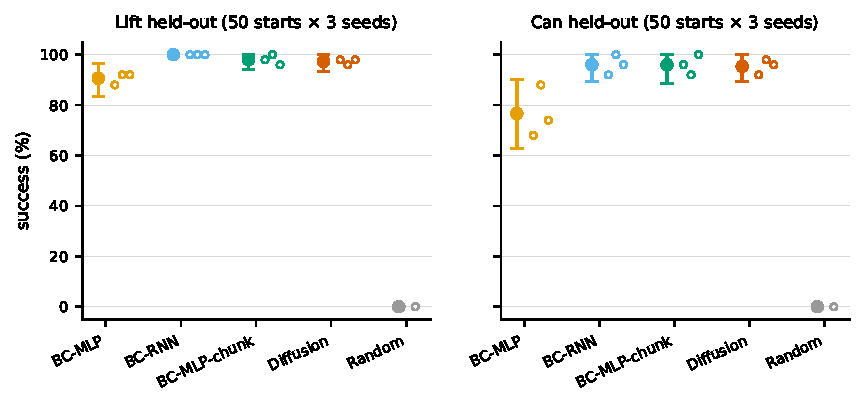
\includegraphics[width=\linewidth]{generated/figures/heldout_success.pdf}
\caption{Held-out success per family and task. Filled markers: mean over seeds with the
bootstrap \rf{proto.level}\,\% interval; open markers: the three training seeds.}
\label{fig:heldout}
\end{figure}

\paragraph{H1.} Every trained family separates from the random-action baseline, which never
succeeds, on both tasks (Table~\ref{tab:differences}).

\paragraph{Lift.} Lift is close to saturated: BC-RNN succeeds on every held-out start
(\rf{l1.lift.bcrnn.succ}\,\%), BC-MLP-chunk on \rf{l1.lift.chunk.succ}\,\% and diffusion on
\rf{l1.lift.diff.succ}\,\%. The only separated learned comparison is H3: BC-RNN exceeds BC-MLP
by \rf{l1.lift.bcrnn-bcmlp.d}\,pp [\rf{l1.lift.bcrnn-bcmlp.lo}, \rf{l1.lift.bcrnn-bcmlp.hi}].
Diffusion's advantage over BC-MLP (\rf{l1.lift.diff-bcmlp.d}\,pp
[\rf{l1.lift.diff-bcmlp.lo}, \rf{l1.lift.diff-bcmlp.hi}]) is not separated, although the
declared secondary outcome, censored episode length, is (\rf{l1.lift.len.diff-bcmlp.d} steps
[\rf{l1.lift.len.diff-bcmlp.lo}, \rf{l1.lift.len.diff-bcmlp.hi}], mostly from success), nor is its
difference from BC-RNN (\rf{l1.lift.diff-bcrnn.d}\,pp) or from BC-MLP-chunk
(\rf{l1.lift.diff-chunk.d}\,pp).

\paragraph{Can.} On Can, BC-MLP is the clear outlier (\rf{l1.can.bcmlp.succ}\,\%), while the
other three families lie within one point of each other (\rf{l1.can.bcrnn.succ},
\rf{l1.can.chunk.succ} and \rf{l1.can.diff.succ}\,\%). The primary H2 comparison is separated:
diffusion exceeds BC-MLP by \rf{l1.can.diff-bcmlp.d}\,pp [\rf{l1.can.diff-bcmlp.lo},
\rf{l1.can.diff-bcmlp.hi}]. The H2-c control does not support attributing that advantage to
the generative model: diffusion minus BC-MLP-chunk is \rf{l1.can.diff-chunk.d}\,pp
[\rf{l1.can.diff-chunk.lo}, \rf{l1.can.diff-chunk.hi}], is not separated (which is not evidence of equality). BC-RNN
also separates from BC-MLP (H3: \rf{l1.can.bcrnn-bcmlp.d}\,pp [\rf{l1.can.bcrnn-bcmlp.lo},
\rf{l1.can.bcrnn-bcmlp.hi}]), although it differs from BC-MLP in its architecture as well as in
its history. With privileged state on these two tasks, these data therefore give no evidence
that the generative head adds to observation history and chunking. That BC-MLP-chunk
(\rf{l1.can.chunk.succ}\,\%) also exceeds BC-MLP (\rf{l1.can.bcmlp.succ}\,\%) is visible in
Table~\ref{tab:heldout}, but it is not a declared comparison and is exploratory. A further difference between the heads, the diffusion sampler's bound on
its actions, is discussed in Section~\ref{sec:limitations}.

\begin{table}[t]
\centering\small
\caption{Declared held-out differences $A - B$ with the hierarchical paired bootstrap's
\rf{proto.level}\,\% interval. Success in percentage points; censored episode length in control steps,
with failures counted at the horizon (negative is faster). Intervals are not adjusted for
the \rf{proto.ncomparisons} success comparisons per task.}
\label{tab:differences}
\resizebox{\linewidth}{!}{% Generated by scripts/paper_assets.py (DECISIONS D-094). Do not edit.
% Sources (path sha256):
%   docs/FINAL_TEST_FREEZE.md 6a3c6874c4bc1857efe46ccb05c0a1fa68247671fc9a96f5f54ce079aa9153e9
%   reports/session7/results/results.json b8b097c38765c588711615917e3cfd5be6847e63083ddebe92f0f1488672408c
\begin{tabular}{llll}
\toprule
 & Difference $A - B$ & Lift & Can \\
\midrule
\multicolumn{4}{l}{\emph{Success (percentage points)}} \\
H1 & BC-MLP $-$ Random (uniform) & \ensuremath{+}90.7 [\ensuremath{+}83.3, \ensuremath{+}96.7], separated (\ensuremath{+}) & \ensuremath{+}76.7 [\ensuremath{+}62.7, \ensuremath{+}90.0], separated (\ensuremath{+}) \\
H1 & BC-RNN $-$ Random (uniform) & \ensuremath{+}100.0 [\ensuremath{+}100.0, \ensuremath{+}100.0], separated (\ensuremath{+}) & \ensuremath{+}96.0 [\ensuremath{+}89.3, \ensuremath{+}100.0], separated (\ensuremath{+}) \\
H1 & BC-MLP-chunk $-$ Random (uniform) & \ensuremath{+}98.0 [\ensuremath{+}94.0, \ensuremath{+}100.0], separated (\ensuremath{+}) & \ensuremath{+}96.0 [\ensuremath{+}88.7, \ensuremath{+}100.0], separated (\ensuremath{+}) \\
H1 & Diffusion U-Net $-$ Random (uniform) & \ensuremath{+}97.3 [\ensuremath{+}93.3, \ensuremath{+}100.0], separated (\ensuremath{+}) & \ensuremath{+}95.3 [\ensuremath{+}89.3, \ensuremath{+}100.0], separated (\ensuremath{+}) \\
H2 & Diffusion U-Net $-$ BC-MLP & \ensuremath{+}6.7 [\ensuremath{-}0.7, \ensuremath{+}14.7], not separated & \ensuremath{+}18.7 [\ensuremath{+}4.7, \ensuremath{+}32.7], separated (\ensuremath{+}) \\
H2 & Diffusion U-Net $-$ BC-RNN & \ensuremath{-}2.7 [\ensuremath{-}6.7, \ensuremath{+}0.0], not separated & \ensuremath{-}0.7 [\ensuremath{-}8.0, \ensuremath{+}6.7], not separated \\
H2-c & Diffusion U-Net $-$ BC-MLP-chunk & \ensuremath{-}0.7 [\ensuremath{-}5.3, \ensuremath{+}4.7], not separated & \ensuremath{-}0.7 [\ensuremath{-}8.7, \ensuremath{+}7.3], not separated \\
H3 & BC-RNN $-$ BC-MLP & \ensuremath{+}9.3 [\ensuremath{+}3.3, \ensuremath{+}16.7], separated (\ensuremath{+}) & \ensuremath{+}19.3 [\ensuremath{+}5.3, \ensuremath{+}34.0], separated (\ensuremath{+}) \\
\midrule
\multicolumn{4}{l}{\emph{Censored episode length (steps; failures count 400)}} \\
H2 & Diffusion U-Net $-$ BC-MLP & \ensuremath{-}28.9 [\ensuremath{-}59.4, \ensuremath{-}1.6], separated (\ensuremath{-}) & \ensuremath{-}56.0 [\ensuremath{-}98.0, \ensuremath{-}14.7], separated (\ensuremath{-}) \\
H2 & Diffusion U-Net $-$ BC-RNN & \ensuremath{+}11.0 [\ensuremath{+}1.1, \ensuremath{+}25.1], separated (\ensuremath{+}) & \ensuremath{+}2.1 [\ensuremath{-}18.5, \ensuremath{+}22.7], not separated \\
H2-c & Diffusion U-Net $-$ BC-MLP-chunk & \ensuremath{+}2.8 [\ensuremath{-}15.6, \ensuremath{+}20.0], not separated & \ensuremath{+}9.5 [\ensuremath{-}13.0, \ensuremath{+}33.3], not separated \\
H3 & BC-RNN $-$ BC-MLP & \ensuremath{-}39.9 [\ensuremath{-}67.8, \ensuremath{-}16.2], separated (\ensuremath{-}) & \ensuremath{-}58.1 [\ensuremath{-}100.3, \ensuremath{-}16.7], separated (\ensuremath{-}) \\
\bottomrule
\end{tabular}
}
\end{table}

\begin{figure}[t]
\centering
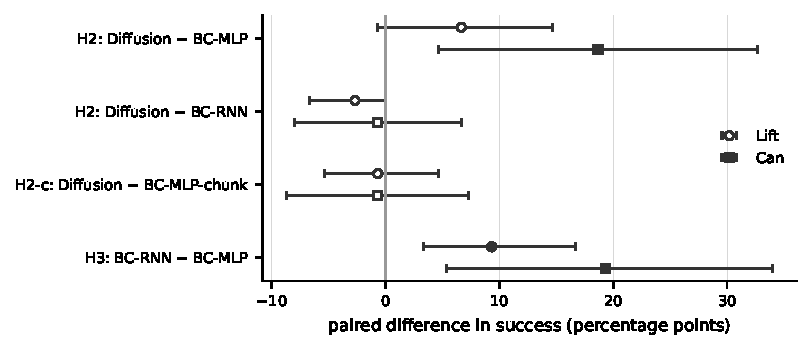
\includegraphics[width=\linewidth]{generated/figures/differences.pdf}
\caption{The H2, H2-c and H3 differences in held-out success with their \rf{proto.level}\,\% intervals.
Filled markers are separated (the interval excludes zero).}
\label{fig:differences}
\end{figure}

\paragraph{How much the verdicts depend on the interval method.} The seed-level sensitivity
analysis (Section~\ref{sec:protocol}; Table~\ref{tab:sens-main}; not preregistered) changes
\rf{sens.l1.changed} of the \rf{sens.l1.n} Level~1 verdicts. Both separated Can comparisons
among learned families lose separation: diffusion minus BC-MLP becomes
[\rf{sens.l1.can.diff-bcmlp.lo}, \rf{sens.l1.can.diff-bcmlp.hi}] with
\rf{sens.l1.can.diff-bcmlp.df} degrees of freedom, and BC-RNN minus BC-MLP
[\rf{sens.l1.can.bcrnn-bcmlp.lo}, \rf{sens.l1.can.bcrnn-bcmlp.hi}], because BC-MLP's three
Can seeds differ widely (Table~\ref{tab:heldout}). Lift's diffusion minus BC-MLP, not
separated by the bootstrap, becomes separated ([\rf{sens.l1.lift.diff-bcmlp.lo},
\rf{sens.l1.lift.diff-bcmlp.hi}]). The frozen verdicts stand as the preregistered result, but
the Can H2 and H3 separations rest on three BC-MLP seeds and should be read as fragile. No
H2-c verdict changes under either method.

\paragraph{Censored episode length.} Length differences are dominated by failures, which
count \rf{proto.horizon} steps. We split each difference exactly into a success part,
$-(p_A - p_B)(H - \bar T_B)$, and a speed part, $p_A(\bar T_A - \bar T_B)$, where $p$ is the
success rate, $\bar T$ the mean first-success step of successes and $H$ the horizon (D-095;
not preregistered). Diffusion's separated length advantage over BC-MLP on Can
(\rf{l1.can.len.diff-bcmlp.d} steps) is almost all success (\rf{l1.can.len.diff-bcmlp.succpart}
from success, \rf{l1.can.len.diff-bcmlp.speedpart} from speed). Its separated length
\emph{disadvantage} against BC-RNN on Lift (\rf{l1.lift.len.diff-bcrnn.d} steps) is also
mostly success (\rf{l1.lift.len.diff-bcrnn.succpart} from diffusion's few failures, against
\rf{l1.lift.len.diff-bcrnn.speedpart} from speed). Censored length therefore restates the
success comparison and adds little independent evidence about speed.

\paragraph{Selected checkpoints.} The selected training steps are listed per run in
Table~\ref{tab:checkpoints}. Of the \rf{l1.bc.nruns} BC runs, \rf{l1.bc.first-ckpt} selected
their first checkpoint, so for them the budget was more than enough and earlier checkpoints
were not examined; two diffusion runs (the first Lift seed and the second Can seed) selected their final
checkpoint (\rf{l1.lift.diff.step.s0} and \rf{l1.can.diff.step.s1} steps), so a longer budget
might have helped them.

\paragraph{Secondary metrics.} Table~\ref{tab:secondary} reports the protocol's declared
secondary metrics, which every held-out summary computed per episode but no frozen analysis
aggregated (audit C-9; D-096). They are descriptive only, without intervals. The mean absolute
step-to-step change of the executed motion command is \rf{sec.lift.diff.delta} for diffusion
and \rf{sec.lift.chunk.delta} for BC-MLP-chunk on Lift; BC-MLP has the largest clip fraction
(\rf{sec.lift.bcmlp.clip}\,\% on Lift), and diffusion's is zero by construction of its sampler
(Section~\ref{sec:limitations}).

\begin{table}[t]
\centering\small
\caption{Declared secondary metrics on the held-out starts, aggregated after the frozen
analysis (D-096; plain means, no intervals). Gripper sign changes per episode, with the range
of the per-seed means; mean absolute step-to-step change of the executed motion command; and
the clip fraction, the frozen mean over the six motion dimensions of the share of actions
clipped to the controller limits. All depend on episode length, which ends at first success.}
\label{tab:secondary}
\resizebox{\linewidth}{!}{% Generated by scripts/paper_assets.py (DECISIONS D-094). Do not edit.
% Sources (path sha256):
%   reports/session7/results/results.json b8b097c38765c588711615917e3cfd5be6847e63083ddebe92f0f1488672408c
% Plus 26 files hash-chained from the sources above, listed in index.json.
\begin{tabular}{llrrrr}
\toprule
Task & Family & Episodes & Gripper sign changes & Mean $|\Delta a|$ (motion) & Clipped motion actions (\%) \\
\midrule
Lift & BC-MLP & 150 & 3.06 [1.46, 5.56] & 0.017 & 15.7 \\
Lift & BC-RNN & 150 & 1.03 [1.00, 1.08] & 0.019 & 0.0 \\
Lift & BC-MLP-chunk & 150 & 2.30 [1.00, 3.60] & 0.026 & 4.5 \\
Lift & Diffusion U-Net & 150 & 2.31 [1.90, 3.02] & 0.036 & 0.0 \\
Lift & Random (uniform) & 50 & 197.78 & 0.670 & 0.0 \\
\addlinespace
Can & BC-MLP & 150 & 6.04 [3.24, 9.02] & 0.020 & 9.5 \\
Can & BC-RNN & 150 & 1.97 [1.96, 2.00] & 0.022 & 2.4 \\
Can & BC-MLP-chunk & 150 & 2.73 [2.00, 3.96] & 0.025 & 3.8 \\
Can & Diffusion U-Net & 150 & 2.57 [2.42, 2.70] & 0.043 & 0.0 \\
Can & Random (uniform) & 50 & 198.76 & 0.666 & 0.0 \\
\bottomrule
\end{tabular}
}
\end{table}

\paragraph{Cost and latency.} Table~\ref{tab:cost} lists training cost and inference latency.
On the CPU, a diffusion run costs \rf{l1.ratio.cpu.lo}--\rf{l1.ratio.cpu.hi} times the CPU
hours of a BC-MLP-chunk run, and a diffusion decision (\rf{diff.ddim} DDIM steps) takes
\rf{l1.ratio.lat.lo}--\rf{l1.ratio.lat.hi} times as long, for no measured gain in held-out
success over that control (it did gain under the Lift arm offset;
Section~\ref{sec:robustness}). Every Level~1 run trained locally at no billed cost. The table's latencies come
from two methods (a dedicated benchmark for Level~1, medians recorded during the held-out
rollouts for the GPU-trained studies) and are comparable only within a block. The step time of the first
Level~2 training seed printed by the frozen analysis was wrong; the table shows the frozen value
beside the corrected one (KI-049). Table~\ref{tab:spend} reconciles all paid compute: \rf{spend.launches}
launches, \$\rf{spend.total} in total, each under a committed approval and within its dollar
cap; one approval's launch count was exceeded before it was amended
(Section~\ref{sec:limitations}).

\begin{table}[t]
\centering\small
\caption{Training cost and inference latency. Level~1 CPU hours are per training seed;
latency is the median time of one decision (observation to action or action chunk); chunked policies decide every \rf{hor.exec} control steps. Billed amounts are Modal's usage report at list price
before credits.}
\label{tab:cost}
\resizebox{\linewidth}{!}{% Generated by scripts/paper_assets.py (DECISIONS D-094). Do not edit.
% Sources (path sha256):
%   reports/session7/results/results.json b8b097c38765c588711615917e3cfd5be6847e63083ddebe92f0f1488672408c
%   reports/session9/level2_results/ERRATA.md 280974a994408a6f7d3683788561f0f6c05de90f4eccf8d7b1636dd90fabca31
%   reports/session9/level2_results/results.json 1d33c975e49df907a6543b17e0cf36d047f7b5ce11aa69a355313e146c22571e
%   logs/session9/pc_train/launch_records/train_gpu_pc_20261109T130430.result.json 0ea097359ba49b375e3ce53199435b771e9c3253e1e039baa62f71a003e2a737
%   reports/session8/rgb_results/results.json 57663b81aafc70e9c1d850322b6bb1b894f7dad0d082976b1f546475a601390e
\begin{tabular}{llrrr}
\toprule
Run & Hardware and training time & Latency ms & ms/step & Billed \\
\midrule
\multicolumn{5}{l}{\emph{Level 1: training on local CPU (one torch thread); latency: dedicated benchmark, canonical container}} \\
Lift BC-MLP & CPU 0.22, 0.17, 0.17 CPU-h & 0.91 & -- & \$0.00 \\
Lift BC-RNN & CPU 1.20, 0.93, 0.93 CPU-h & 9.04 & -- & \$0.00 \\
Lift BC-MLP-chunk & CPU 0.17, 0.18, 0.18 CPU-h & 1.66 & -- & \$0.00 \\
Lift Diffusion U-Net & CPU 4.42, 3.36, 3.36 CPU-h & 36.95 & -- & \$0.00 \\
Can BC-MLP & CPU 0.22, 0.16, 0.16 CPU-h & 1.08 & -- & \$0.00 \\
Can BC-RNN & CPU 1.27, 0.85, 0.85 CPU-h & 9.00 & -- & \$0.00 \\
Can BC-MLP-chunk & CPU 0.18, 0.18, 0.18 CPU-h & 1.42 & -- & \$0.00 \\
Can Diffusion U-Net & CPU 4.31, 3.99, 3.98 CPU-h & 37.71 & -- & \$0.00 \\
\midrule
\multicolumn{5}{l}{\emph{RGB study (Lift): training on one NVIDIA L4; latency: median of episode medians during the held-out run}} \\
Visual BC-chunk seed 0 & L4 1.01 h, 2 segments & 66.4 & -- & \$1.14 \\
Visual BC-chunk seed 1 & L4 1.01 h, 2 segments & 65.0 & -- & \$1.14 \\
Visual BC-chunk seed 2 & L4 1.00 h, 2 segments & 63.0 & -- & \$1.13 \\
Visual diffusion seed 0 & L4 1.35 h, 2 segments & 183.1 & -- & \$1.52 \\
Visual diffusion seed 1 & L4 1.36 h, 2 segments & 187.2 & -- & \$1.53 \\
Visual diffusion seed 2 & L4 1.29\textsuperscript{b} h, 3 segments & 166.4 & -- & \$1.60 \\
\midrule
\multicolumn{5}{l}{\emph{Level 2 (Lift): training on one NVIDIA L4; latency: median of episode medians during the held-out run}} \\
Point-cloud diffusion seed 0 & L4 0.41\textsuperscript{a} h, 3 segments & 147.4 & 24.62 $\to$ \textbf{42.2}\textsuperscript{a} & \$0.80 \\
Point-cloud diffusion seed 1 & L4 0.70 h, 1 segment & 146.0 & 41.73 & \$0.78 \\
Point-cloud diffusion seed 2 & L4 0.71 h, 1 segment & 147.0 & 42.55 & \$0.80 \\
\midrule
\multicolumn{5}{p{0.95\linewidth}}{\footnotesize\textsuperscript{a} Erratum (KI-049, \texttt{ERRATA.md}, SHA-256 \texttt{280974a9}): the frozen analysis printed the left value. The corrected step time is the completing launch's training time over the steps it trained, from its committed launch record; the hours are that segment only and leave out the cut first segment (\texttt{ERRATA.md} gives the total).} \\
\multicolumn{5}{p{0.95\linewidth}}{\footnotesize\textsuperscript{b} One launch of this run was preempted and restarted; the preempted attempt recorded no training time, so the hours leave it out, while the billed amount includes it (KI-044; audit C-6).} \\
\bottomrule
\end{tabular}
}
\end{table}

\begin{table}[t]
\centering\small
\caption{Paid compute by approval, reconciled with the cost ledger's billing events.}
\label{tab:spend}
% Generated by scripts/paper_assets.py (DECISIONS D-094). Do not edit.
% Sources (path sha256):
%   reports/compute/cost_ledger.jsonl a4f92b9f1f4ae3708bacea7a34946b3a51705205b1fc4e4a2666096f3ba40578
\begin{tabular}{lllrrr}
\toprule
Approval & Gate & Functions & Billed launches & Cap & Billed \\
\midrule
A-01 & Gate A & \texttt{gpu\_probe}, \texttt{train\_cpu} & 6 & \$2.00 & \$0.1483 \\
A-02 & Gate D (RGB probe) & \texttt{rgb\_probe} & 1 & \$1.00 & \$0.0317 \\
A-03 & Gate D2 (RGB main) & \texttt{train\_gpu} & 12 & \$15.00 & \$8.0598 \\
A-04 & Level 2 (point cloud) & \texttt{train\_gpu\_pc} & 5 & \$9.00 & \$2.3747 \\
\midrule
Total &  &  & 24 &  & \$10.6144 \\
\bottomrule
\end{tabular}

\end{table}

\begin{figure}[t]
\centering
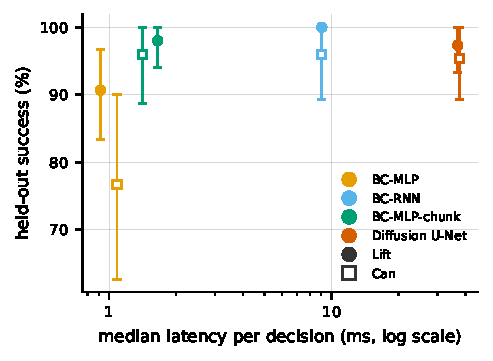
\includegraphics[width=0.8\linewidth]{generated/figures/latency_success.pdf}
\caption{Held-out success against the median latency of one decision (log scale) for the
Level~1 families, with the bootstrap interval. Filled circles: Lift; open squares: Can.}
\label{fig:latency}
\end{figure}

\section{Robustness and ablations (Level 1)}
\label{sec:robustness}

\paragraph{Design.} H4 tests two perturbations defined, validated and committed before the
first robustness rollout. \emph{Cube shift} (Lift only) moves the cube's centre to a radius
drawn uniformly between \rf{rob.cube.rmin} and \rf{rob.cube.rmax}\,cm from the table centre,
at a uniform angle; the demonstrations place it within $\pm$\rf{rob.cube.train}\,cm in each
direction, so every shifted cube lies outside the training square. \emph{Arm offset} (Lift
and Can) adds $\pm$\rf{rob.arm.rad}\,rad with independent random signs to every arm joint,
\rf{rob.arm.ratio} times the standard deviation (\rf{rob.arm.sigma}\,rad) of robosuite's own
joint noise. Can has no placement set because its can is already sampled over the whole source
bin. Each perturbed state is derived from the base state with the same index and passes
validity checks (exact restore, no success at the start, joint limits, no new contacts or
penetration, and passive settling). The \rf{proto.nseeds} selected checkpoints of each family
run every base and perturbed start once. Since the base starts selected nothing, these results
are not biased by selection, but they were run before the held-out test and are not part of
it. Differences are paired by base index, and the bootstrap is the one of
Section~\ref{sec:protocol}.

\begin{table}[t]
\centering\small
\caption{Success (\%) on the robustness base starts and the two perturbation sets, mean over
seeds with the bootstrap \rf{proto.level}\,\% interval.}
\label{tab:robustness}
\resizebox{\linewidth}{!}{% Generated by scripts/paper_assets.py (DECISIONS D-094). Do not edit.
% Sources (path sha256):
%   reports/session7/robustness/analysis.json 8cca66a8a8a8cecf0b734355167936e81983c821c625a23456523365409c9451
\begin{tabular}{lrrrrr}
\toprule
Family & Lift base & Lift cube shift & Lift arm offset & Can base & Can arm offset \\
\midrule
BC-MLP & 98.0 [92.0, 100.0] & 52.7 [35.3, 69.3] & 22.7 [12.0, 34.0] & 69.3 [56.0, 82.0] & 30.0 [19.3, 41.3] \\
BC-RNN & 100.0 [100.0, 100.0] & 96.0 [88.0, 100.0] & 50.0 [36.0, 64.0] & 96.7 [91.3, 100.0] & 53.3 [41.3, 66.0] \\
BC-MLP-chunk & 100.0 [100.0, 100.0] & 54.7 [33.3, 75.3] & 48.7 [36.0, 61.3] & 95.3 [89.3, 100.0] & 79.3 [66.0, 90.7] \\
Diffusion U-Net & 99.3 [96.0, 100.0] & 85.3 [76.0, 93.3] & 88.0 [79.3, 95.3] & 92.0 [85.3, 98.0] & 71.3 [58.0, 84.0] \\
\bottomrule
\end{tabular}
}
\end{table}

\begin{figure}[t]
\centering
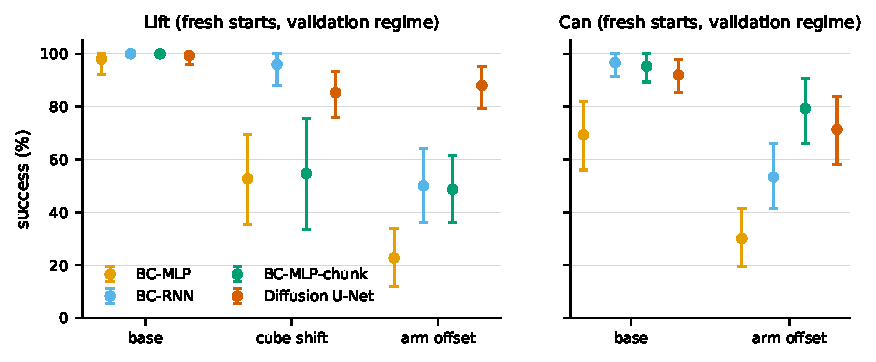
\includegraphics[width=\linewidth]{generated/figures/robustness.pdf}
\caption{Success per family on the base starts and under each perturbation (mean over seeds
with the \rf{proto.level}\,\% interval).}
\label{fig:robustness}
\end{figure}

\paragraph{Lift.} All four families succeed on at least \rf{rob.lift.bcmlp.base.succ}\,\% of
the base starts (Table~\ref{tab:robustness}, Figure~\ref{fig:robustness}). Under cube shift,
BC-MLP and BC-MLP-chunk fall to \rf{rob.lift.bcmlp.cube.succ} and
\rf{rob.lift.chunk.cube.succ}\,\%, diffusion to \rf{rob.lift.diff.cube.succ}\,\%, and BC-RNN
holds at \rf{rob.lift.bcrnn.cube.succ}\,\%. Under arm offset, diffusion keeps
\rf{rob.lift.diff.arm.succ}\,\%, against \rf{rob.lift.bcrnn.arm.succ}\,\% for BC-RNN,
\rf{rob.lift.chunk.arm.succ}\,\% for BC-MLP-chunk and \rf{rob.lift.bcmlp.arm.succ}\,\% for
BC-MLP. Diffusion exceeds BC-MLP-chunk on both sets (\rf{rob.lift.cube.diff-chunk.d} and
\rf{rob.lift.arm.diff-chunk.d}\,pp, both separated) and BC-RNN under arm offset
(\rf{rob.lift.arm.diff-bcrnn.d}\,pp, separated), while BC-RNN is ahead under cube shift
(diffusion minus BC-RNN \rf{rob.lift.cube.diff-bcrnn.d}\,pp, not separated).

\paragraph{Can.} The Lift pattern does not carry over. Under arm offset on Can, BC-MLP-chunk
keeps \rf{rob.can.chunk.arm.succ}\,\% and diffusion \rf{rob.can.diff.arm.succ}\,\%; their
difference (\rf{rob.can.arm.diff-chunk.d}\,pp [\rf{rob.can.arm.diff-chunk.lo},
\rf{rob.can.arm.diff-chunk.hi}]) is not separated. Diffusion does exceed BC-MLP
(\rf{rob.can.arm.diff-bcmlp.d}\,pp) and BC-RNN (\rf{rob.can.arm.diff-bcrnn.d}\,pp).

\paragraph{Reading H4.} Each Lift and Can analysis reports \rf{rob.lift.contrasts} and
\rf{rob.can.contrasts} differences and contrasts, unadjusted for multiplicity. The seed-level
sensitivity analysis (Table~\ref{tab:sens-rob} in the appendix) changes
\rf{sens.rob.changed} of \rf{sens.rob.n} robustness verdicts, all from separated to not
separated. Among them is diffusion's advantage over BC-MLP-chunk under Lift cube shift
([\rf{sens.rob.lift.cube.diff-chunk.lo}, \rf{sens.rob.lift.cube.diff-chunk.hi}]), whereas its
advantage under Lift arm offset stays separated under both methods. Two further
cautions apply. First, the diffusion sampler bounds every action to the range of the
training actions, while the BC heads are bounded only by the controller limits. In BC
episodes that fail under perturbation most motion actions lie outside that range, which
diffusion cannot do, so the between-family robustness gaps combine the generative model with
this output bound (Section~\ref{sec:limitations}). This is a correlation, not a mechanism:
the out-of-range actions start only after a grasp is missed, and BC-RNN rarely leaves the
range yet keeps only \rf{rob.lift.bcrnn.arm.succ}\,\% under arm offset. Second, the results hold
only for these two perturbations. We therefore read H4 as: on Lift, diffusion degrades least
under a large joint offset, and under cube shift BC-RNN degrades least, with diffusion not
separated from it; on Can, diffusion's drop under arm offset is not separated from the
chunked MLP's (\rf{rob.can.dd.arm.diff-chunk.d}\,pp [\rf{rob.can.dd.arm.diff-chunk.lo},
\rf{rob.can.dd.arm.diff-chunk.hi}]), whose point estimate is smaller.

\paragraph{Ablations.} Table~\ref{tab:ablations} reports the three preregistered diffusion
ablations on the robustness base starts. A1 evaluates the raw trained weights instead of
the EMA weights of the same checkpoints; A2 samples with DDPM over all \rf{diff.T} steps
instead of DDIM with \rf{diff.ddim}; A3 (Can only) trains a diffusion policy with one
observation instead of two (\rf{abl.A3.params.to1} instead of \rf{abl.A3.params.to2}
parameters, three new seeds, selected by the same rule). Checkpoints were selected with EMA
weights and DDIM-\rf{diff.ddim}, which favours the primary arm in A1 and A2, and all three
ablations share the primary arm's evaluations on the base starts, so they are not
independent of each other or of H4. None of the five differences is separated, by the
bootstrap or by the seed-level analysis. DDIM-\rf{diff.ddim} was not separated from DDPM over
all \rf{diff.T} steps, although both point estimates favour DDPM (\rf{abl.lift.A2.d} and
\rf{abl.can.A2.d}\,pp). No ablation of the action horizons ($T_p$, $T_a$) was run; the only comparison
that changes them is BC-MLP against BC-MLP-chunk, which also changes the observation window
and is not a declared comparison.

\begin{table}[t]
\centering\small
\caption{Diffusion ablations on the robustness base starts (\rf{proto.nseeds} seeds,
\rf{proto.nstates} starts each). A1 and A2 re-evaluate the selected checkpoints; A3 trains
separately. Primary: EMA weights, DDIM-10, $T_o = 2$.}
\label{tab:ablations}
\resizebox{\linewidth}{!}{% Generated by scripts/paper_assets.py (DECISIONS D-094). Do not edit.
% Sources (path sha256):
%   reports/session7/robustness/analysis.json 8cca66a8a8a8cecf0b734355167936e81983c821c625a23456523365409c9451
\begin{tabular}{llllll}
\toprule
 & Task & Arm $A$ (success \%) & Arm $B$ (success \%) & $A - B$ (pp) & Outcome \\
\midrule
A1 & Lift & primary 99.3 [96.0, 100.0] & trained weights 98.7 [95.3, 100.0] & \ensuremath{+}0.7 [\ensuremath{+}0.0, \ensuremath{+}2.7] & not separated \\
A1 & Can & primary 92.0 [84.7, 98.0] & trained weights 94.7 [88.7, 99.3] & \ensuremath{-}2.7 [\ensuremath{-}7.3, \ensuremath{+}0.7] & not separated \\
A2 & Lift & primary 99.3 [96.0, 100.0] & DDPM-100 100.0 [100.0, 100.0] & \ensuremath{-}0.7 [\ensuremath{-}4.0, \ensuremath{+}0.0] & not separated \\
A2 & Can & primary 92.0 [84.7, 98.0] & DDPM-100 95.3 [89.3, 100.0] & \ensuremath{-}3.3 [\ensuremath{-}10.0, \ensuremath{+}3.3] & not separated \\
A3 & Can & $T_o = 2$ 92.0 [84.7, 98.0] & $T_o = 1$ 94.0 [86.7, 99.3] & \ensuremath{-}2.0 [\ensuremath{-}8.7, \ensuremath{+}4.0] & not separated \\
\bottomrule
\end{tabular}
}
\end{table}

\paragraph{Failure modes.} Table~\ref{tab:taxonomy} and Figure~\ref{fig:taxonomy} classify
every held-out and Level~2 failure, and Table~\ref{tab:taxonomy-rob} every failure of the
robustness evaluations. Under Lift arm offset, BC-MLP's failures are mostly drifts
(\rf{rob.lift.bcmlp.arm.tax.no-grasp-drift} of its episodes), while diffusion has
\rf{rob.lift.diff.arm.tax.no-grasp-drift} drifts and fails mostly next to the cube
(\rf{rob.lift.diff.arm.tax.no-grasp-near}). On the Level~1 held-out starts, BC-MLP's Lift failures are mostly drifts away
from the cube without a grasp (\rf{l1.lift.bcmlp.tax.no-grasp-drift} of
\rf{l1.lift.n}$\times$\rf{proto.nseeds} episodes), while diffusion's few failures end near the
cube or after a drop. On Can, BC-MLP fails in several ways, most often by never closing the
gripper (\rf{l1.can.bcmlp.tax.gripper-never-closed} episodes). The point-cloud policy's
failures under cube shift are mostly misses near the cube (\rf{l2.pcdiff.cube.tax.no-grasp-near})
and drops (\rf{l2.pcdiff.cube.tax.dropped}), not drifts.

\begin{table}[t]
\centering\small
\caption{Failure taxonomy: episodes per category, summed over the three seeds (one run of
\rf{proto.nstates} episodes for the random baseline).}
\label{tab:taxonomy}
% Generated by scripts/paper_assets.py (DECISIONS D-094). Do not edit.
% Sources (path sha256):
%   reports/session7/results/results.json b8b097c38765c588711615917e3cfd5be6847e63083ddebe92f0f1488672408c
%   reports/session9/level2_results/results.json 1d33c975e49df907a6543b17e0cf36d047f7b5ce11aa69a355313e146c22571e
%   reports/session8/rgb_results/results.json 57663b81aafc70e9c1d850322b6bb1b894f7dad0d082976b1f546475a601390e
\begin{tabular}{lrrrrrrrr}
\toprule
Policy & \rotatebox{90}{success} & \rotatebox{90}{engineering error} & \rotatebox{90}{gripper never closed} & \rotatebox{90}{no grasp, drifted} & \rotatebox{90}{no grasp, near} & \rotatebox{90}{timeout holding} & \rotatebox{90}{in goal bin, not success} & \rotatebox{90}{dropped} \\
\midrule
\multicolumn{9}{l}{\emph{Level 1 held-out, Lift}} \\
BC-MLP & 136 & 0 & 0 & 12 & 0 & 0 & 0 & 2 \\
BC-RNN & 150 & 0 & 0 & 0 & 0 & 0 & 0 & 0 \\
BC-MLP-chunk & 147 & 0 & 0 & 3 & 0 & 0 & 0 & 0 \\
Diffusion U-Net & 146 & 0 & 0 & 0 & 3 & 0 & 0 & 1 \\
Random (uniform) & 0 & 0 & 0 & 38 & 9 & 0 & 0 & 3 \\
\multicolumn{9}{l}{\emph{Level 1 held-out, Can}} \\
BC-MLP & 115 & 0 & 11 & 8 & 4 & 3 & 2 & 7 \\
BC-RNN & 144 & 0 & 1 & 1 & 0 & 0 & 3 & 1 \\
BC-MLP-chunk & 144 & 0 & 1 & 0 & 4 & 0 & 1 & 0 \\
Diffusion U-Net & 143 & 0 & 0 & 2 & 0 & 0 & 3 & 2 \\
Random (uniform) & 0 & 0 & 0 & 44 & 6 & 0 & 0 & 0 \\
\multicolumn{9}{l}{\emph{RGB study held-out, Lift}} \\
Visual diffusion & 150 & 0 & 0 & 0 & 0 & 0 & 0 & 0 \\
Visual BC-chunk & 149 & 0 & 0 & 0 & 1 & 0 & 0 & 0 \\
\multicolumn{9}{l}{\emph{Level 2, Lift}} \\
Point-cloud diffusion, held-out & 150 & 0 & 0 & 0 & 0 & 0 & 0 & 0 \\
Point-cloud diffusion, cube shift & 85 & 0 & 0 & 4 & 45 & 0 & 0 & 16 \\
Point-cloud diffusion, base & 150 & 0 & 0 & 0 & 0 & 0 & 0 & 0 \\
Visual diffusion, cube shift & 147 & 0 & 0 & 0 & 3 & 0 & 0 & 0 \\
Visual diffusion, base & 150 & 0 & 0 & 0 & 0 & 0 & 0 & 0 \\
\bottomrule
\end{tabular}

\end{table}

\begin{table}[t]
\centering\small
\caption{Failure taxonomy of the robustness evaluations (validation regime), summed over the
three seeds.}
\label{tab:taxonomy-rob}
% Generated by scripts/paper_assets.py (DECISIONS D-094). Do not edit.
% Sources (path sha256):
%   reports/session7/robustness/analysis.json 8cca66a8a8a8cecf0b734355167936e81983c821c625a23456523365409c9451
\begin{tabular}{lrrrrrrrr}
\toprule
Policy & \rotatebox{90}{success} & \rotatebox{90}{engineering error} & \rotatebox{90}{gripper never closed} & \rotatebox{90}{no grasp, drifted} & \rotatebox{90}{no grasp, near} & \rotatebox{90}{timeout holding} & \rotatebox{90}{in goal bin, not success} & \rotatebox{90}{dropped} \\
\midrule
\multicolumn{9}{l}{\emph{Lift, base}} \\
BC-MLP & 147 & 0 & 0 & 3 & 0 & 0 & 0 & 0 \\
BC-RNN & 150 & 0 & 0 & 0 & 0 & 0 & 0 & 0 \\
BC-MLP-chunk & 150 & 0 & 0 & 0 & 0 & 0 & 0 & 0 \\
Diffusion U-Net & 149 & 0 & 0 & 0 & 0 & 0 & 0 & 1 \\
\multicolumn{9}{l}{\emph{Lift, cube shift}} \\
BC-MLP & 79 & 0 & 5 & 57 & 1 & 0 & 0 & 8 \\
BC-RNN & 144 & 0 & 0 & 4 & 0 & 0 & 0 & 2 \\
BC-MLP-chunk & 82 & 0 & 0 & 49 & 7 & 0 & 0 & 12 \\
Diffusion U-Net & 128 & 0 & 0 & 1 & 15 & 0 & 0 & 6 \\
\multicolumn{9}{l}{\emph{Lift, arm offset}} \\
BC-MLP & 34 & 0 & 2 & 104 & 6 & 0 & 0 & 4 \\
BC-RNN & 75 & 0 & 7 & 57 & 5 & 0 & 0 & 6 \\
BC-MLP-chunk & 73 & 0 & 0 & 67 & 3 & 0 & 0 & 7 \\
Diffusion U-Net & 132 & 0 & 0 & 0 & 12 & 1 & 0 & 5 \\
\multicolumn{9}{l}{\emph{Can, base}} \\
BC-MLP & 104 & 0 & 16 & 9 & 4 & 2 & 8 & 7 \\
BC-RNN & 145 & 0 & 1 & 1 & 0 & 0 & 2 & 1 \\
BC-MLP-chunk & 143 & 0 & 2 & 1 & 1 & 0 & 1 & 2 \\
Diffusion U-Net & 138 & 0 & 0 & 0 & 2 & 1 & 4 & 5 \\
\multicolumn{9}{l}{\emph{Can, arm offset}} \\
BC-MLP & 45 & 0 & 17 & 60 & 13 & 0 & 6 & 9 \\
BC-RNN & 80 & 0 & 6 & 43 & 2 & 6 & 4 & 9 \\
BC-MLP-chunk & 119 & 0 & 5 & 8 & 9 & 0 & 3 & 6 \\
Diffusion U-Net & 107 & 0 & 8 & 7 & 8 & 0 & 4 & 16 \\
\bottomrule
\end{tabular}

\end{table}

\begin{figure}[t]
\centering
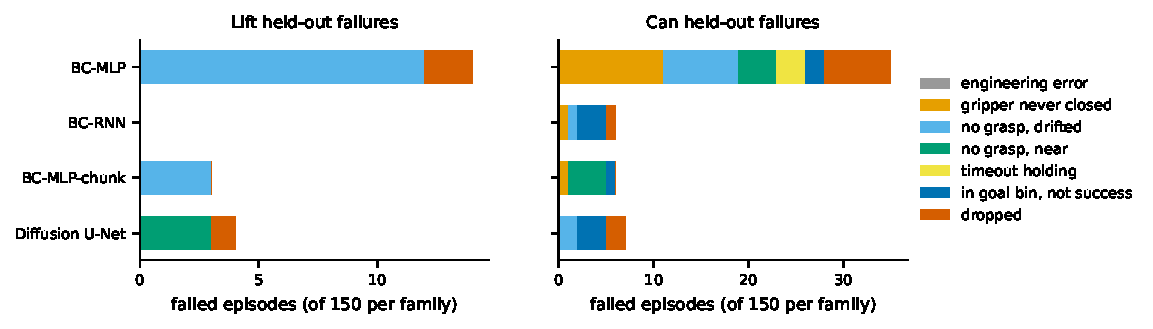
\includegraphics[width=\linewidth]{generated/figures/taxonomy.pdf}
\caption{Failure categories of the Level~1 held-out episodes per family (successes omitted).}
\label{fig:taxonomy}
\end{figure}

\section{Observation-modality extensions (Lift)}
\label{sec:perception}

Both extensions replace the privileged object pose by sensor observations, each under its
own freeze committed before its first training launch. They share Lift's demonstrations,
split, proprioception, action encoding, diffusion head and horizons. Neither is compared
causally with Level~1: the Level~1 families trained longer on a CPU, received
\rf{train.trials} tuning trials each (the extensions received none), and saw the exact object
pose, so a Level~1 number placed beside an extension's number on the same starts is context,
not a comparison. Figure~\ref{fig:renders} shows the scenes and the point cloud.

\begin{figure}[t]
\centering
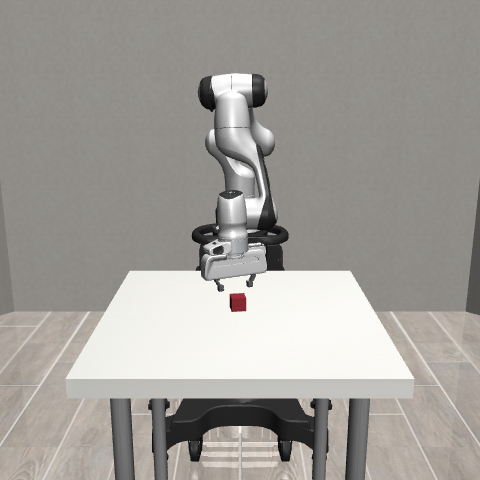
\includegraphics[width=0.32\linewidth]{generated/figures/render_lift.png}\hfill
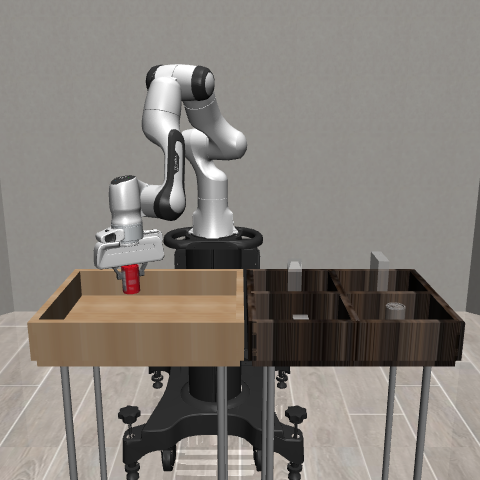
\includegraphics[width=0.32\linewidth]{generated/figures/render_can.png}\hfill
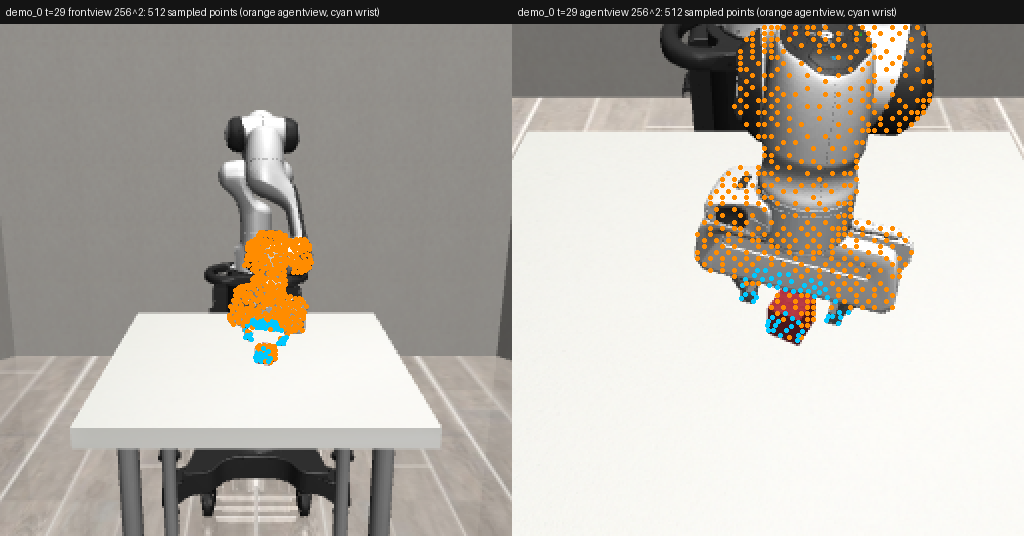
\includegraphics[width=0.32\linewidth]{generated/figures/render_pc_overlay.png}
\caption{Illustrations, not selected for outcome. Left and centre: MuJoCo renders of recorded
held-out states of the Lift and Can diffusion policies (first training seed, first held-out
start; both episodes succeeded), regenerated from the stored simulator state. Right:
the \rf{pc.points} sampled points of one Lift demonstration frame, projected onto the
camera images.}
\label{fig:renders}
\end{figure}

\subsection{RGB study: visual BC versus visual diffusion}
Table~\ref{tab:rgb} gives the result. Both arms are saturated on the Lift held-out starts:
visual diffusion succeeds on \rf{rgb.rgbdiff.k} of \rf{rgb.rgbdiff.n} episodes and visual
BC-chunk on \rf{rgb.rgbbc.k}. The preregistered difference, \rf{rgb.diff-bc.d}\,pp
[\rf{rgb.diff-bc.lo}, \rf{rgb.diff-bc.hi}], is not separated, and the seed-level interval
agrees ([\rf{sens.rgb.diff-bc.lo}, \rf{sens.rgb.diff-bc.hi}]). With both arms at or near
\rf{proto.nstates} of \rf{proto.nstates} per seed, this test cannot distinguish them; a
harder task or set would be needed. Under saturation, checkpoint selection was decided mostly
by sub-step differences in mean first-success step among checkpoints that all succeeded on
every validation start, so it carried little information.

\begin{table}[t]
\centering\small
\caption{RGB study, Lift held-out: per-checkpoint results and the preregistered difference.}
\label{tab:rgb}
% Generated by scripts/paper_assets.py (DECISIONS D-094). Do not edit.
% Sources (path sha256):
%   reports/session8/rgb_results/results.json 57663b81aafc70e9c1d850322b6bb1b894f7dad0d082976b1f546475a601390e
\begin{tabular}{lrrrll}
\toprule
Family & Seed & Step & $k/n$ & Wilson / bootstrap 95\,\% & First success / per seed \\
\midrule
Visual BC-chunk & 0 & 5,000 & 49/50 & [89.5, 99.6] & 42.8 \\
Visual BC-chunk & 1 & 5,000 & 50/50 & [92.9, 100.0] & 42.2 \\
Visual BC-chunk & 2 & 55,000 & 50/50 & [92.9, 100.0] & 44.7 \\
Visual diffusion & 0 & 55,000 & 50/50 & [92.9, 100.0] & 44.5 \\
Visual diffusion & 1 & 55,000 & 50/50 & [92.9, 100.0] & 44.3 \\
Visual diffusion & 2 & 60,000 & 50/50 & [92.9, 100.0] & 44.1 \\
\midrule
Visual BC-chunk & all &  &  & 99.3 [96.0, 100.0] & 98.0, 100.0, 100.0 \\
Visual diffusion & all &  &  & 100.0 [100.0, 100.0] & 100.0, 100.0, 100.0 \\
\multicolumn{6}{l}{Visual diffusion $-$ Visual BC-chunk: \ensuremath{+}0.7 pp [\ensuremath{+}0.0, \ensuremath{+}4.0], not separated} \\
\bottomrule
\end{tabular}

\end{table}

\subsection{Level 2: a DP3-inspired point-cloud policy (H5)}
\paragraph{Question and design.} H5 asks whether the point-cloud diffusion policy succeeds
more often than the frozen RGB diffusion policy when the cube is placed outside the
demonstrations' placement square. The primary set is Lift cube shift, paired by start with
the robustness base starts (Section~\ref{sec:robustness}); neither arm selected anything on
either set. The set was chosen after the Level~1 robustness and RGB held-out results were
known, because the RGB held-out test was saturated and cube shift was the one implemented
perturbation that leaves the training placement; the point-cloud arm's design was fixed in
its freeze before any of its rollouts. The arm is DP3-inspired in its encoder only
(Section~\ref{sec:methods}); it is not a reproduction of DP3.

\begin{table}[t]
\centering\small
\caption{Level~2 results. Placement sets: success per arm, the declared contrasts and one
context row (point cloud minus RGB on the base starts, not declared), with the hierarchical
paired bootstrap's \rf{proto.level}\,\% interval. Held-out: secondary.}
\label{tab:level2}
\resizebox{\linewidth}{!}{% Generated by scripts/paper_assets.py (DECISIONS D-094). Do not edit.
% Sources (path sha256):
%   reports/session9/level2_results/results.json 1d33c975e49df907a6543b17e0cf36d047f7b5ce11aa69a355313e146c22571e
\begin{tabular}{llll}
\toprule
Arm or contrast & Set & Success \% or difference [95\,\% CI] & Per seed or outcome \\
\midrule
\multicolumn{4}{l}{\emph{Placement (validation regime; primary H5 on the cube shift)}} \\
Point-cloud diffusion & base & 100.0 [100.0, 100.0] & 100.0, 100.0, 100.0 \\
Point-cloud diffusion & cube shift & 56.7 [43.3, 70.0] & 64.0, 56.0, 50.0 \\
Visual diffusion & base & 100.0 [100.0, 100.0] & 100.0, 100.0, 100.0 \\
Visual diffusion & cube shift & 98.0 [93.3, 100.0] & 100.0, 98.0, 96.0 \\
\midrule
\textbf{H5:} point cloud $-$ RGB on cube shift &  & \ensuremath{-}41.3 [\ensuremath{-}54.0, \ensuremath{-}28.0] & separated (\ensuremath{-}) \\
drop of Point-cloud diffusion (base $-$ cube shift) &  & \ensuremath{+}43.3 [\ensuremath{+}30.0, \ensuremath{+}56.7] & separated (\ensuremath{+}) \\
drop of Visual diffusion (base $-$ cube shift) &  & \ensuremath{+}2.0 [\ensuremath{+}0.0, \ensuremath{+}6.7] & not separated \\
point cloud $-$ RGB on base &  & \ensuremath{+}0.0 [\ensuremath{+}0.0, \ensuremath{+}0.0] & not separated \\
drop point cloud $-$ drop RGB &  & \ensuremath{+}41.3 [\ensuremath{+}28.0, \ensuremath{+}54.0] & separated (\ensuremath{+}) \\
\midrule
\multicolumn{4}{l}{\emph{Held-out (secondary; RGB records reused, never rerun)}} \\
Point-cloud diffusion & held-out & 100.0 [100.0, 100.0] & 100.0, 100.0, 100.0 \\
Visual diffusion & held-out & 100.0 [100.0, 100.0] & 100.0, 100.0, 100.0 \\
point cloud $-$ RGB, success &  & \ensuremath{+}0.0 [\ensuremath{+}0.0, \ensuremath{+}0.0] & not separated \\
point cloud $-$ RGB, censored length (steps) &  & \ensuremath{+}1.1 [\ensuremath{-}1.4, \ensuremath{+}3.4] & not separated \\
\bottomrule
\end{tabular}
}
\end{table}

\begin{figure}[t]
\centering
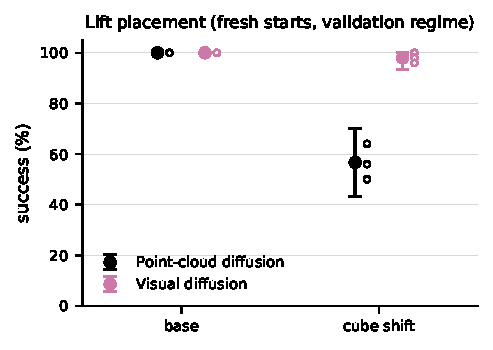
\includegraphics[width=0.8\linewidth]{generated/figures/level2.pdf}
\caption{Level~2: success of the point-cloud and RGB diffusion arms on the base starts and
under cube shift, with per-seed values.}
\label{fig:level2}
\end{figure}

\paragraph{Result.} The answer is no, in the opposite direction
(Table~\ref{tab:level2}, Figure~\ref{fig:level2}). Both arms succeed on every base start.
Under cube shift the point-cloud arm falls to \rf{l2.pcdiff.cube.succ}\,\% while the RGB arm
keeps \rf{l2.rgbdiff.cube.succ}\,\%; H5's difference is \rf{l2.h5.d}\,pp [\rf{l2.h5.lo},
\rf{l2.h5.hi}], separated, and the seed-level interval agrees ([\rf{sens.l2.h5.lo},
\rf{sens.l2.h5.hi}]). The point-cloud arm's own drop (\rf{l2.pcdiff.drop.d}\,pp) is separated
and the RGB arm's (\rf{l2.rgbdiff.drop.d}\,pp) is not. Because both arms are at the ceiling on
the base starts, the difference of drops equals H5 with its sign reversed and adds no
information. The point-cloud arm's failures are mostly misses next to the displaced cube and drops
(Table~\ref{tab:taxonomy}). On the held-out starts both arms succeed on every episode, so that
secondary comparison is uninformative; it is a check that the point-cloud arm works in
distribution, not evidence of equivalence.

\paragraph{What the result does and does not show.} H5 compares two complete policies, not
two modalities. Besides the input, the arms differ in their encoders (a ResNet-18 per camera,
\rf{rgb.enc.params} encoder parameters in total, against \rf{pc.enc.params} for the point
encoder), in augmentation (random crops for RGB, none for the cloud), and in the frame of the
input: the cloud is in absolute world coordinates, so shifting the cube moves its points to
coordinates the encoder never saw during training, whereas a convolutional encoder with
random crops may be more tolerant of translation (not tested here). The depth is noise-free and the calibration
exact. The result is therefore that \emph{this} point-cloud package, trained on
\rf{data.lift.train} demonstrations without augmentation, generalizes worse to unseen cube
positions than the matched RGB package. It does not test, and should not be read as
contradicting, the generalization results reported for DP3~\citep{ze2024dp3} under its own
design and tasks.

\section{Limitations and threats to validity}
\label{sec:limitations}

An independent audit of the code and the frozen files, run after every result was frozen,
produced the findings below; the full list, with evidence and the disposition of each, is in
\file{docs/AUDIT.md}. No finding changed a frozen file. Where a finding could be addressed from
committed data without a new rollout, it is addressed in this report and labelled.

\paragraph{Few seeds, and verdicts that depend on the method.} Each family has
\rf{proto.nseeds} training seeds. The seed-level sensitivity analysis
(Tables~\ref{tab:sens-main} and~\ref{tab:sens-rob}) changes
\rf{sens.l1.changed} of \rf{sens.l1.n} Level~1 verdicts, \rf{sens.rob.changed} of
\rf{sens.rob.n} robustness and ablation verdicts, and \rf{sens.ext.changed} of
\rf{sens.ext.n} verdicts of the two extensions; it is undefined for
\rf{sens.l1.undefined}, \rf{sens.rob.undefined} and \rf{sens.ext.undefined} of them because
the seeds do not vary. The separated Can H2 and H3 results, and several robustness
separations, are among the verdicts that change. The audit also found two verdicts that change
with the bootstrap's random seed. Of the \rf{sens.all.n} differences in the sensitivity
tables (the declared ones and one context row), \rf{sens.all.boundary} have a frozen interval
with a bound at exactly zero or of zero width; with \rf{proto.nstates} binary outcomes per seed the bootstrap distribution is
discrete, so these verdicts rest on ties. A policy that succeeds on all \rf{proto.nstates}
starts has a Wilson interval of [\rf{wilson.full.lo}, \rf{wilson.full.hi}]\,\%, so near the
ceiling the test separates only large differences.

\paragraph{Multiplicity.} No interval is adjusted for multiplicity. Each Level~1 task has
\rf{proto.ncomparisons} success comparisons and \rf{l1.lift.nlen} length comparisons, and
the robustness analyses report \rf{rob.lift.contrasts} (Lift) and \rf{rob.can.contrasts}
(Can) differences and contrasts. A Bonferroni correction within each analysis would remove several separations, among them
Can H2; the audit (\file{docs/AUDIT.md}, B-1 and B-6) gives the corrected intervals and the
count.

\paragraph{The diffusion sampler bounds its actions.} The sampler clips the predicted clean
action chunk to $[-1, 1]$ in min--max normalized space, so every diffusion action lies within
the range of the training actions on each dimension. The BC heads are clipped only to the
controller limits, which are wider. The audit found that in BC episodes that fail under perturbation most motion actions lie
outside the training range, while diffusion's never can. This is a correlation, not a shown
mechanism: the out-of-range actions begin only after a grasp is missed, BC-MLP leaves the
range on many base starts that it still solves, and BC-RNN rarely leaves it yet loses half
its success under the Lift arm offset. This bound is part of what H2-c compares: diffusion and BC-MLP-chunk differ in the
generative head \emph{and} in this output bound, so neither the Level~1 nor the robustness
differences between them isolate the generative model. Clamping BC outputs to the training
range would test this without retraining; it was not run in this report, because it would be
a new evaluation after the freeze.

\paragraph{Selection and its bias.} Validation success, which chose among \rf{train.K}
checkpoints and \rf{train.trials} trials, is optimistic: Table~\ref{tab:selection} shows it
beside success on the fresh base starts and on the held-out starts (for example BC-MLP on
Can: \rf{sel.can.bcmlp.val}\,\% on validation, \rf{l1.can.bcmlp.succ}\,\% held out).
Of the \rf{l1.bc.nruns} BC runs, \rf{l1.bc.first-ckpt} selected their first checkpoint, and two
diffusion runs their last, so the checkpoint grid may have been too coarse for BC and the
budget too short for those diffusion runs. In the RGB and Level~2 studies most checkpoints succeeded on
every validation start, so selection there was decided by tiny differences in episode length
and carries almost no information about the quantities those studies test; one RGB diffusion
run and one point-cloud run selected their final checkpoint. Each family had only
\rf{train.trials} tuning trials, and the extensions none, so no family is tuned to its best. Before the Lift
search space was committed, a short pipeline rehearsal (a few hundred training steps) had
evaluated the default and the higher-learning-rate configurations of BC-MLP and diffusion on
the validation suite; the higher learning rate was later chosen for Lift diffusion. The trial
list was the same for every family, but BC-RNN and BC-MLP-chunk had no such early look.

\paragraph{One rollout per start.} With $R = \rf{proto.repeats}$, a start's difficulty and the
diffusion noise drawn on it are confounded, so diffusion's interval mixes policy stochasticity
with start difficulty, unlike the deterministic BC families (KI-028).

\paragraph{Reuse of starts across studies.} The same \rf{proto.nstates} Lift held-out starts
served the Level~1 test, the RGB test and the Level~2 held-out check, and the robustness base
and cube-shift starts served both H4 and H5. No model, checkpoint or configuration was ever
selected on them. However, the three studies were designed in sequence and later designs were
informed by earlier outcomes on these starts: H5's primary set was chosen after the Level~1
robustness and RGB held-out results were known. The Level~2 held-out comparison, with both
arms at the ceiling, could not have favoured the point-cloud arm and is a replication-type
check, not a test.

\paragraph{Scale of the diffusion policy.} The diffusion family was matched to BC in
parameters (about a million) and in its optimizer recipe. robomimic's default U-Net is wider
and deeper and is trained with a warm-up cosine schedule, so these results speak to
diffusion at this scale and recipe only.

\paragraph{In-distribution starts.} The evaluation starts come from the same reset
distribution as the demonstrations; on Lift each start lies within a few millimetres of a
demonstration start (KI-011), so Lift held-out success measures in-distribution performance.
Open-loop replay of the Can demonstrations diverges at contacts by several centimetres
(KI-004), so the simulator reproduces the recorded dynamics only approximately.

\paragraph{Privilege, features and platform.} Every Level~1 result uses exact object poses.
The Can input recomputes the gripper-to-object vector from the current step, unlike
robomimic's stored feature, so Can numbers are not comparable with robomimic's. The data are
the robosuite~v1.5 repackaging of the robomimic datasets, so no number here should be compared
with the original benchmark. All rollouts ran in simulation on one platform. Our success
predicate is evaluated on the current step's kinematics, while robosuite's own predicate reads
the previous substep; in a small fraction of episodes ours fires one control step earlier,
which shifts first-success steps but not success. The point cloud uses noise-free depth, exact
camera calibration and a crop box whose lower edge removes the table at its known height.

\paragraph{Declared quantities not reported, and quantities not declared.} The protocol's
secondary metrics (gripper sign changes, action smoothness) were computed per episode but
never aggregated by the frozen analysis; Table~\ref{tab:secondary} reports them post hoc. The diffusion-specific plan-diversity metric was measured only in a pilot and is not
reported, and the point-cloud throughput listed in the Level~2 freeze is not in its results.
Validation success at every checkpoint, declared for the RGB study, and the point-cloud
per-checkpoint rates listed in the Level~2 freeze are in the committed selection files but
not in this report. The H4 analysis
compares four of the six family pairs, a choice fixed in code before any robustness rollout.
The optional DiT and GMM-BC families and the Square task were not run, to stay within the
project's time and compute budget; the declared hypotheses did not depend on them.

\paragraph{Analysis code, records and cost figures.} The Level~1 analysis script was
hash-frozen; the robustness, RGB and Level~2 analysis scripts were not, and each received a
small fix after its data existed. The fixes touched input reading and training-time accounting
only, not pairing, resampling or which evaluations enter. The validation summaries of one RGB
training run were recorded from a working tree with uncommitted changes; the next commit
changed only documentation, logs and reports, and the frozen code hashes match. The Level~2 analysis misreported one training time (KI-049), and one RGB run's
hours leave out a preempted attempt (Table~\ref{tab:cost}). Billed amounts are Modal's usage
report at list price before credits, not invoices; one early approval allowed one GPU probe
and two probe launches ran before the owner amended it.

\paragraph{Scope of the claims.} The comparison covers two tasks, privileged state for
Level~1, \rf{data.lift.train} training demonstrations per task from one operator channel, one training budget and one
platform. Within that scope the evidence supports an advantage of BC-RNN over BC-MLP on Lift under
both interval methods and on Can under the preregistered bootstrap only, gives no evidence
that a diffusion head adds to a deterministic head with the same horizons, and shows that our point-cloud policy generalizes worse than our RGB
policy to unseen cube positions. It supports no claim about real robots, other tasks, larger
datasets or DP3 itself.

\section{Conclusion}
\label{sec:conclusion}

Under one preregistered protocol, with matched inputs, parameter counts, budgets and tuning,
a diffusion policy over action chunks did not outperform a deterministic MLP that sees the
same observation window and predicts the same chunks, on either Lift or Can. Its advantage
over a one-step MLP on Can is not separated from that of an LSTM or of the chunked MLP, so
the data give no evidence for the generative model beyond temporal context on these tasks,
and even the separation from the one-step MLP depends on how the uncertainty over three seeds
is computed. Diffusion was the most robust family to a large joint offset on Lift; on Can its
drop was not separated from the chunked MLP's, and part of its robustness may come from its
sampler's bound on its actions. It cost more than an order of
magnitude more training and inference time than the chunked MLP. With images, visual BC and
visual diffusion both reach the Lift ceiling, and our DP3-inspired point-cloud policy, which
uses world-frame coordinates and no augmentation, generalized clearly worse than the matched
RGB policy to unseen cube positions.

The most useful next steps follow from the limitations: more training seeds, harder tasks
that are not saturated, more than one rollout per start, a BC baseline with the same action
bound as the diffusion sampler, and a point-cloud arm with augmentation or an object-centred
frame. Each would need its own preregistration and freeze before it is run.


\bibliographystyle{plainnat}
\bibliography{references}

\clearpage
\appendix
\section{Reproducibility}
\label{app:repro}

\paragraph{Software and data.} Simulation: robosuite \rf{ver.robosuite} (commit
\texttt{\rf{ver.robosuite.commit}}), MuJoCo \rf{ver.mujoco}; learning: robomimic
\rf{ver.robomimic} (commit \texttt{\rf{ver.robomimic.commit}}), PyTorch \rf{ver.torch}, NumPy
\rf{ver.numpy}, diffusers \rf{ver.diffusers} (scheduler reference only); Python
\rf{ver.python}. All versions are pinned in the repository's \file{uv.lock}. Every reported
rollout ran in the container image \code{sha256:}\rf{plat.image}. The demonstrations are the
Hugging Face \code{robomimic/robomimic_datasets} files at revision \rf{data.hf.revision}, with
the SHA-256 prefixes of Section~\ref{sec:setup}, released under the \rf{data.license} license
according to the dataset card; \code{make download} fetches and verifies them, and they are
not redistributed. The RoboForge code is released under the license Apache-2.0; robosuite,
robomimic and MuJoCo keep their own licenses.

\paragraph{Splits and initial states.} The training and validation episode IDs are in
\file{data/splits/lift_ph.json} and \file{data/splits/can_ph.json} (Table~\ref{tab:sources}).
Each evaluation suite is a manifest with per-state hashes under
\file{data/eval_states/<task>/<suite>/}; the held-out manifests' content SHA-256 prefixes are
\texttt{\rf{l1.lift.heldout.manifest}} (Lift) and \texttt{\rf{l1.can.heldout.manifest}} (Can), as
recorded in the Level~1 freeze. The robustness sets are derived deterministically from the
base starts by \file{configs/eval/robustness.yaml}.

\paragraph{Frozen results.} The Level~1 held-out analysis ran at commit \texttt{\rf{l1.git}},
the robustness analysis at \texttt{\rf{rob.git}}, the RGB analysis at \texttt{\rf{rgb.git}} and the
Level~2 analysis at \texttt{\rf{l2.git}}. Each study's freeze document, committed before its
first governed run, lists the SHA-256 of every code and configuration file it depends on; a
repository check compares those hashes with the working tree. Table~\ref{tab:sources} lists
every frozen file this report reads, with its SHA-256 prefix. The evaluation summaries that a
results file cites are read only after their hash matches the one recorded in that file.

\paragraph{Regenerating this report.} Every table, figure and number in the text is generated
from those files by \code{scripts/paper_assets.py}; the prose uses only generated macros. The
generator never reads the interactive viewer's summaries or the training-run directories.
\begin{itemize}
\item \code{make paper-assets} regenerates \file{paper/generated/}, including an index with
  the SHA-256 of every output and of every source it read.
\item \code{make paper-check} confirms that the committed generated files equal a fresh build
  byte for byte and lints the sections for typed numbers, placeholders and undefined macros.
\item \code{make paper-bibcheck} resolves every DOI and arXiv identifier of the bibliography
  and compares titles and first authors (it needs network access).
\item \code{make paper} builds \file{paper/main.pdf} with Tectonic from its cached bundle,
  without network access, and with a fixed source date so that the PDF is byte-identical
  across builds.
\end{itemize}

\paragraph{Commands and budgets.} Training runs through \code{make train} and the suite
orchestrator \code{make suite} with the committed plans
(\file{configs/experiments/level1_core_lift.yaml} and \file{level1_core_can.yaml}): every
run \rf{train.steps} steps, a checkpoint every \rf{train.ckpt} steps, every checkpoint on the
\rf{proto.nstates} validation starts. Every rollout is capped at the \rf{proto.horizon}-step
horizon. The held-out tests and their analyses (\code{make eval-final},
\code{make analyze-final}, \code{make rgb-heldout}, \code{make pc-placement},
\code{make pc-heldout}, \code{make level2-analyze}) each ran once, after the freeze that governs it was
committed, and must never be rerun. Each paid GPU launch was limited to one
hour and ran under a committed approval with a dollar cap (Table~\ref{tab:spend}).

\paragraph{What is not redistributed.} Trained checkpoints, rollout records and per-episode
arrays live in the training-run directories, which are not part of the repository. The
committed evaluation summaries, selections and analyses suffice to regenerate every number
here, but not to re-run a policy without retraining it. Retraining follows the committed
configurations; Level~1 runs train on a CPU, and the RGB and Level~2 runs need one NVIDIA L4
GPU.

\begin{table}[p]
\centering\scriptsize
\caption{Frozen sources read by the report generator, with their SHA-256 prefixes.}
\label{tab:sources}
% Generated by scripts/paper_assets.py (DECISIONS D-094). Do not edit.
% Sources (path sha256):
%   configs/models/diffusion_unet.yaml ca181c22a4af5499a67066fe2d78c06aeff5a889212ad3cceed7265fc8228bbf
%   configs/models/pointcloud/diffusion_dp3_lift.yaml b56f515dfd861568c27d5c89ebaa9878bb87452a634daebf776f58174bfe802a
%   reports/compute/cost_ledger.jsonl a4f92b9f1f4ae3708bacea7a34946b3a51705205b1fc4e4a2666096f3ba40578
%   reports/data_audit.json 1812ad718b506247ab10361d760652b6db1286f5758a05bfb847932695dbaa21
%   data/manifests/robomimic_v1.5_ph.json 34987db82f9a60a0da017ca5169eeae2214fd590505786063f59b85226f89188
%   docs/FINAL_TEST_FREEZE.md 6a3c6874c4bc1857efe46ccb05c0a1fa68247671fc9a96f5f54ce079aa9153e9
%   reports/session7/results/results.json b8b097c38765c588711615917e3cfd5be6847e63083ddebe92f0f1488672408c
%   reports/session7/robustness/analysis.json 8cca66a8a8a8cecf0b734355167936e81983c821c625a23456523365409c9451
%   reports/session7/results/taxonomy.json 7a71518171c8303cc00e357626ba66c64902b3d0e179ce82ba41504c2d6516b8
%   reports/session9/level2_results/ERRATA.md 280974a994408a6f7d3683788561f0f6c05de90f4eccf8d7b1636dd90fabca31
%   docs/LEVEL2_EXPERIMENT_FREEZE.md ffe5a03e98714465acf8655c281dea653197835f4e218cfb97a1ba6173589d81
%   reports/session9/level2_results/results.json 1d33c975e49df907a6543b17e0cf36d047f7b5ce11aa69a355313e146c22571e
%   logs/session9/pc_train/launch_records/train_gpu_pc_20261109T130430.result.json 0ea097359ba49b375e3ce53199435b771e9c3253e1e039baa62f71a003e2a737
%   reports/session4/param_counts.json 0ec7b26a0a329737cc0b18a968f5276d7130a5f66614305985505a16532486cb
%   configs/experiments/level1_core_can.yaml 881b4fb7fd72a33866ad4924db3b72cbe4270a212b03a8cc958efc6ba8a89e3c
%   configs/experiments/level2_pointcloud.yaml d91a546e1774779b27a16edbd5f33b0a2d4c11e6d68c71c13e2dff7e0a3e5c9d
%   configs/experiments/level1_core_lift.yaml d3de6cbcb14bcda15023a6526c6e3ba8cafb0b37d8692c5f8b6fcba871cfad3f
%   configs/eval/platform.yaml a152eb41157f4b4dc6f9f1767c79d2e32c6df9b9a351430ca1dfe7af24eb2fd5
%   docs/RGB_EXPERIMENT_FREEZE.md 47e7cb8ee70743dbcc6a0295a92a7462a2309870aebb3eda19060ca0e0ac385f
%   reports/session8/rgb_results/results.json 57663b81aafc70e9c1d850322b6bb1b894f7dad0d082976b1f546475a601390e
%   configs/eval/robustness.yaml cfa933cac8719e329c8159d2ccfa18ba2fcd58cc412b9ef65707e3e918a11d1f
%   data/splits/can_ph.json 754967ce665fca0084d3657e8e2d511db43d35f218d517c0bd15c93c17e75115
%   data/splits/lift_ph.json e36d89afb6d0704aa8536e23696fe30f894243ed80030e568f9a0ba3fd3a5273
%   reports/session7/suite/level1_core_can.json 213bb2c00de1a6f6631d431cb6114d2c7776ba75fc47cbc59c963ebd9adb8629
%   reports/session6/suite/level1_core_lift.json 45c28837c1fd507946856f8acc3d9a376da4ce86de1d5222ea0a08b82c757faa
%   uv.lock 327eaa2ea05a4e8fa46d8ed717ae4c7f5bcfa9a4069edac31b778d6b42ac5ca9
\begin{tabular}{p{0.42\linewidth}lp{0.36\linewidth}}
\toprule
Source & SHA-256 (prefix) & Content \\
\midrule
\texttt{reports/\allowbreak{}session7/\allowbreak{}results/\allowbreak{}results.json} & \texttt{b8b097c38765c588} & Level 1 held-out analysis (frozen, run once) \\
\texttt{reports/\allowbreak{}session7/\allowbreak{}results/\allowbreak{}taxonomy.json} & \texttt{7a71518171c8303c} & Level 1 held-out failure taxonomy per episode \\
\texttt{reports/\allowbreak{}session7/\allowbreak{}robustness/\allowbreak{}analysis.json} & \texttt{8cca66a8a8a8cecf} & Level 1 robustness and ablation analysis (validation regime) \\
\texttt{reports/\allowbreak{}session8/\allowbreak{}rgb\_results/\allowbreak{}results.json} & \texttt{57663b81aafc70e9} & RGB study held-out analysis (frozen, run once) \\
\texttt{reports/\allowbreak{}session9/\allowbreak{}level2\_results/\allowbreak{}results.json} & \texttt{1d33c975e49df907} & Level 2 analysis, placement (H5) and held-out (frozen, run once) \\
\texttt{reports/\allowbreak{}session9/\allowbreak{}level2\_results/\allowbreak{}ERRATA.md} & \texttt{280974a994408a6f} & Level 2 erratum (KNOWN\_ISSUES KI-049), cited beside the row it corrects \\
\texttt{logs/\allowbreak{}session9/\allowbreak{}pc\_train/\allowbreak{}launch\_records/\allowbreak{}train\_gpu\_pc\_20261109T130430.result.json} & \texttt{0ea097359ba49b37} & Level 2 seed 0 completing launch record (KI-049 correction) \\
\texttt{reports/\allowbreak{}compute/\allowbreak{}cost\_ledger.jsonl} & \texttt{a4f92b9f1f4ae370} & Machine-readable cost ledger (launch, result and billing events) \\
\texttt{docs/\allowbreak{}FINAL\_TEST\_FREEZE.md} & \texttt{6a3c6874c4bc1857} & Level 1 held-out freeze (machine-readable block) \\
\texttt{docs/\allowbreak{}RGB\_EXPERIMENT\_FREEZE.md} & \texttt{47e7cb8ee70743db} & RGB study freeze \\
\texttt{docs/\allowbreak{}LEVEL2\_EXPERIMENT\_FREEZE.md} & \texttt{ffe5a03e98714465} & Level 2 freeze \\
\texttt{data/\allowbreak{}manifests/\allowbreak{}robomimic\_v1.5\_ph.json} & \texttt{34987db82f9a60a0} & Dataset manifest (robomimic v1.5 PH, Hugging Face revision, SHA-256) \\
\texttt{data/\allowbreak{}splits/\allowbreak{}lift\_ph.json} & \texttt{e36d89afb6d0704a} & Lift demonstration split \\
\texttt{data/\allowbreak{}splits/\allowbreak{}can\_ph.json} & \texttt{754967ce665fca00} & Can demonstration split \\
\texttt{reports/\allowbreak{}data\_audit.json} & \texttt{1812ad718b506247} & Data audit (episode lengths, control period, action statistics) \\
\texttt{reports/\allowbreak{}session4/\allowbreak{}param\_counts.json} & \texttt{0ec7b26a0a329737} & Exact parameter counts of the Level 1 families \\
\texttt{configs/\allowbreak{}eval/\allowbreak{}robustness.yaml} & \texttt{cfa933cac8719e32} & Preregistered robustness sets (RESEARCH\_PROTOCOL §14) \\
\texttt{configs/\allowbreak{}eval/\allowbreak{}platform.yaml} & \texttt{a152eb41157f4b4d} & Canonical evaluation platform \\
\texttt{configs/\allowbreak{}experiments/\allowbreak{}level1\_core\_lift.yaml} & \texttt{d3de6cbcb14bcda1} & Level 1 Lift suite plan (budget, tuning trials) \\
\texttt{configs/\allowbreak{}experiments/\allowbreak{}level1\_core\_can.yaml} & \texttt{881b4fb7fd72a338} & Level 1 Can suite plan (budget, tuning trials) \\
\texttt{configs/\allowbreak{}experiments/\allowbreak{}level2\_pointcloud.yaml} & \texttt{d91a546e1774779b} & Level 2 plan \\
\texttt{configs/\allowbreak{}models/\allowbreak{}diffusion\_unet.yaml} & \texttt{ca181c22a4af5499} & Level 1 diffusion configuration (base; trials override the optimizer only) \\
\texttt{configs/\allowbreak{}models/\allowbreak{}pointcloud/\allowbreak{}diffusion\_dp3\_lift.yaml} & \texttt{b56f515dfd861568} & Level 2 point-cloud arm configuration \\
\texttt{reports/\allowbreak{}session6/\allowbreak{}suite/\allowbreak{}level1\_core\_lift.json} & \texttt{45c28837c1fd5079} & Level 1 Lift suite summary (validation selections, development numbers) \\
\texttt{reports/\allowbreak{}session7/\allowbreak{}suite/\allowbreak{}level1\_core\_can.json} & \texttt{213bb2c00de1a6f6} & Level 1 Can suite summary (validation selections, development numbers) \\
\texttt{uv.lock} & \texttt{327eaa2ea05a4e8f} & Locked Python environment (package versions) \\
\texttt{reports/\allowbreak{}session10/\allowbreak{}observatory/\allowbreak{}verification/\allowbreak{}lift-\allowbreak{}diffusion\_unet-\allowbreak{}s0-\allowbreak{}lift\_final\_test\_0000\_t021\_frontview\_rgb.png} & \texttt{b6a165f72de1fb92} & Lift, diffusion seed 0, held-out start 0, frame 21: MuJoCo frontview render of the recorded state (Session 10 viewer-verification reference) \\
\texttt{reports/\allowbreak{}session10/\allowbreak{}observatory/\allowbreak{}verification/\allowbreak{}can-\allowbreak{}diffusion\_unet-\allowbreak{}s0-\allowbreak{}can\_final\_test\_0000\_t060\_frontview\_rgb.png} & \texttt{149b860b17a2eca4} & Can, diffusion seed 0, held-out start 0, frame 60: MuJoCo frontview render of the recorded state (Session 10 viewer-verification reference) \\
\texttt{reports/\allowbreak{}session9/\allowbreak{}pc\_feasibility/\allowbreak{}linux-\allowbreak{}aarch64-\allowbreak{}container-\allowbreak{}1f685638f28c/\allowbreak{}lift\_overlay\_demo\_0\_t029.png} & \texttt{fe163485aaccd6a2} & Lift demo 0, t = 29: the 512 sampled cloud points projected on the frontview and agentview frames (Session 9 feasibility, canonical container) \\
\texttt{reports/\allowbreak{}session7/\allowbreak{}heldout/\allowbreak{}} (26 files) & per file & Level 1 held-out evaluation summaries, each read only after its SHA-256 equals the one recorded in the Level 1 results file (D-096) \\
\bottomrule
\end{tabular}

\end{table}

\section{Additional tables}
\label{app:tables}

\begin{table}[p]
\centering\scriptsize
\caption{Level~1 held-out results per selected checkpoint: training step, successes, Wilson
\rf{proto.level}\,\% interval and mean first-success step.}
\label{tab:checkpoints}
% Generated by scripts/paper_assets.py (DECISIONS D-094). Do not edit.
% Sources (path sha256):
%   reports/session7/results/results.json b8b097c38765c588711615917e3cfd5be6847e63083ddebe92f0f1488672408c
\begin{tabular}{llrrrrr}
\toprule
Family & Seed & Step & $k/n$ & Wilson 95\,\% & First success & Errors \\
\midrule
\multicolumn{7}{l}{\emph{Lift}} \\
BC-MLP & 0 & 15,000 & 44/50 & [76.2, 94.4] & 54.2 & 0 \\
BC-MLP & 1 & 5,000 & 46/50 & [81.2, 96.8] & 48.7 & 0 \\
BC-MLP & 2 & 5,000 & 46/50 & [81.2, 96.8] & 47.3 & 0 \\
BC-RNN & 0 & 15,000 & 50/50 & [92.9, 100.0] & 43.5 & 0 \\
BC-RNN & 1 & 10,000 & 50/50 & [92.9, 100.0] & 42.3 & 0 \\
BC-RNN & 2 & 5,000 & 50/50 & [92.9, 100.0] & 42.5 & 0 \\
BC-MLP-chunk & 0 & 15,000 & 49/50 & [89.5, 99.6] & 45.0 & 0 \\
BC-MLP-chunk & 1 & 5,000 & 50/50 & [92.9, 100.0] & 43.3 & 0 \\
BC-MLP-chunk & 2 & 10,000 & 48/50 & [86.5, 98.9] & 43.3 & 0 \\
Diffusion U-Net & 0 & 100,000 & 49/50 & [89.5, 99.6] & 44.9 & 0 \\
Diffusion U-Net & 1 & 95,000 & 48/50 & [86.5, 98.9] & 44.1 & 0 \\
Diffusion U-Net & 2 & 80,000 & 49/50 & [89.5, 99.6] & 43.9 & 0 \\
Random (uniform) & -- & -- & 0/50 & [0.0, 7.1] & -- & 0 \\
\multicolumn{7}{l}{\emph{Can}} \\
BC-MLP & 0 & 55,000 & 34/50 & [54.2, 79.2] & 121.4 & 0 \\
BC-MLP & 1 & 15,000 & 44/50 & [76.2, 94.4] & 116.3 & 0 \\
BC-MLP & 2 & 55,000 & 37/50 & [60.4, 84.1] & 117.4 & 0 \\
BC-RNN & 0 & 30,000 & 46/50 & [81.2, 96.8] & 114.2 & 0 \\
BC-RNN & 1 & 25,000 & 50/50 & [92.9, 100.0] & 118.3 & 0 \\
BC-RNN & 2 & 35,000 & 48/50 & [86.5, 98.9] & 110.6 & 0 \\
BC-MLP-chunk & 0 & 95,000 & 48/50 & [86.5, 98.9] & 104.6 & 0 \\
BC-MLP-chunk & 1 & 85,000 & 46/50 & [81.2, 96.8] & 106.2 & 0 \\
BC-MLP-chunk & 2 & 30,000 & 50/50 & [92.9, 100.0] & 109.2 & 0 \\
Diffusion U-Net & 0 & 65,000 & 46/50 & [81.2, 96.8] & 115.3 & 0 \\
Diffusion U-Net & 1 & 100,000 & 49/50 & [89.5, 99.6] & 114.3 & 0 \\
Diffusion U-Net & 2 & 90,000 & 48/50 & [86.5, 98.9] & 114.2 & 0 \\
Random (uniform) & -- & -- & 0/50 & [0.0, 7.1] & -- & 0 \\
\bottomrule
\end{tabular}

\end{table}

\begin{table}[p]
\centering\scriptsize
\caption{Validation success of the selected checkpoints beside their success on the fresh
robustness base starts and on the held-out starts (\%). Validation chose the checkpoints, so
it is biased upward.}
\label{tab:selection}
% Generated by scripts/paper_assets.py (DECISIONS D-094). Do not edit.
% Sources (path sha256):
%   reports/session7/results/results.json b8b097c38765c588711615917e3cfd5be6847e63083ddebe92f0f1488672408c
%   reports/session7/robustness/analysis.json 8cca66a8a8a8cecf0b734355167936e81983c821c625a23456523365409c9451
%   reports/session7/suite/level1_core_can.json 213bb2c00de1a6f6631d431cb6114d2c7776ba75fc47cbc59c963ebd9adb8629
%   reports/session6/suite/level1_core_lift.json 45c28837c1fd507946856f8acc3d9a376da4ce86de1d5222ea0a08b82c757faa
\begin{tabular}{lrrrrrr}
\toprule
Family & Lift validation & Lift fresh base & Lift held-out & Can validation & Can fresh base & Can held-out \\
\midrule
BC-MLP & 97.3 & 98.0 & 90.7 & 82.7 & 69.3 & 76.7 \\
BC-RNN & 100.0 & 100.0 & 100.0 & 99.3 & 96.7 & 96.0 \\
BC-MLP-chunk & 99.3 & 100.0 & 98.0 & 100.0 & 95.3 & 96.0 \\
Diffusion U-Net & 100.0 & 99.3 & 97.3 & 98.7 & 92.0 & 95.3 \\
\bottomrule
\end{tabular}

\end{table}

\begin{table}[p]
\centering\scriptsize
\caption{H4: per-family drops and between-family differences on the perturbation sets, with
the bootstrap \rf{proto.level}\,\% interval.}
\label{tab:contrasts}
% Generated by scripts/paper_assets.py (DECISIONS D-094). Do not edit.
% Sources (path sha256):
%   reports/session7/robustness/analysis.json 8cca66a8a8a8cecf0b734355167936e81983c821c625a23456523365409c9451
\begin{tabular}{lrl}
\toprule
Contrast & Estimate (pp) [95\,\% CI] & Outcome \\
\midrule
\multicolumn{3}{l}{\emph{Lift}} \\
drop of BC-MLP, base $-$ cube shift & \ensuremath{+}45.3 [\ensuremath{+}30.7, \ensuremath{+}60.7] & separated (\ensuremath{+}) \\
drop of BC-RNN, base $-$ cube shift & \ensuremath{+}4.0 [\ensuremath{+}0.0, \ensuremath{+}12.0] & not separated \\
drop of BC-MLP-chunk, base $-$ cube shift & \ensuremath{+}45.3 [\ensuremath{+}24.7, \ensuremath{+}66.7] & separated (\ensuremath{+}) \\
drop of Diffusion U-Net, base $-$ cube shift & \ensuremath{+}14.0 [\ensuremath{+}6.0, \ensuremath{+}22.7] & separated (\ensuremath{+}) \\
drop of BC-MLP, base $-$ arm offset & \ensuremath{+}75.3 [\ensuremath{+}64.7, \ensuremath{+}85.3] & separated (\ensuremath{+}) \\
drop of BC-RNN, base $-$ arm offset & \ensuremath{+}50.0 [\ensuremath{+}36.0, \ensuremath{+}64.0] & separated (\ensuremath{+}) \\
drop of BC-MLP-chunk, base $-$ arm offset & \ensuremath{+}51.3 [\ensuremath{+}38.7, \ensuremath{+}64.0] & separated (\ensuremath{+}) \\
drop of Diffusion U-Net, base $-$ arm offset & \ensuremath{+}11.3 [\ensuremath{+}2.7, \ensuremath{+}20.7] & separated (\ensuremath{+}) \\
Diffusion U-Net $-$ BC-MLP on cube shift & \ensuremath{+}32.7 [\ensuremath{+}14.7, \ensuremath{+}50.7] & separated (\ensuremath{+}) \\
Diffusion U-Net $-$ BC-RNN on cube shift & \ensuremath{-}10.7 [\ensuremath{-}21.3, \ensuremath{+}0.0] & not separated \\
Diffusion U-Net $-$ BC-MLP-chunk on cube shift & \ensuremath{+}30.7 [\ensuremath{+}9.3, \ensuremath{+}52.7] & separated (\ensuremath{+}) \\
BC-RNN $-$ BC-MLP on cube shift & \ensuremath{+}43.3 [\ensuremath{+}26.0, \ensuremath{+}62.0] & separated (\ensuremath{+}) \\
Diffusion U-Net $-$ BC-MLP on arm offset & \ensuremath{+}65.3 [\ensuremath{+}52.0, \ensuremath{+}78.0] & separated (\ensuremath{+}) \\
Diffusion U-Net $-$ BC-RNN on arm offset & \ensuremath{+}38.0 [\ensuremath{+}24.0, \ensuremath{+}52.0] & separated (\ensuremath{+}) \\
Diffusion U-Net $-$ BC-MLP-chunk on arm offset & \ensuremath{+}39.3 [\ensuremath{+}25.3, \ensuremath{+}53.3] & separated (\ensuremath{+}) \\
BC-RNN $-$ BC-MLP on arm offset & \ensuremath{+}27.3 [\ensuremath{+}13.3, \ensuremath{+}42.7] & separated (\ensuremath{+}) \\
drop Diffusion U-Net $-$ drop BC-MLP on cube shift & \ensuremath{-}31.3 [\ensuremath{-}48.0, \ensuremath{-}15.3] & separated (\ensuremath{-}) \\
drop Diffusion U-Net $-$ drop BC-RNN on cube shift & \ensuremath{+}10.0 [\ensuremath{-}0.7, \ensuremath{+}20.7] & not separated \\
drop Diffusion U-Net $-$ drop BC-MLP-chunk on cube shift & \ensuremath{-}31.3 [\ensuremath{-}54.0, \ensuremath{-}10.0] & separated (\ensuremath{-}) \\
drop BC-RNN $-$ drop BC-MLP on cube shift & \ensuremath{-}41.3 [\ensuremath{-}58.0, \ensuremath{-}25.3] & separated (\ensuremath{-}) \\
drop Diffusion U-Net $-$ drop BC-MLP on arm offset & \ensuremath{-}64.0 [\ensuremath{-}76.7, \ensuremath{-}50.7] & separated (\ensuremath{-}) \\
drop Diffusion U-Net $-$ drop BC-RNN on arm offset & \ensuremath{-}38.7 [\ensuremath{-}53.3, \ensuremath{-}24.0] & separated (\ensuremath{-}) \\
drop Diffusion U-Net $-$ drop BC-MLP-chunk on arm offset & \ensuremath{-}40.0 [\ensuremath{-}54.0, \ensuremath{-}26.0] & separated (\ensuremath{-}) \\
drop BC-RNN $-$ drop BC-MLP on arm offset & \ensuremath{-}25.3 [\ensuremath{-}40.0, \ensuremath{-}11.3] & separated (\ensuremath{-}) \\
\multicolumn{3}{l}{\emph{Can}} \\
drop of BC-MLP, base $-$ arm offset & \ensuremath{+}39.3 [\ensuremath{+}26.0, \ensuremath{+}52.0] & separated (\ensuremath{+}) \\
drop of BC-RNN, base $-$ arm offset & \ensuremath{+}43.3 [\ensuremath{+}30.0, \ensuremath{+}56.7] & separated (\ensuremath{+}) \\
drop of BC-MLP-chunk, base $-$ arm offset & \ensuremath{+}16.0 [\ensuremath{+}6.0, \ensuremath{+}28.0] & separated (\ensuremath{+}) \\
drop of Diffusion U-Net, base $-$ arm offset & \ensuremath{+}20.7 [\ensuremath{+}8.0, \ensuremath{+}34.0] & separated (\ensuremath{+}) \\
Diffusion U-Net $-$ BC-MLP on arm offset & \ensuremath{+}41.3 [\ensuremath{+}26.0, \ensuremath{+}57.3] & separated (\ensuremath{+}) \\
Diffusion U-Net $-$ BC-RNN on arm offset & \ensuremath{+}18.0 [\ensuremath{+}3.3, \ensuremath{+}32.7] & separated (\ensuremath{+}) \\
Diffusion U-Net $-$ BC-MLP-chunk on arm offset & \ensuremath{-}8.0 [\ensuremath{-}23.3, \ensuremath{+}8.7] & not separated \\
BC-RNN $-$ BC-MLP on arm offset & \ensuremath{+}23.3 [\ensuremath{+}8.7, \ensuremath{+}38.7] & separated (\ensuremath{+}) \\
drop Diffusion U-Net $-$ drop BC-MLP on arm offset & \ensuremath{-}18.7 [\ensuremath{-}36.0, \ensuremath{-}0.7] & separated (\ensuremath{-}) \\
drop Diffusion U-Net $-$ drop BC-RNN on arm offset & \ensuremath{-}22.7 [\ensuremath{-}39.3, \ensuremath{-}5.3] & separated (\ensuremath{-}) \\
drop Diffusion U-Net $-$ drop BC-MLP-chunk on arm offset & \ensuremath{+}4.7 [\ensuremath{-}10.7, \ensuremath{+}20.7] & not separated \\
drop BC-RNN $-$ drop BC-MLP on arm offset & \ensuremath{+}4.0 [\ensuremath{-}12.7, \ensuremath{+}21.3] & not separated \\
\bottomrule
\end{tabular}

\end{table}

\begin{table}[p]
\centering\scriptsize
\caption{Sensitivity analysis, not preregistered (D-095): every declared difference of the
held-out studies with its frozen bootstrap interval and a seed-level $t$ interval
(degrees of freedom in brackets). $\ast$: the seed-level verdict differs from the frozen
one. The frozen verdict is the reported result.}
\label{tab:sens-main}
\resizebox{\linewidth}{!}{% Generated by scripts/paper_assets.py (DECISIONS D-094). Do not edit.
% Sources (path sha256):
%   reports/session7/results/results.json b8b097c38765c588711615917e3cfd5be6847e63083ddebe92f0f1488672408c
%   reports/session7/robustness/analysis.json 8cca66a8a8a8cecf0b734355167936e81983c821c625a23456523365409c9451
%   reports/session9/level2_results/results.json 1d33c975e49df907a6543b17e0cf36d047f7b5ce11aa69a355313e146c22571e
%   reports/session8/rgb_results/results.json 57663b81aafc70e9c1d850322b6bb1b894f7dad0d082976b1f546475a601390e
\begin{tabular}{llll}
\toprule
Comparison & Frozen bootstrap (pp) & Seed-level $t$ (pp, df) & \\
\midrule
\multicolumn{4}{l}{\emph{Level 1 held-out, Lift}} \\
H1: BC-MLP $-$ Random (uniform) & \ensuremath{+}90.7 [\ensuremath{+}83.3, \ensuremath{+}96.7], separated (\ensuremath{+}) & [\ensuremath{+}84.9, \ensuremath{+}96.4] (2.0), separated (\ensuremath{+}) &  \\
H1: BC-RNN $-$ Random (uniform) & \ensuremath{+}100.0 [\ensuremath{+}100.0, \ensuremath{+}100.0], separated (\ensuremath{+}) & undefined (no seed variance) &  \\
H1: BC-MLP-chunk $-$ Random (uniform) & \ensuremath{+}98.0 [\ensuremath{+}94.0, \ensuremath{+}100.0], separated (\ensuremath{+}) & [\ensuremath{+}93.0, \ensuremath{+}103.0] (2.0), separated (\ensuremath{+}) &  \\
H1: Diffusion $-$ Random (uniform) & \ensuremath{+}97.3 [\ensuremath{+}93.3, \ensuremath{+}100.0], separated (\ensuremath{+}) & [\ensuremath{+}94.5, \ensuremath{+}100.2] (2.0), separated (\ensuremath{+}) &  \\
H2: Diffusion $-$ BC-MLP & \ensuremath{+}6.7 [\ensuremath{-}0.7, \ensuremath{+}14.7], not separated & [\ensuremath{+}1.9, \ensuremath{+}11.5] (2.9), separated (\ensuremath{+}) & $\ast$ \\
H2: Diffusion $-$ BC-RNN & \ensuremath{-}2.7 [\ensuremath{-}6.7, \ensuremath{+}0.0], not separated & [\ensuremath{-}5.5, \ensuremath{+}0.2] (2.0), not separated &  \\
H2-c: Diffusion $-$ BC-MLP-chunk & \ensuremath{-}0.7 [\ensuremath{-}5.3, \ensuremath{+}4.7], not separated & [\ensuremath{-}4.8, \ensuremath{+}3.4] (3.2), not separated &  \\
H3: BC-RNN $-$ BC-MLP & \ensuremath{+}9.3 [\ensuremath{+}3.3, \ensuremath{+}16.7], separated (\ensuremath{+}) & [\ensuremath{+}3.6, \ensuremath{+}15.1] (2.0), separated (\ensuremath{+}) &  \\
\addlinespace
\multicolumn{4}{l}{\emph{Level 1 held-out, Can}} \\
H1: BC-MLP $-$ Random (uniform) & \ensuremath{+}76.7 [\ensuremath{+}62.7, \ensuremath{+}90.0], separated (\ensuremath{+}) & [\ensuremath{+}51.2, \ensuremath{+}102.2] (2.0), separated (\ensuremath{+}) &  \\
H1: BC-RNN $-$ Random (uniform) & \ensuremath{+}96.0 [\ensuremath{+}89.3, \ensuremath{+}100.0], separated (\ensuremath{+}) & [\ensuremath{+}86.1, \ensuremath{+}105.9] (2.0), separated (\ensuremath{+}) &  \\
H1: BC-MLP-chunk $-$ Random (uniform) & \ensuremath{+}96.0 [\ensuremath{+}88.7, \ensuremath{+}100.0], separated (\ensuremath{+}) & [\ensuremath{+}86.1, \ensuremath{+}105.9] (2.0), separated (\ensuremath{+}) &  \\
H1: Diffusion $-$ Random (uniform) & \ensuremath{+}95.3 [\ensuremath{+}89.3, \ensuremath{+}100.0], separated (\ensuremath{+}) & [\ensuremath{+}87.7, \ensuremath{+}102.9] (2.0), separated (\ensuremath{+}) &  \\
H2: Diffusion $-$ BC-MLP & \ensuremath{+}18.7 [\ensuremath{+}4.7, \ensuremath{+}32.7], separated (\ensuremath{+}) & [\ensuremath{-}4.5, \ensuremath{+}41.8] (2.4), not separated & $\ast$ \\
H2: Diffusion $-$ BC-RNN & \ensuremath{-}0.7 [\ensuremath{-}8.0, \ensuremath{+}6.7], not separated & [\ensuremath{-}9.0, \ensuremath{+}7.6] (3.7), not separated &  \\
H2-c: Diffusion $-$ BC-MLP-chunk & \ensuremath{-}0.7 [\ensuremath{-}8.7, \ensuremath{+}7.3], not separated & [\ensuremath{-}9.0, \ensuremath{+}7.6] (3.7), not separated &  \\
H3: BC-RNN $-$ BC-MLP & \ensuremath{+}19.3 [\ensuremath{+}5.3, \ensuremath{+}34.0], separated (\ensuremath{+}) & [\ensuremath{-}2.8, \ensuremath{+}41.5] (2.6), not separated & $\ast$ \\
\addlinespace
\multicolumn{4}{l}{\emph{RGB study held-out, Lift}} \\
Visual diffusion $-$ Visual BC-chunk & \ensuremath{+}0.7 [\ensuremath{+}0.0, \ensuremath{+}4.0], not separated & [\ensuremath{-}2.2, \ensuremath{+}3.5] (2.0), not separated &  \\
\addlinespace
\multicolumn{4}{l}{\emph{Level 2 placement, Lift}} \\
H5: point cloud $-$ RGB on cube shift & \ensuremath{-}41.3 [\ensuremath{-}54.0, \ensuremath{-}28.0], separated (\ensuremath{-}) & [\ensuremath{-}57.3, \ensuremath{-}25.4] (2.3), separated (\ensuremath{-}) &  \\
drop of Point-cloud diffusion (base $-$ cube shift) & \ensuremath{+}43.3 [\ensuremath{+}30.0, \ensuremath{+}56.7], separated (\ensuremath{+}) & [\ensuremath{+}25.9, \ensuremath{+}60.8] (2.0), separated (\ensuremath{+}) &  \\
drop of Visual diffusion (base $-$ cube shift) & \ensuremath{+}2.0 [\ensuremath{+}0.0, \ensuremath{+}6.7], not separated & [\ensuremath{-}3.0, \ensuremath{+}7.0] (2.0), not separated &  \\
point cloud $-$ RGB on base & \ensuremath{+}0.0 [\ensuremath{+}0.0, \ensuremath{+}0.0], not separated & undefined (no seed variance) &  \\
drop point cloud $-$ drop RGB & \ensuremath{+}41.3 [\ensuremath{+}28.0, \ensuremath{+}54.0], separated (\ensuremath{+}) & [\ensuremath{+}25.4, \ensuremath{+}57.3] (2.3), separated (\ensuremath{+}) &  \\
\addlinespace
\multicolumn{4}{l}{\emph{Level 2 held-out, Lift}} \\
point cloud $-$ RGB & \ensuremath{+}0.0 [\ensuremath{+}0.0, \ensuremath{+}0.0], not separated & undefined (no seed variance) &  \\
\bottomrule
\end{tabular}
}
\end{table}

\begin{table}[p]
\centering\scriptsize
\caption{Sensitivity analysis, not preregistered (D-095), for H4 and the ablations; as in
Table~\ref{tab:sens-main}.}
\label{tab:sens-rob}
\resizebox{\linewidth}{!}{% Generated by scripts/paper_assets.py (DECISIONS D-094). Do not edit.
% Sources (path sha256):
%   reports/session7/robustness/analysis.json 8cca66a8a8a8cecf0b734355167936e81983c821c625a23456523365409c9451
\begin{tabular}{llll}
\toprule
Comparison & Frozen bootstrap (pp) & Seed-level $t$ (pp, df) & \\
\midrule
\multicolumn{4}{l}{\emph{H4, Lift}} \\
drop of BC-MLP, cube shift & \ensuremath{+}45.3 [\ensuremath{+}30.7, \ensuremath{+}60.7], separated (\ensuremath{+}) & [\ensuremath{+}18.0, \ensuremath{+}72.7] (2.0), separated (\ensuremath{+}) &  \\
drop of BC-RNN, cube shift & \ensuremath{+}4.0 [\ensuremath{+}0.0, \ensuremath{+}12.0], not separated & [\ensuremath{-}9.1, \ensuremath{+}17.1] (2.0), not separated &  \\
drop of BC-MLP-chunk, cube shift & \ensuremath{+}45.3 [\ensuremath{+}24.7, \ensuremath{+}66.7], separated (\ensuremath{+}) & [\ensuremath{-}4.4, \ensuremath{+}95.1] (2.0), not separated & $\ast$ \\
drop of Diffusion, cube shift & \ensuremath{+}14.0 [\ensuremath{+}6.0, \ensuremath{+}22.7], separated (\ensuremath{+}) & undefined (no seed variance) &  \\
drop of BC-MLP, arm offset & \ensuremath{+}75.3 [\ensuremath{+}64.7, \ensuremath{+}85.3], separated (\ensuremath{+}) & [\ensuremath{+}72.5, \ensuremath{+}78.2] (2.0), separated (\ensuremath{+}) &  \\
drop of BC-RNN, arm offset & \ensuremath{+}50.0 [\ensuremath{+}36.0, \ensuremath{+}64.0], separated (\ensuremath{+}) & [\ensuremath{+}32.8, \ensuremath{+}67.2] (2.0), separated (\ensuremath{+}) &  \\
drop of BC-MLP-chunk, arm offset & \ensuremath{+}51.3 [\ensuremath{+}38.7, \ensuremath{+}64.0], separated (\ensuremath{+}) & [\ensuremath{+}37.0, \ensuremath{+}65.7] (2.0), separated (\ensuremath{+}) &  \\
drop of Diffusion, arm offset & \ensuremath{+}11.3 [\ensuremath{+}2.7, \ensuremath{+}20.7], separated (\ensuremath{+}) & [\ensuremath{-}0.1, \ensuremath{+}22.8] (2.0), not separated & $\ast$ \\
Diffusion $-$ BC-MLP on cube shift & \ensuremath{+}32.7 [\ensuremath{+}14.7, \ensuremath{+}50.7], separated (\ensuremath{+}) & [\ensuremath{-}3.0, \ensuremath{+}68.3] (2.0), not separated & $\ast$ \\
Diffusion $-$ BC-RNN on cube shift & \ensuremath{-}10.7 [\ensuremath{-}21.3, \ensuremath{+}0.0], not separated & [\ensuremath{-}23.1, \ensuremath{+}1.7] (2.2), not separated &  \\
Diffusion $-$ BC-MLP-chunk on cube shift & \ensuremath{+}30.7 [\ensuremath{+}9.3, \ensuremath{+}52.7], separated (\ensuremath{+}) & [\ensuremath{-}18.9, \ensuremath{+}80.2] (2.0), not separated & $\ast$ \\
BC-RNN $-$ BC-MLP on cube shift & \ensuremath{+}43.3 [\ensuremath{+}26.0, \ensuremath{+}62.0], separated (\ensuremath{+}) & [\ensuremath{+}11.8, \ensuremath{+}74.9] (2.5), separated (\ensuremath{+}) &  \\
Diffusion $-$ BC-MLP on arm offset & \ensuremath{+}65.3 [\ensuremath{+}52.0, \ensuremath{+}78.0], separated (\ensuremath{+}) & [\ensuremath{+}56.5, \ensuremath{+}74.1] (3.9), separated (\ensuremath{+}) &  \\
Diffusion $-$ BC-RNN on arm offset & \ensuremath{+}38.0 [\ensuremath{+}24.0, \ensuremath{+}52.0], separated (\ensuremath{+}) & [\ensuremath{+}23.6, \ensuremath{+}52.4] (2.9), separated (\ensuremath{+}) &  \\
Diffusion $-$ BC-MLP-chunk on arm offset & \ensuremath{+}39.3 [\ensuremath{+}25.3, \ensuremath{+}53.3], separated (\ensuremath{+}) & [\ensuremath{+}27.5, \ensuremath{+}51.1] (3.3), separated (\ensuremath{+}) &  \\
BC-RNN $-$ BC-MLP on arm offset & \ensuremath{+}27.3 [\ensuremath{+}13.3, \ensuremath{+}42.7], separated (\ensuremath{+}) & [\ensuremath{+}13.2, \ensuremath{+}41.5] (3.3), separated (\ensuremath{+}) &  \\
drop Diffusion $-$ drop BC-MLP, cube shift & \ensuremath{-}31.3 [\ensuremath{-}48.0, \ensuremath{-}15.3], separated (\ensuremath{-}) & [\ensuremath{-}58.7, \ensuremath{-}4.0] (2.0), separated (\ensuremath{-}) &  \\
drop Diffusion $-$ drop BC-RNN, cube shift & \ensuremath{+}10.0 [\ensuremath{-}0.7, \ensuremath{+}20.7], not separated & [\ensuremath{-}3.1, \ensuremath{+}23.1] (2.0), not separated &  \\
drop Diffusion $-$ drop BC-MLP-chunk, cube shift & \ensuremath{-}31.3 [\ensuremath{-}54.0, \ensuremath{-}10.0], separated (\ensuremath{-}) & [\ensuremath{-}81.1, \ensuremath{+}18.4] (2.0), not separated & $\ast$ \\
drop BC-RNN $-$ drop BC-MLP, cube shift & \ensuremath{-}41.3 [\ensuremath{-}58.0, \ensuremath{-}25.3], separated (\ensuremath{-}) & [\ensuremath{-}64.3, \ensuremath{-}18.3] (2.9), separated (\ensuremath{-}) &  \\
drop Diffusion $-$ drop BC-MLP, arm offset & \ensuremath{-}64.0 [\ensuremath{-}76.7, \ensuremath{-}50.7], separated (\ensuremath{-}) & [\ensuremath{-}74.7, \ensuremath{-}53.3] (2.2), separated (\ensuremath{-}) &  \\
drop Diffusion $-$ drop BC-RNN, arm offset & \ensuremath{-}38.7 [\ensuremath{-}53.3, \ensuremath{-}24.0], separated (\ensuremath{-}) & [\ensuremath{-}52.8, \ensuremath{-}24.5] (3.5), separated (\ensuremath{-}) &  \\
drop Diffusion $-$ drop BC-MLP-chunk, arm offset & \ensuremath{-}40.0 [\ensuremath{-}54.0, \ensuremath{-}26.0], separated (\ensuremath{-}) & [\ensuremath{-}52.1, \ensuremath{-}27.9] (3.8), separated (\ensuremath{-}) &  \\
drop BC-RNN $-$ drop BC-MLP, arm offset & \ensuremath{-}25.3 [\ensuremath{-}40.0, \ensuremath{-}11.3], separated (\ensuremath{-}) & [\ensuremath{-}41.9, \ensuremath{-}8.7] (2.1), separated (\ensuremath{-}) &  \\
\addlinespace
\multicolumn{4}{l}{\emph{A1, Lift}} \\
primary $-$ trained-weights & \ensuremath{+}0.7 [\ensuremath{+}0.0, \ensuremath{+}2.7], not separated & [\ensuremath{-}2.2, \ensuremath{+}3.5] (2.0), not separated &  \\
\addlinespace
\multicolumn{4}{l}{\emph{A2, Lift}} \\
primary $-$ ddpm100 & \ensuremath{-}0.7 [\ensuremath{-}4.0, \ensuremath{+}0.0], not separated & [\ensuremath{-}3.5, \ensuremath{+}2.2] (2.0), not separated &  \\
\addlinespace
\multicolumn{4}{l}{\emph{H4, Can}} \\
drop of BC-MLP, arm offset & \ensuremath{+}39.3 [\ensuremath{+}26.0, \ensuremath{+}52.0], separated (\ensuremath{+}) & [\ensuremath{+}27.9, \ensuremath{+}50.8] (2.0), separated (\ensuremath{+}) &  \\
drop of BC-RNN, arm offset & \ensuremath{+}43.3 [\ensuremath{+}30.0, \ensuremath{+}56.7], separated (\ensuremath{+}) & [\ensuremath{+}33.0, \ensuremath{+}53.7] (2.0), separated (\ensuremath{+}) &  \\
drop of BC-MLP-chunk, arm offset & \ensuremath{+}16.0 [\ensuremath{+}6.0, \ensuremath{+}28.0], separated (\ensuremath{+}) & [\ensuremath{-}5.7, \ensuremath{+}37.7] (2.0), not separated & $\ast$ \\
drop of Diffusion, arm offset & \ensuremath{+}20.7 [\ensuremath{+}8.0, \ensuremath{+}34.0], separated (\ensuremath{+}) & [\ensuremath{+}1.9, \ensuremath{+}39.5] (2.0), separated (\ensuremath{+}) &  \\
Diffusion $-$ BC-MLP on arm offset & \ensuremath{+}41.3 [\ensuremath{+}26.0, \ensuremath{+}57.3], separated (\ensuremath{+}) & [\ensuremath{+}25.8, \ensuremath{+}56.9] (3.6), separated (\ensuremath{+}) &  \\
Diffusion $-$ BC-RNN on arm offset & \ensuremath{+}18.0 [\ensuremath{+}3.3, \ensuremath{+}32.7], separated (\ensuremath{+}) & [\ensuremath{+}1.7, \ensuremath{+}34.3] (2.6), separated (\ensuremath{+}) &  \\
Diffusion $-$ BC-MLP-chunk on arm offset & \ensuremath{-}8.0 [\ensuremath{-}23.3, \ensuremath{+}8.7], not separated & [\ensuremath{-}29.2, \ensuremath{+}13.2] (3.7), not separated &  \\
BC-RNN $-$ BC-MLP on arm offset & \ensuremath{+}23.3 [\ensuremath{+}8.7, \ensuremath{+}38.7], separated (\ensuremath{+}) & [\ensuremath{+}12.5, \ensuremath{+}34.2] (3.2), separated (\ensuremath{+}) &  \\
drop Diffusion $-$ drop BC-MLP, arm offset & \ensuremath{-}18.7 [\ensuremath{-}36.0, \ensuremath{-}0.7], separated (\ensuremath{-}) & [\ensuremath{-}34.1, \ensuremath{-}3.2] (3.3), separated (\ensuremath{-}) &  \\
drop Diffusion $-$ drop BC-RNN, arm offset & \ensuremath{-}22.7 [\ensuremath{-}39.3, \ensuremath{-}5.3], separated (\ensuremath{-}) & [\ensuremath{-}38.2, \ensuremath{-}7.1] (3.1), separated (\ensuremath{-}) &  \\
drop Diffusion $-$ drop BC-MLP-chunk, arm offset & \ensuremath{+}4.7 [\ensuremath{-}10.7, \ensuremath{+}20.7], not separated & [\ensuremath{-}14.0, \ensuremath{+}23.3] (3.9), not separated &  \\
drop BC-RNN $-$ drop BC-MLP, arm offset & \ensuremath{+}4.0 [\ensuremath{-}12.7, \ensuremath{+}21.3], not separated & [\ensuremath{-}6.0, \ensuremath{+}14.0] (4.0), not separated &  \\
\addlinespace
\multicolumn{4}{l}{\emph{A1, Can}} \\
primary $-$ trained-weights & \ensuremath{-}2.7 [\ensuremath{-}7.3, \ensuremath{+}0.7], not separated & [\ensuremath{-}5.5, \ensuremath{+}0.2] (2.0), not separated &  \\
\addlinespace
\multicolumn{4}{l}{\emph{A2, Can}} \\
primary $-$ ddpm100 & \ensuremath{-}3.3 [\ensuremath{-}10.0, \ensuremath{+}3.3], not separated & [\ensuremath{-}10.9, \ensuremath{+}4.3] (2.0), not separated &  \\
\addlinespace
\multicolumn{4}{l}{\emph{A3, Can}} \\
T\_o=2 $-$ T\_o=1 & \ensuremath{-}2.0 [\ensuremath{-}8.7, \ensuremath{+}4.0], not separated & [\ensuremath{-}9.1, \ensuremath{+}5.1] (3.2), not separated &  \\
\bottomrule
\end{tabular}
}
\end{table}

\end{document}
